\documentclass[../document.tex]{subfiles}
\begin{document}
\section{Interpretability}
% \subfile{chapter5-quarry.tex}

% \subfile{chapter5-patches.tex}

\subsubsection{Quarry Dataset}
We start evaluating our model by using the \emph{Quarry} map. We expect the model to correctly classify the patches with easy to see features such as big obstacles, steep ramps and holes. Unfortunately, the dataset is not trivial and most of the patches are challenging to classify even to human eye. 

For instance, if look at patches, for some of them is not so easy to estimate the advancement by human eye. This is due to the specific robot locomotion that depends on the starting pose. Our goal in this section is to explain the model predictions on different inputs. 
% \section{Interpretability}

\begin{figure}[H]
    \centering
    \begin{subfigure}[b]{0.19\textwidth}
        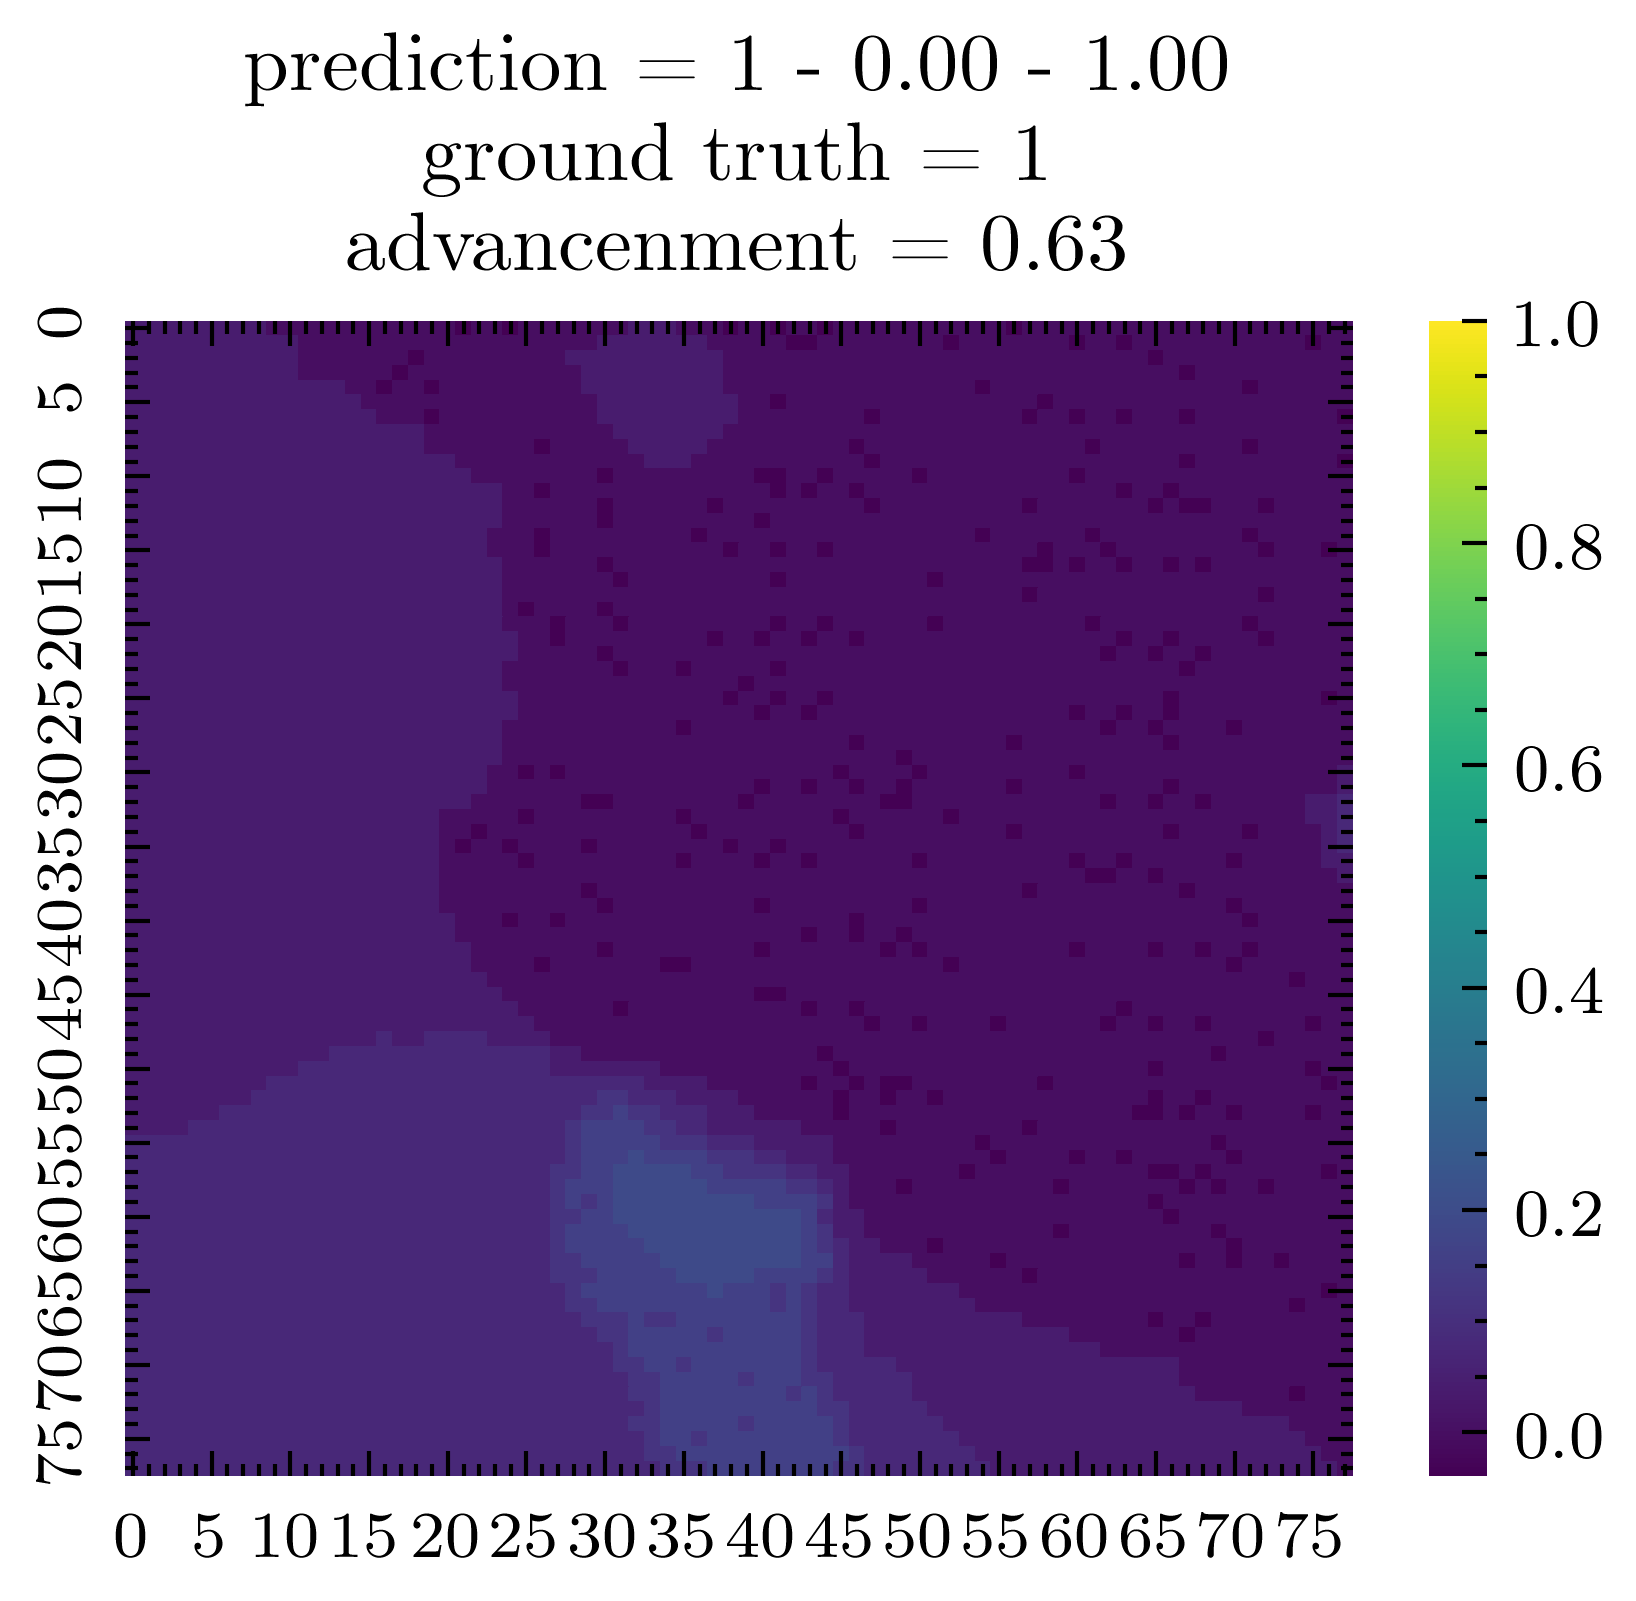
\includegraphics[width=\linewidth]{../img/5/quarry/best/patch-2d-0.png}
    \end{subfigure}
    \begin{subfigure}[b]{0.19\textwidth}
        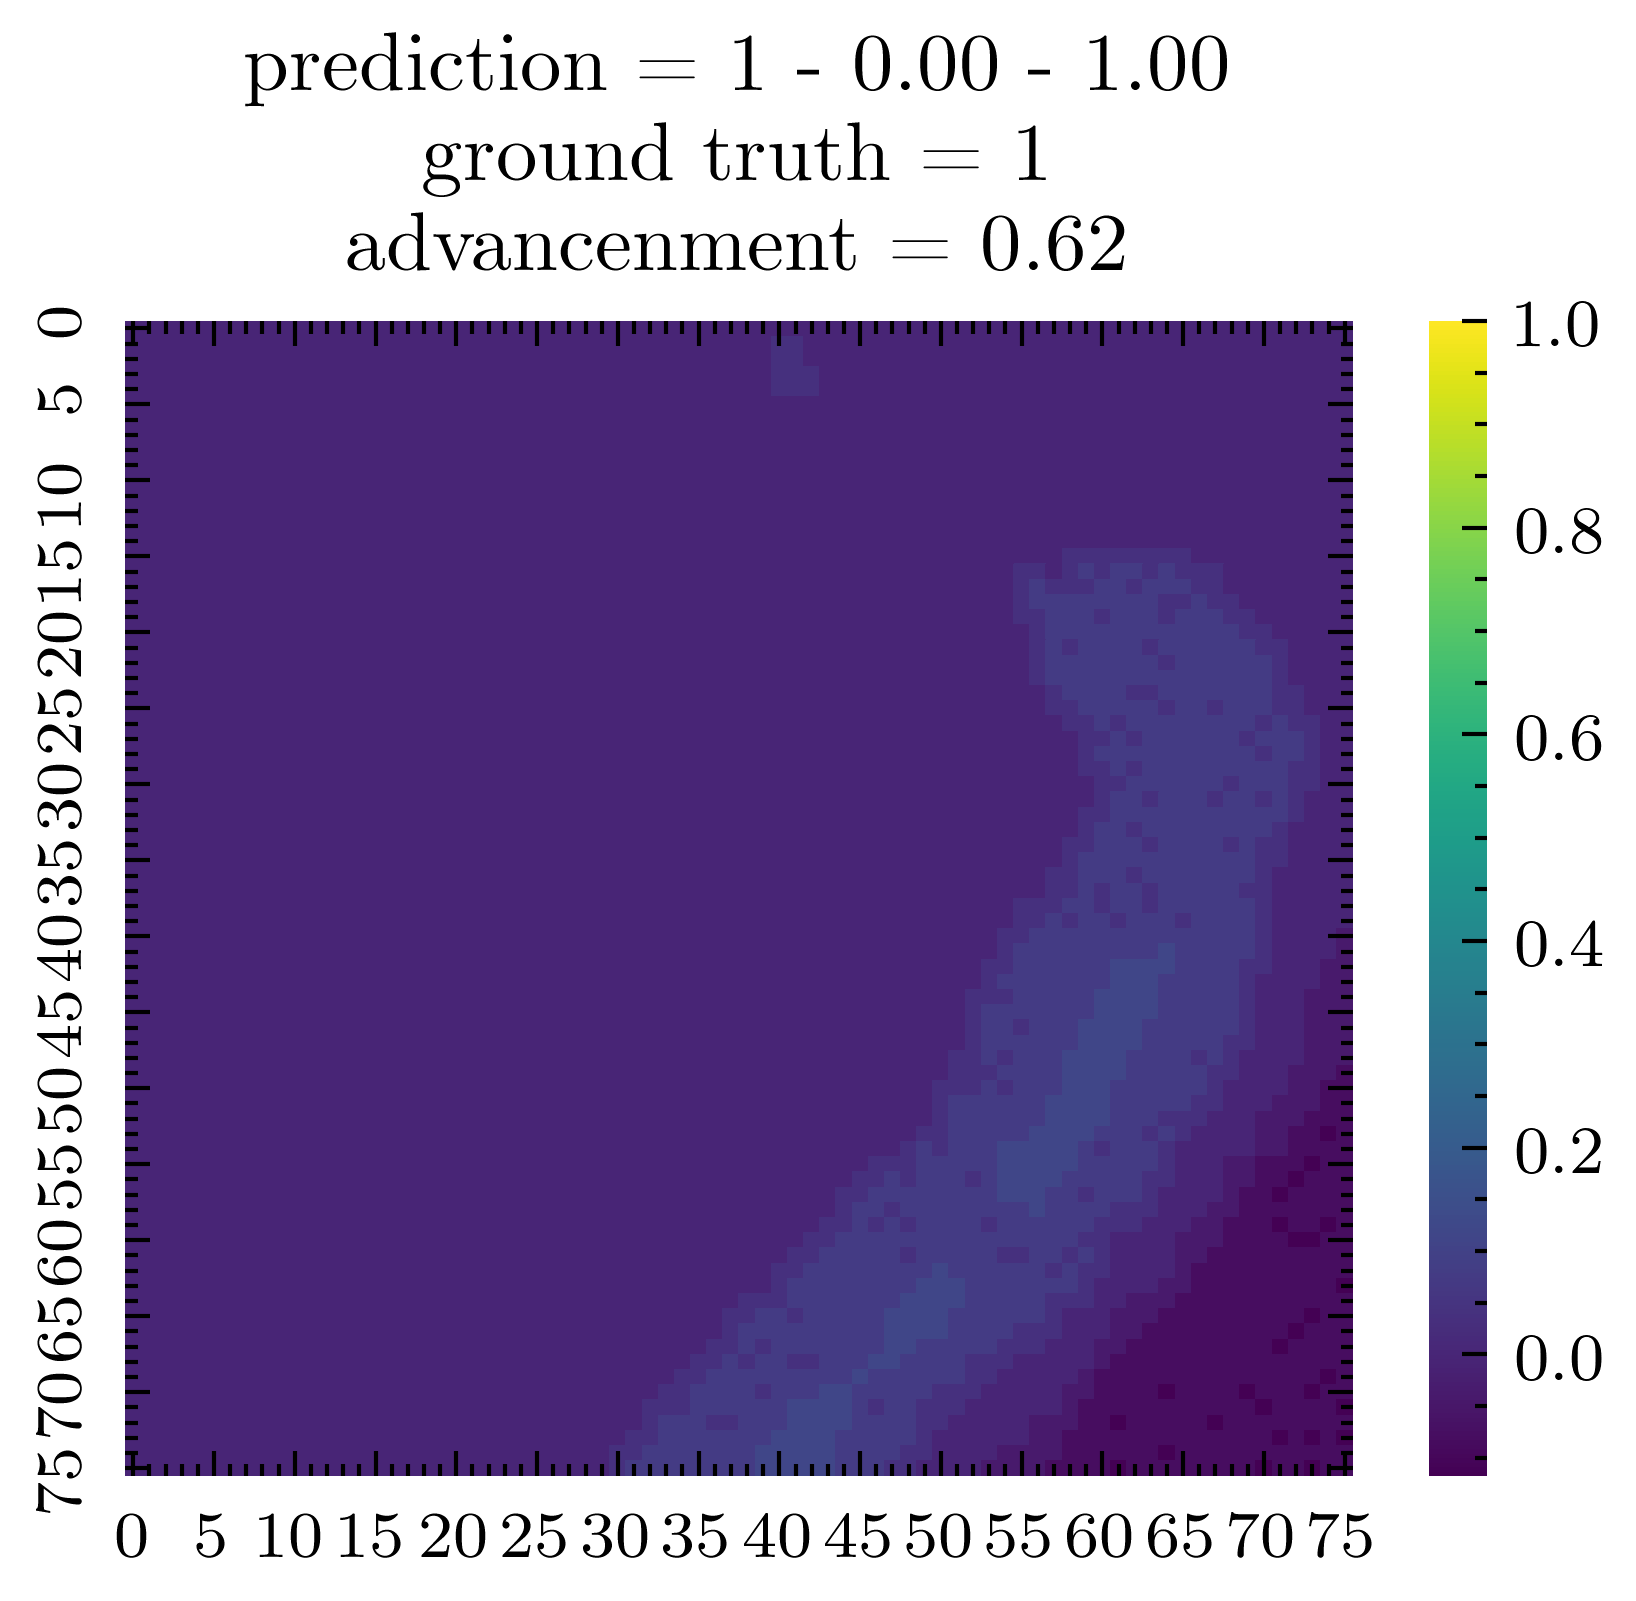
\includegraphics[width=\linewidth]{../img/5/quarry/best/patch-2d-1.png}
    \end{subfigure}  
    \begin{subfigure}[b]{0.19\textwidth}
        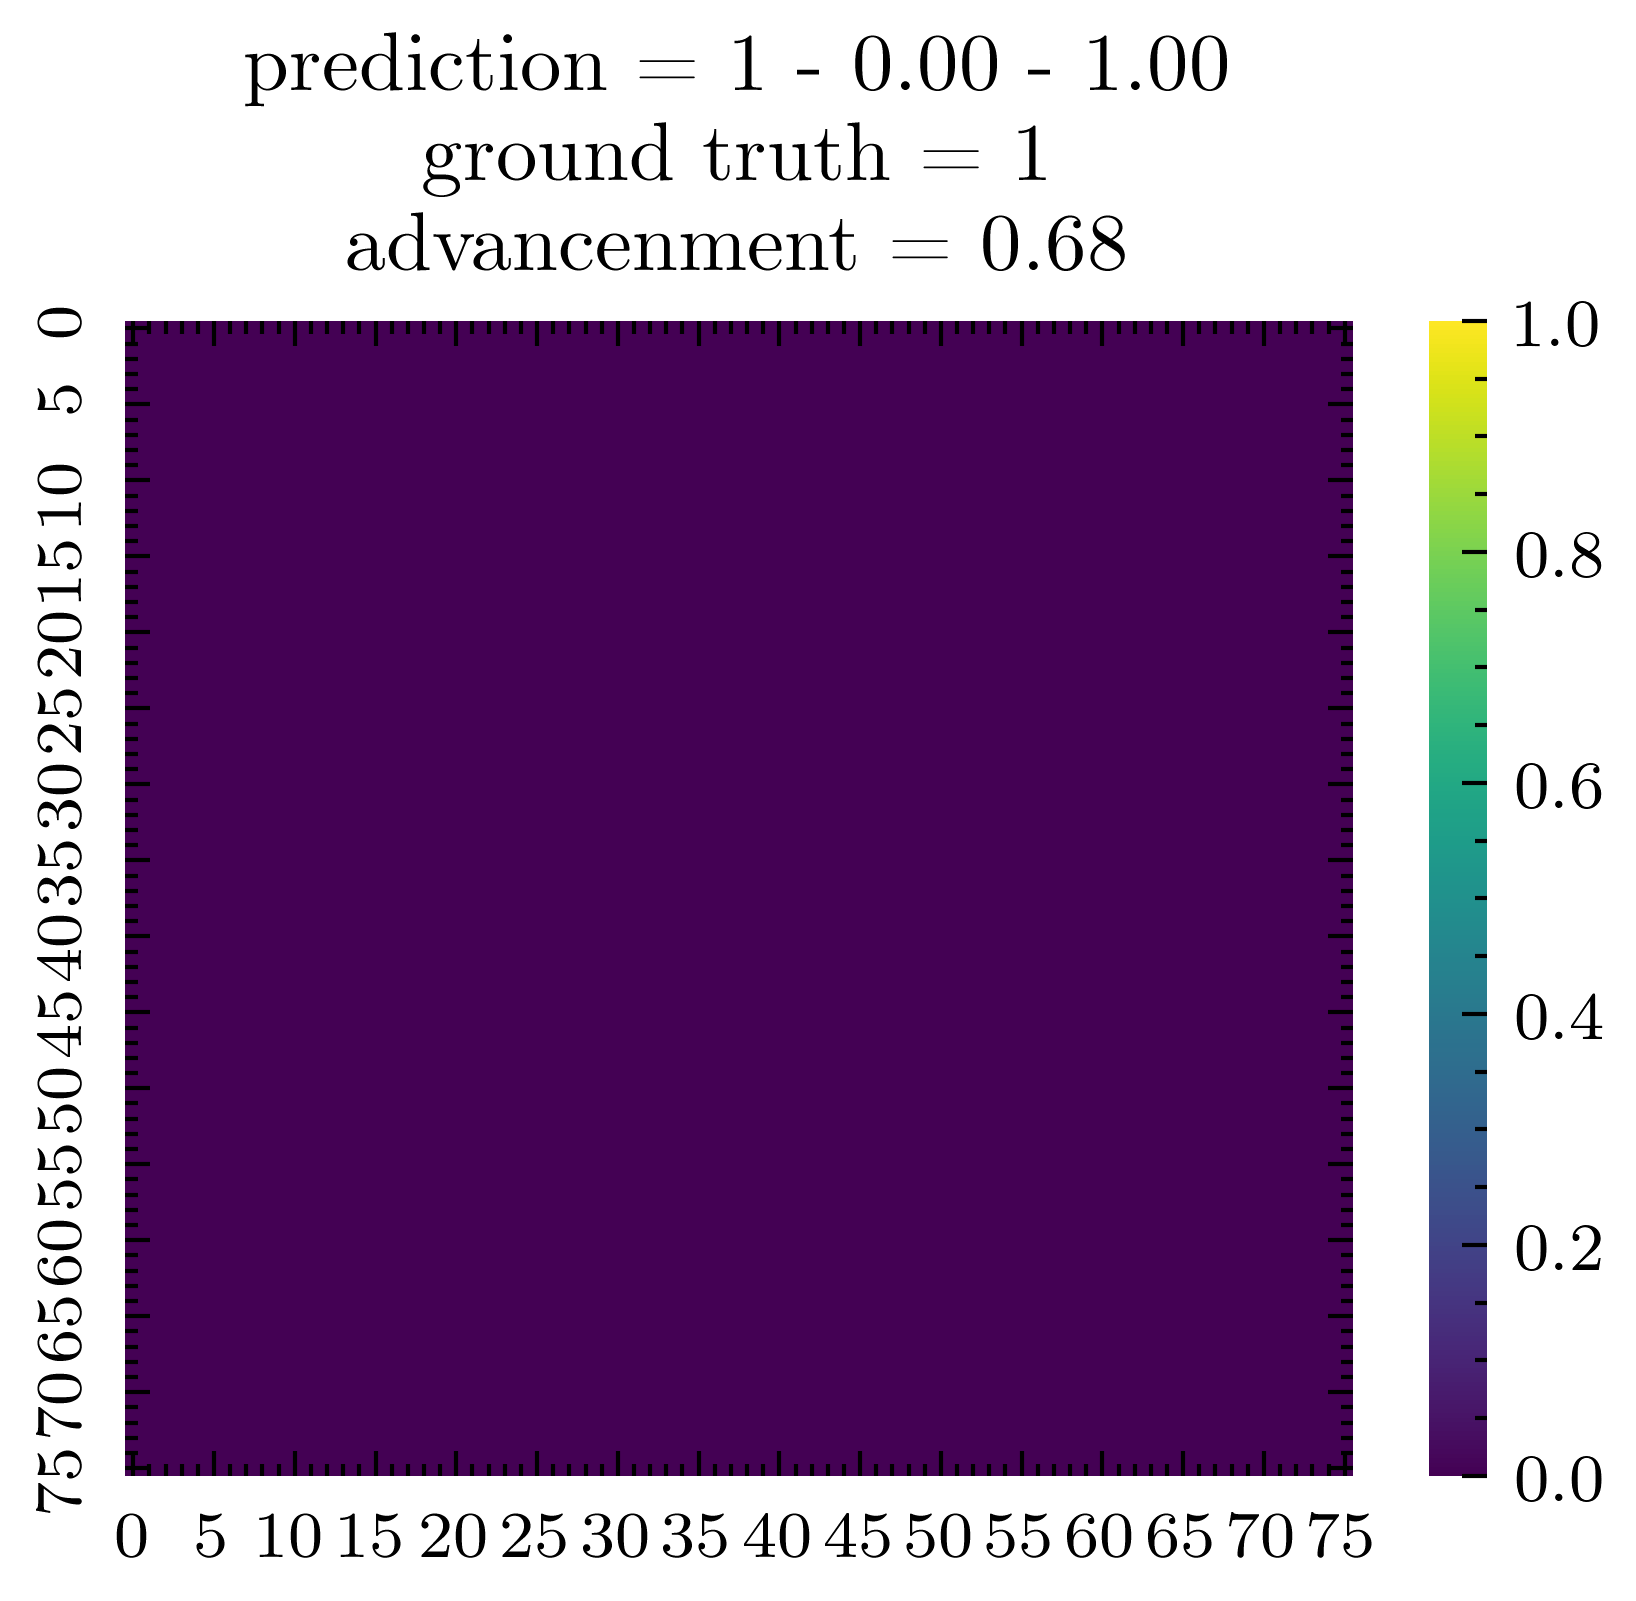
\includegraphics[width=\linewidth]{../img/5/quarry/best/patch-2d-2.png}
    \end{subfigure}
    \begin{subfigure}[b]{0.19\textwidth}
        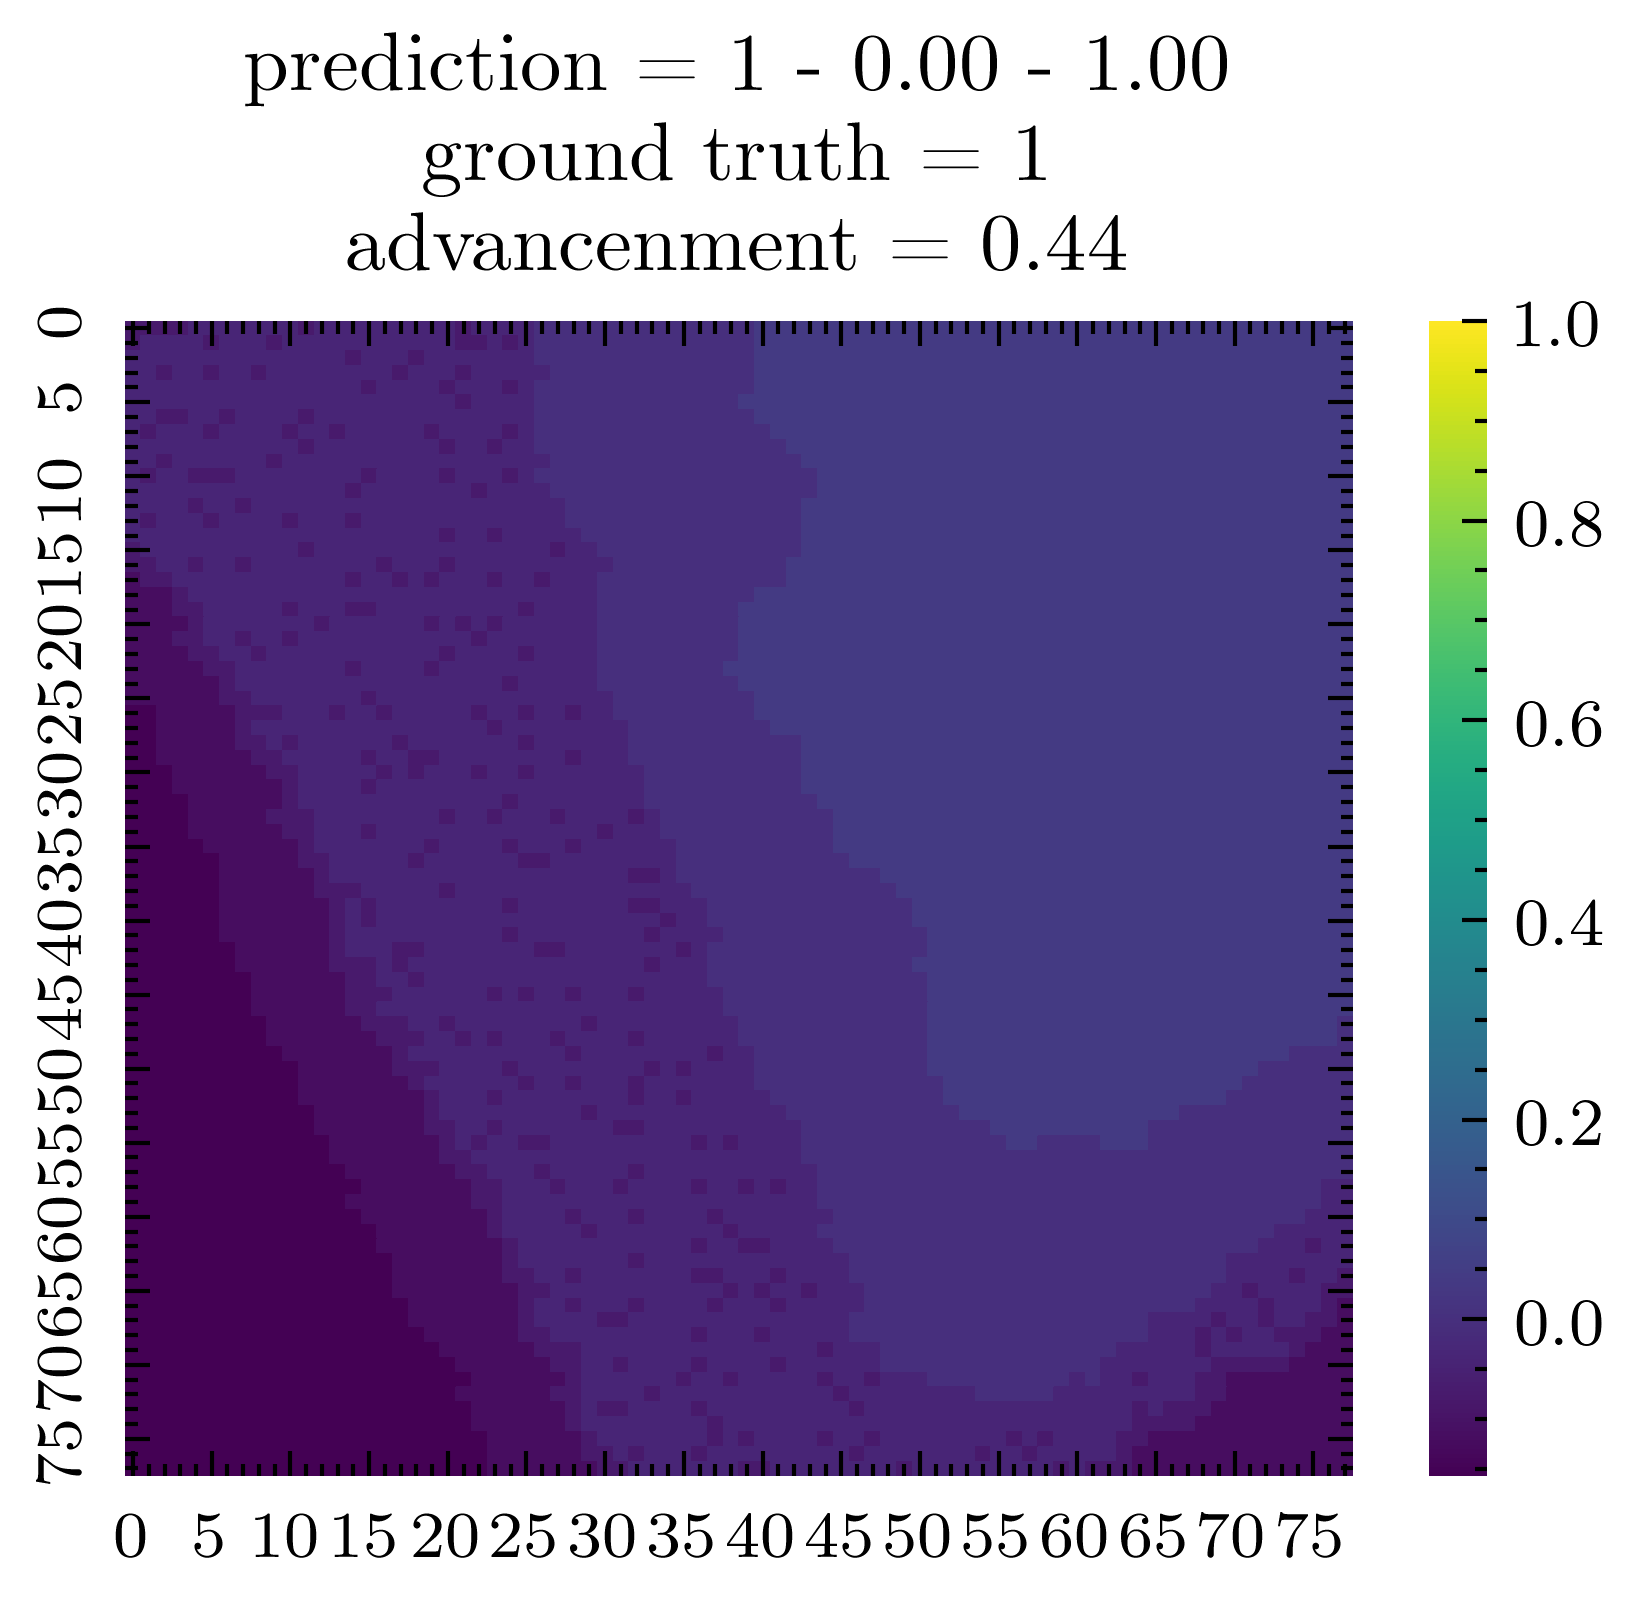
\includegraphics[width=\linewidth]{../img/5/quarry/best/patch-2d-3.png}
    \end{subfigure}  
    \begin{subfigure}[b]{0.19\textwidth}
        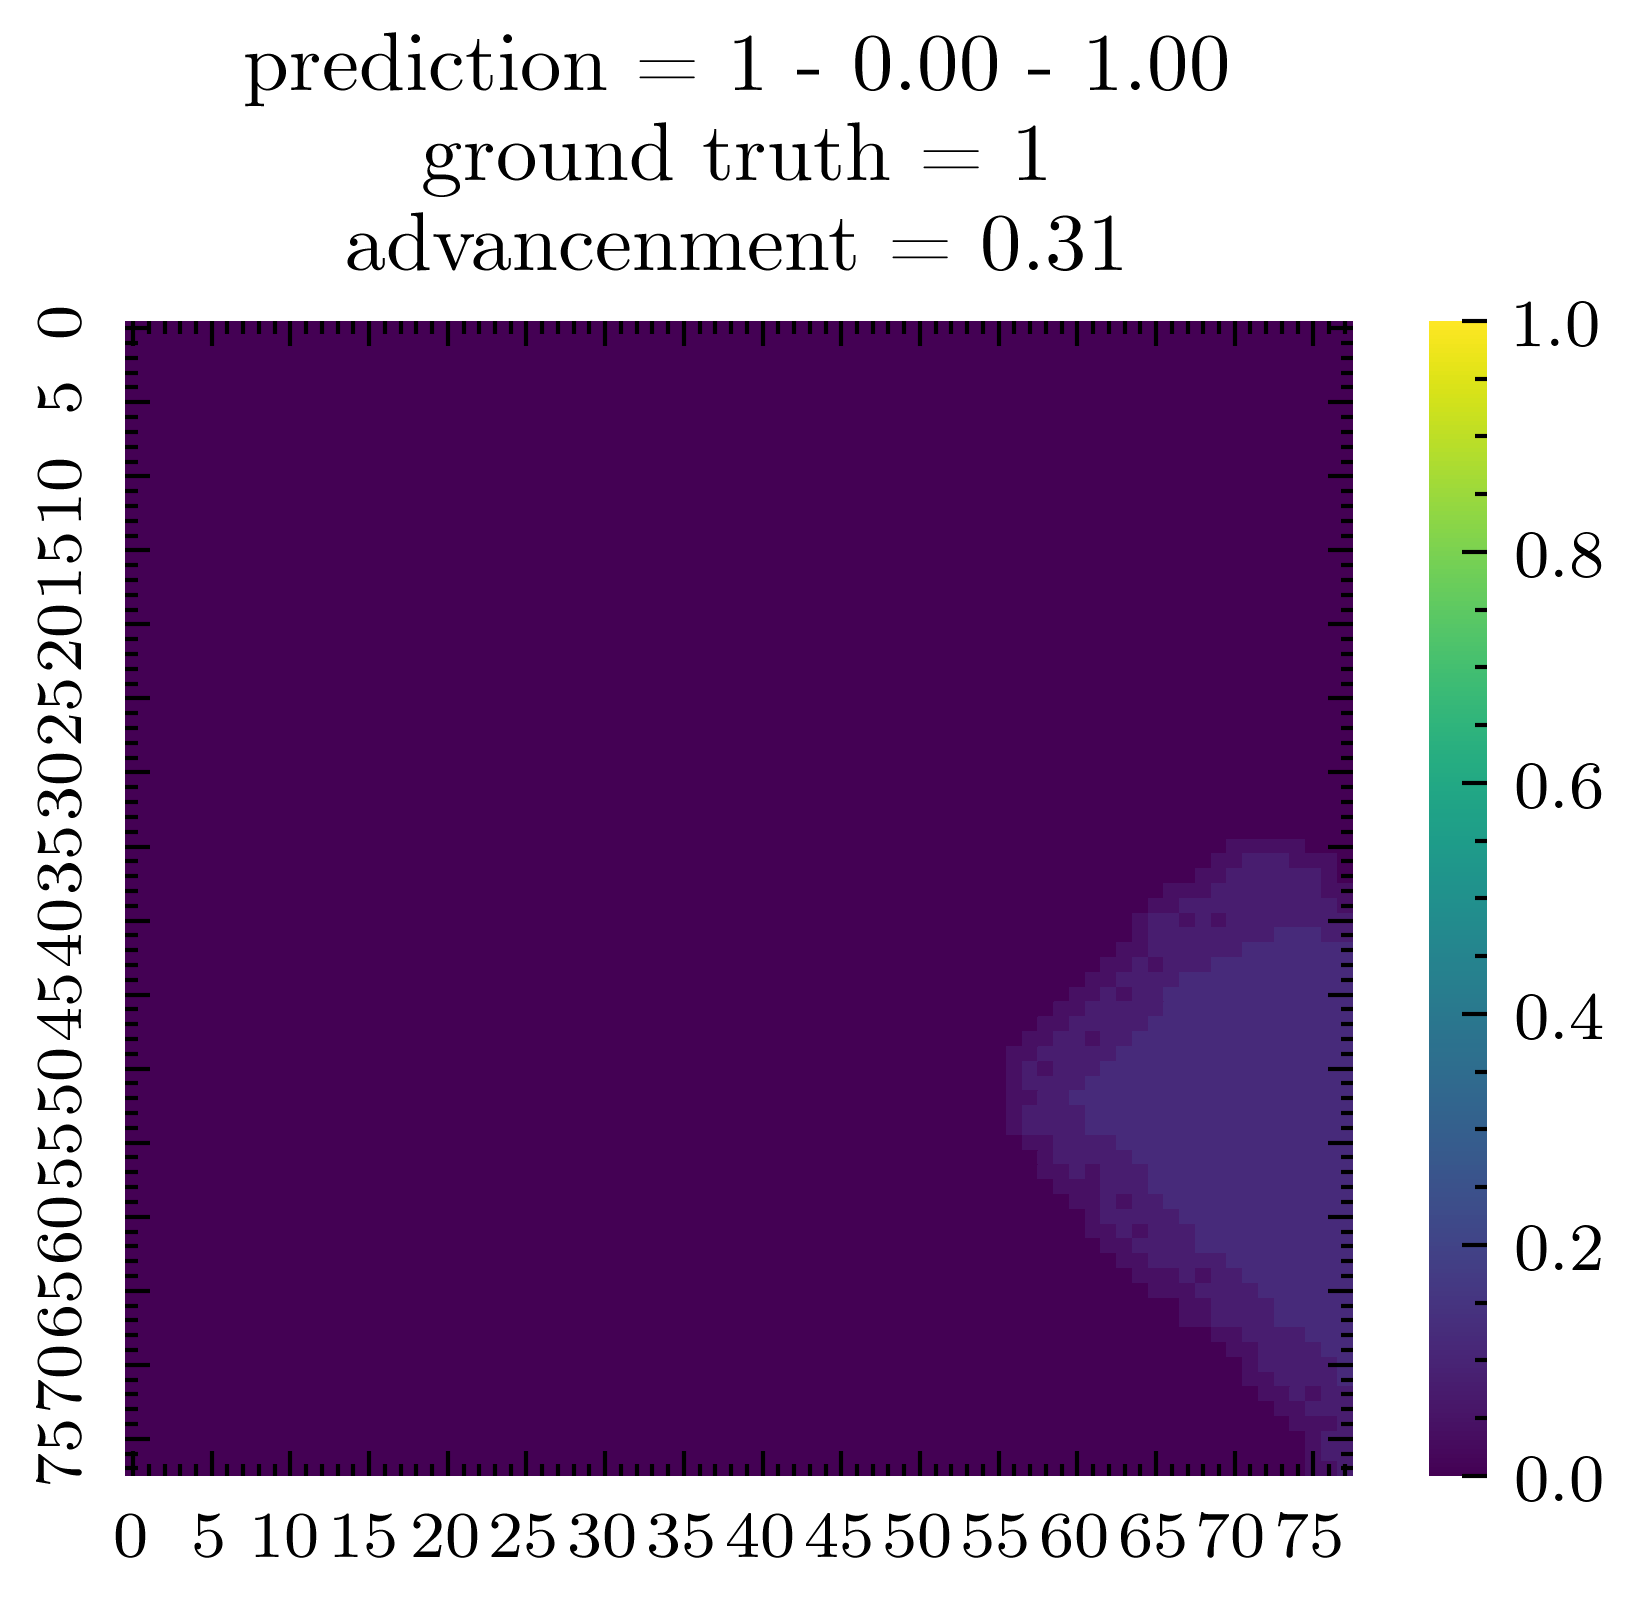
\includegraphics[width=\linewidth]{../img/5/quarry/best/patch-2d-4.png}
    \end{subfigure}  

    \begin{subfigure}[b]{0.19\textwidth}
        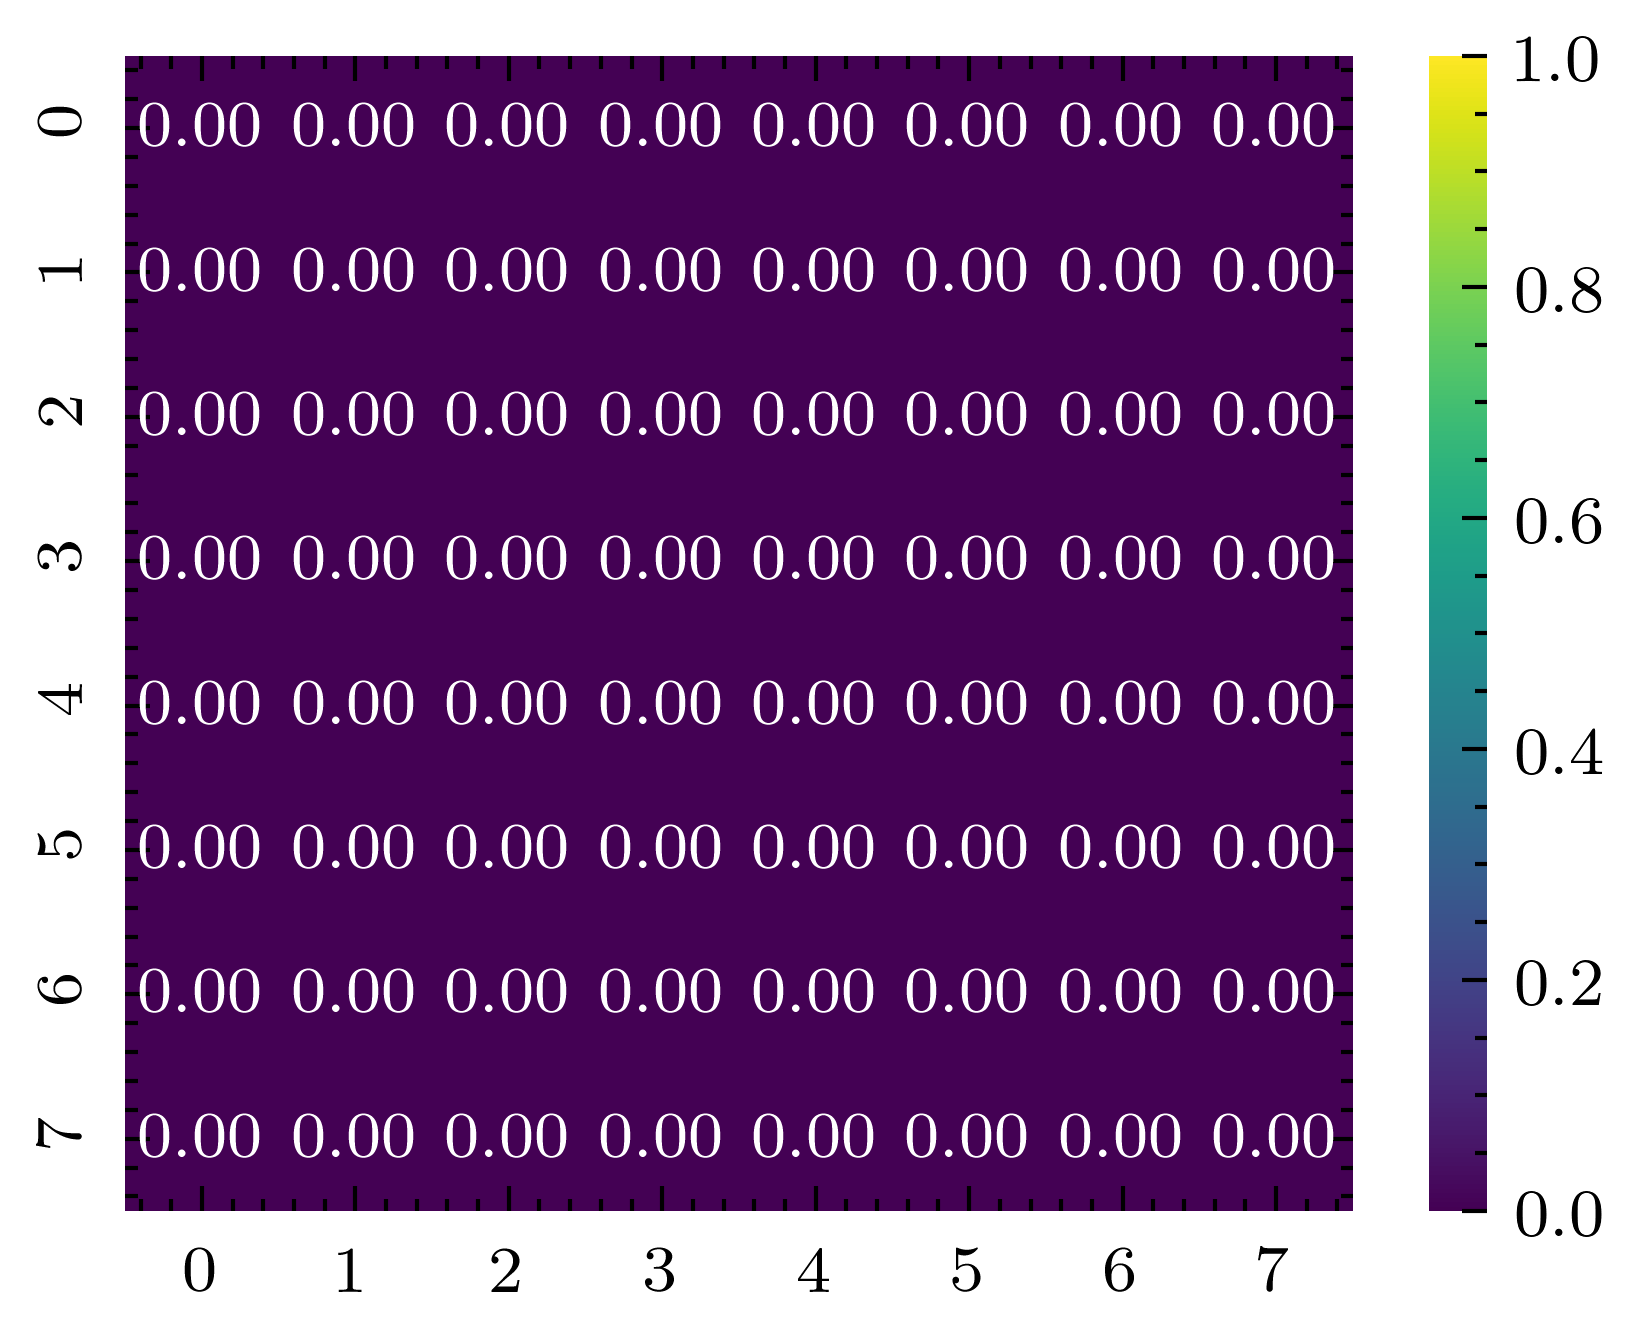
\includegraphics[width=\linewidth]{../img/5/quarry/best/heatmap-2d-0.png}
    \end{subfigure}
    \begin{subfigure}[b]{0.19\textwidth}
        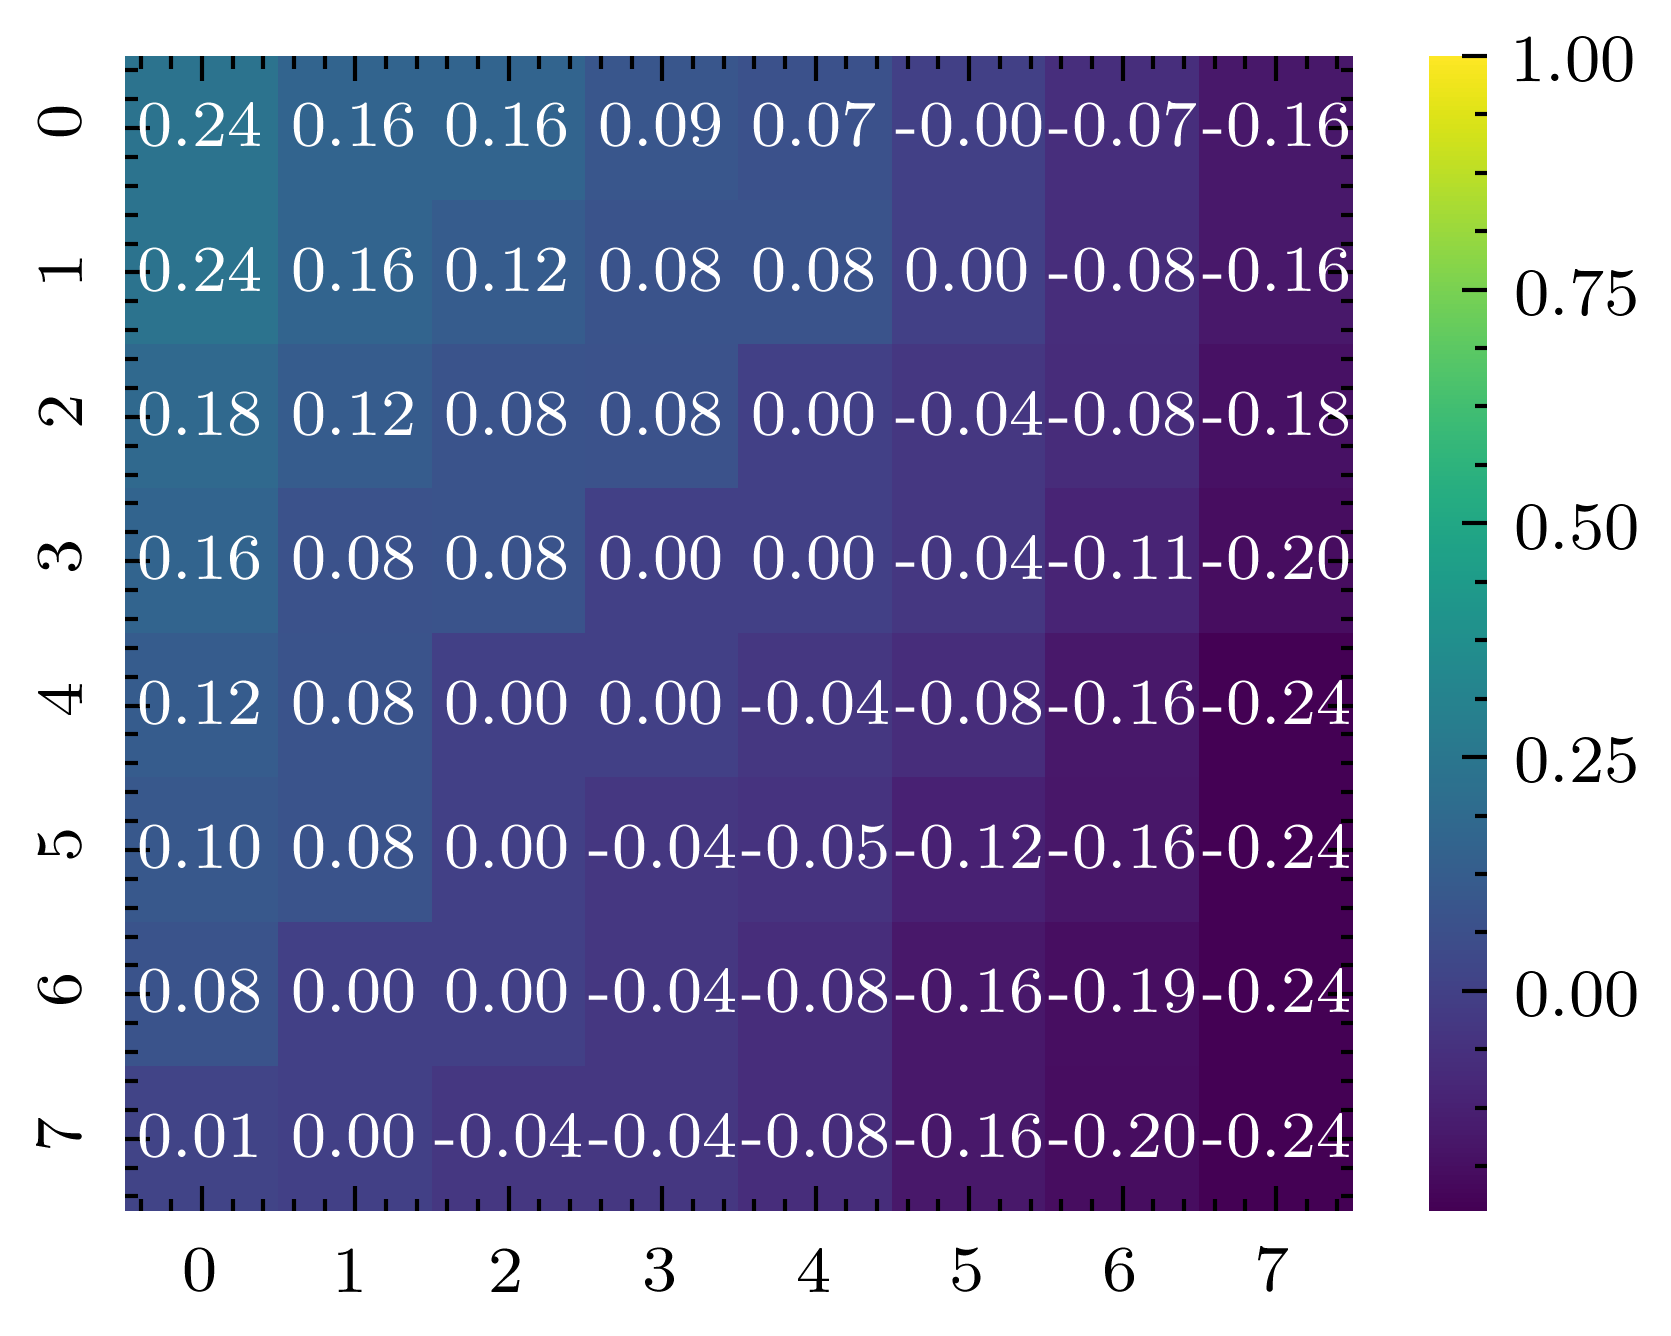
\includegraphics[width=\linewidth]{../img/5/quarry/best/heatmap-2d-1.png}
    \end{subfigure}  
    \begin{subfigure}[b]{0.19\textwidth}
        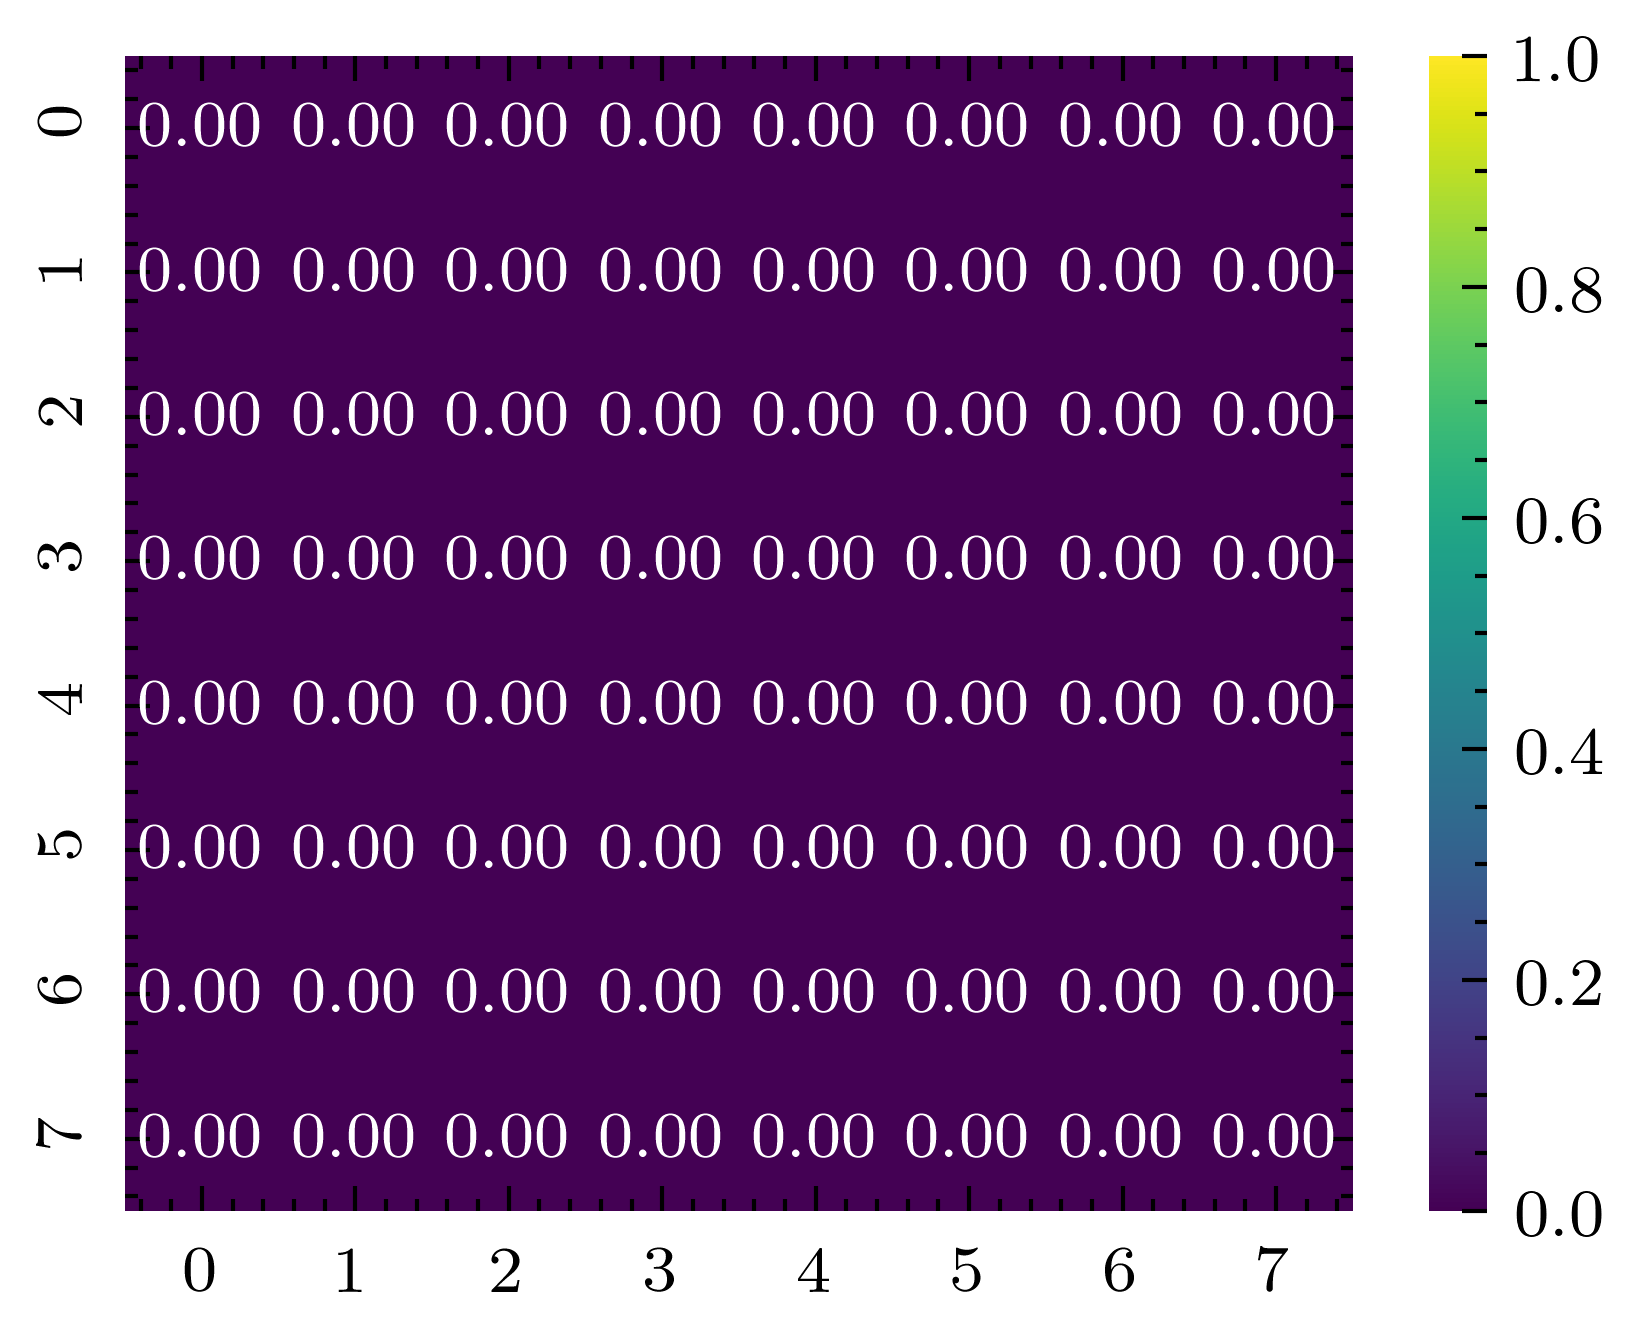
\includegraphics[width=\linewidth]{../img/5/quarry/best/heatmap-2d-2.png}
    \end{subfigure}
    \begin{subfigure}[b]{0.19\textwidth}
        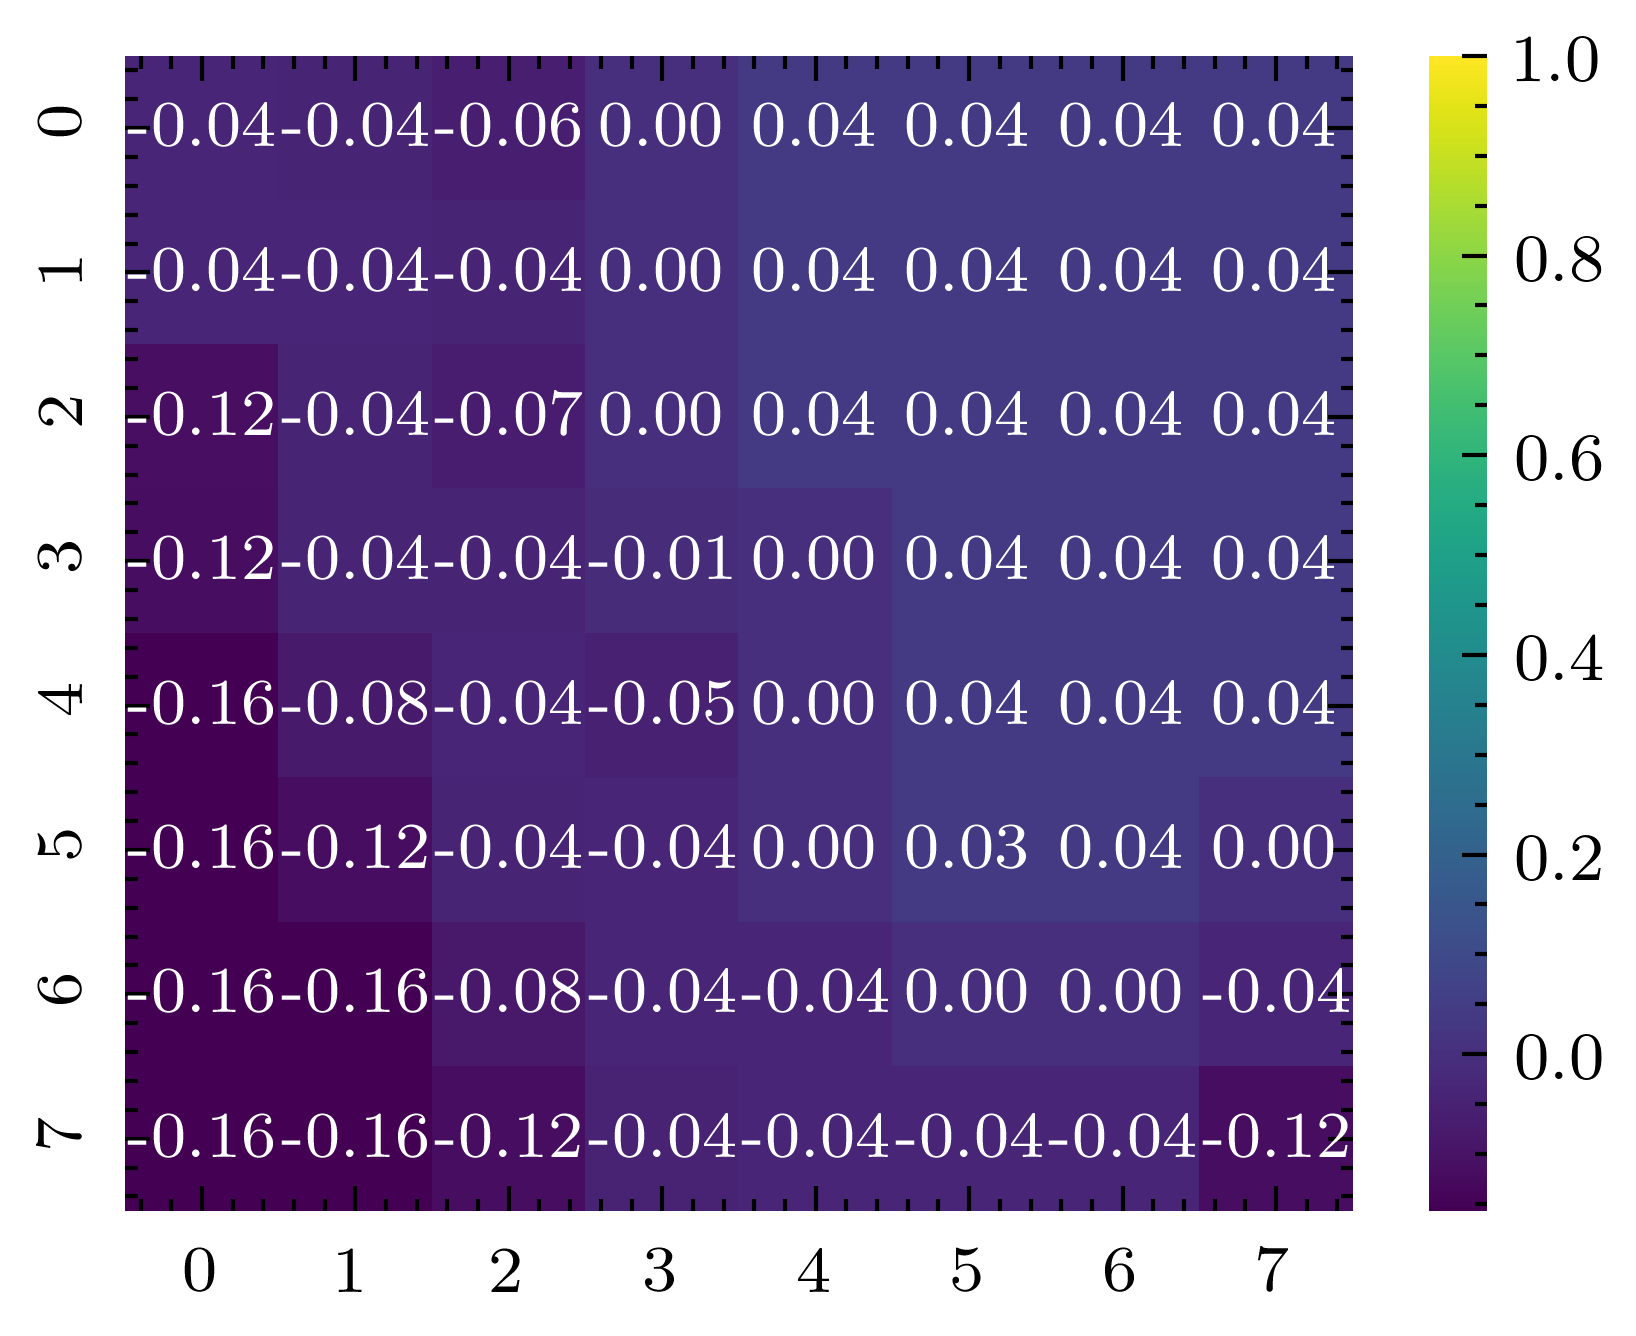
\includegraphics[width=\linewidth]{../img/5/quarry/best/heatmap-2d-3.png}
    \end{subfigure}  
    \begin{subfigure}[b]{0.19\textwidth}
        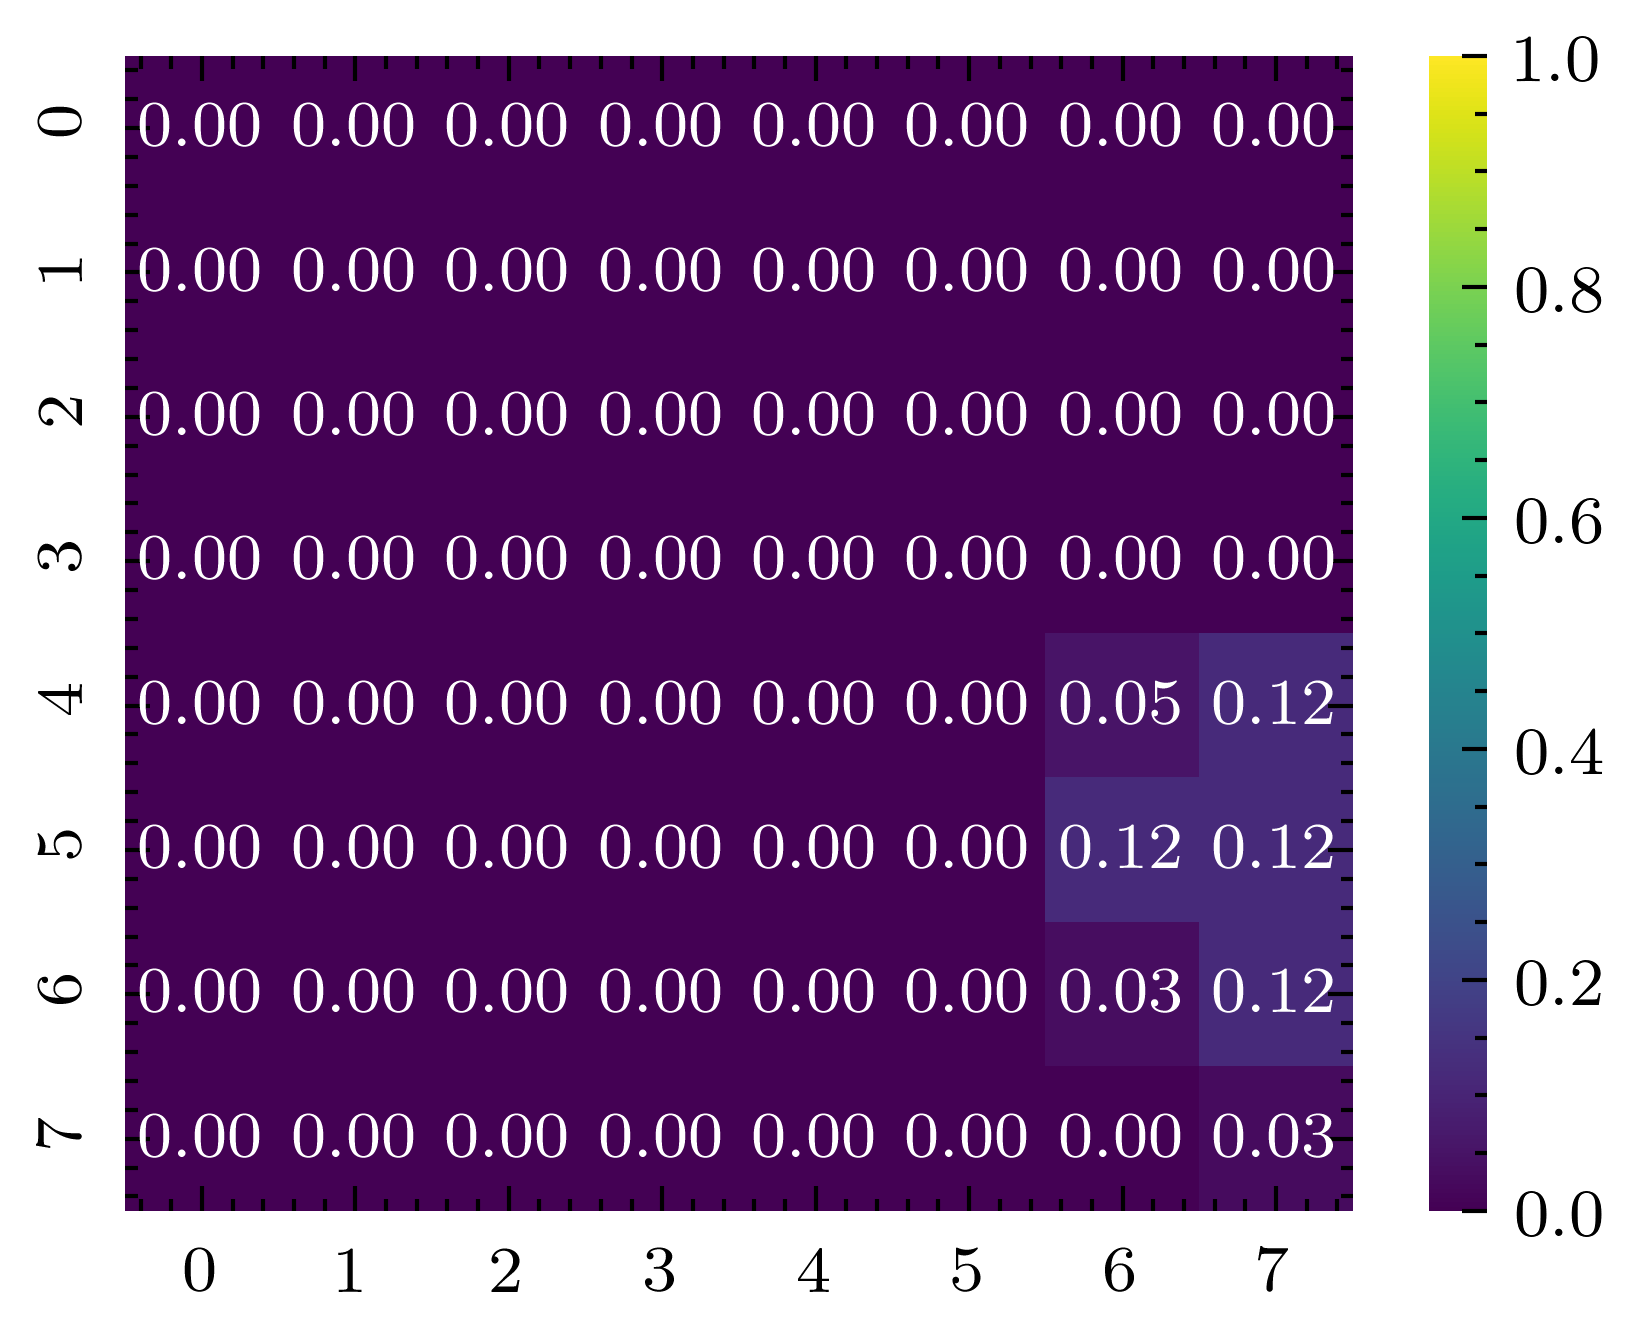
\includegraphics[width=\linewidth]{../img/5/quarry/best/heatmap-2d-4.png}
    \end{subfigure}  

    \begin{subfigure}[b]{0.19\textwidth}
        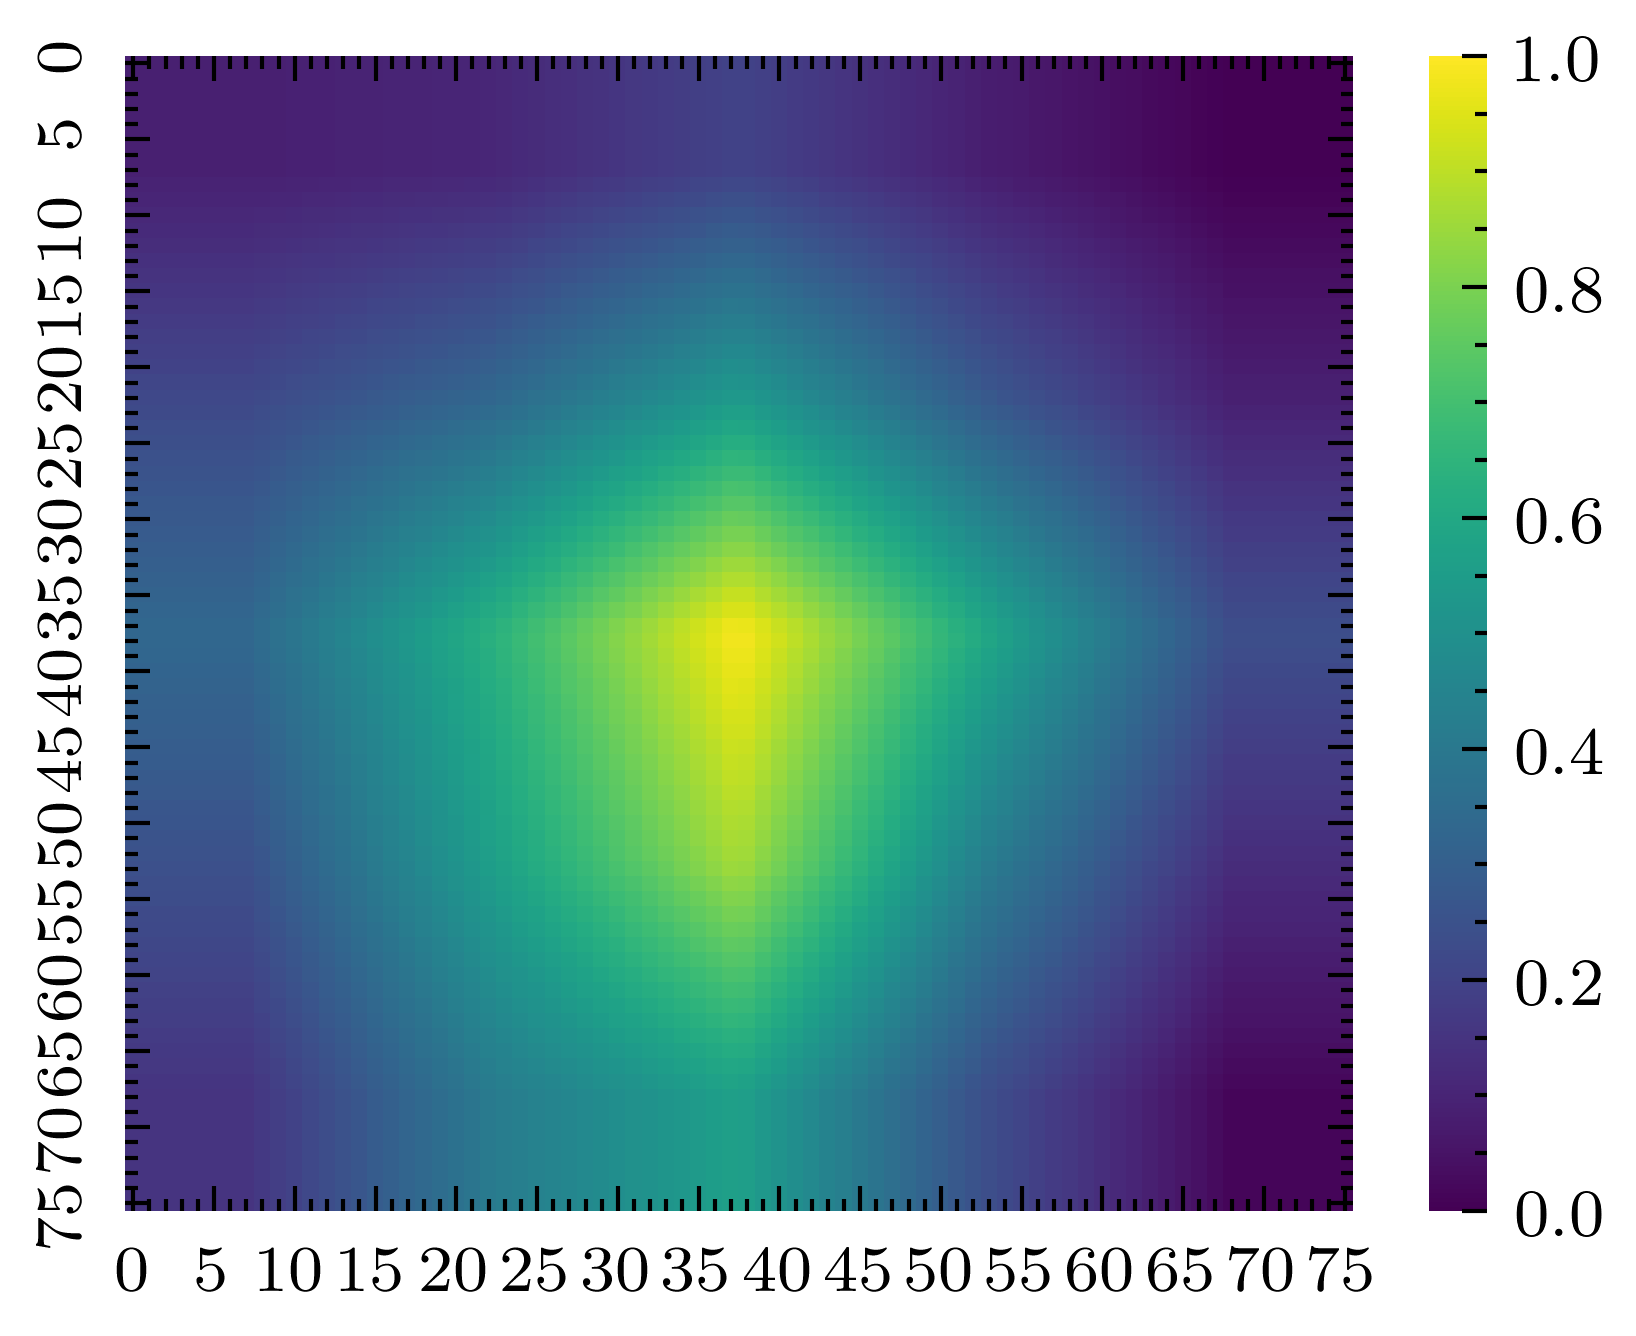
\includegraphics[width=\linewidth]{../img/5/quarry/best/grad-cam-2d-0.png}
    \end{subfigure}
    \begin{subfigure}[b]{0.19\textwidth}
        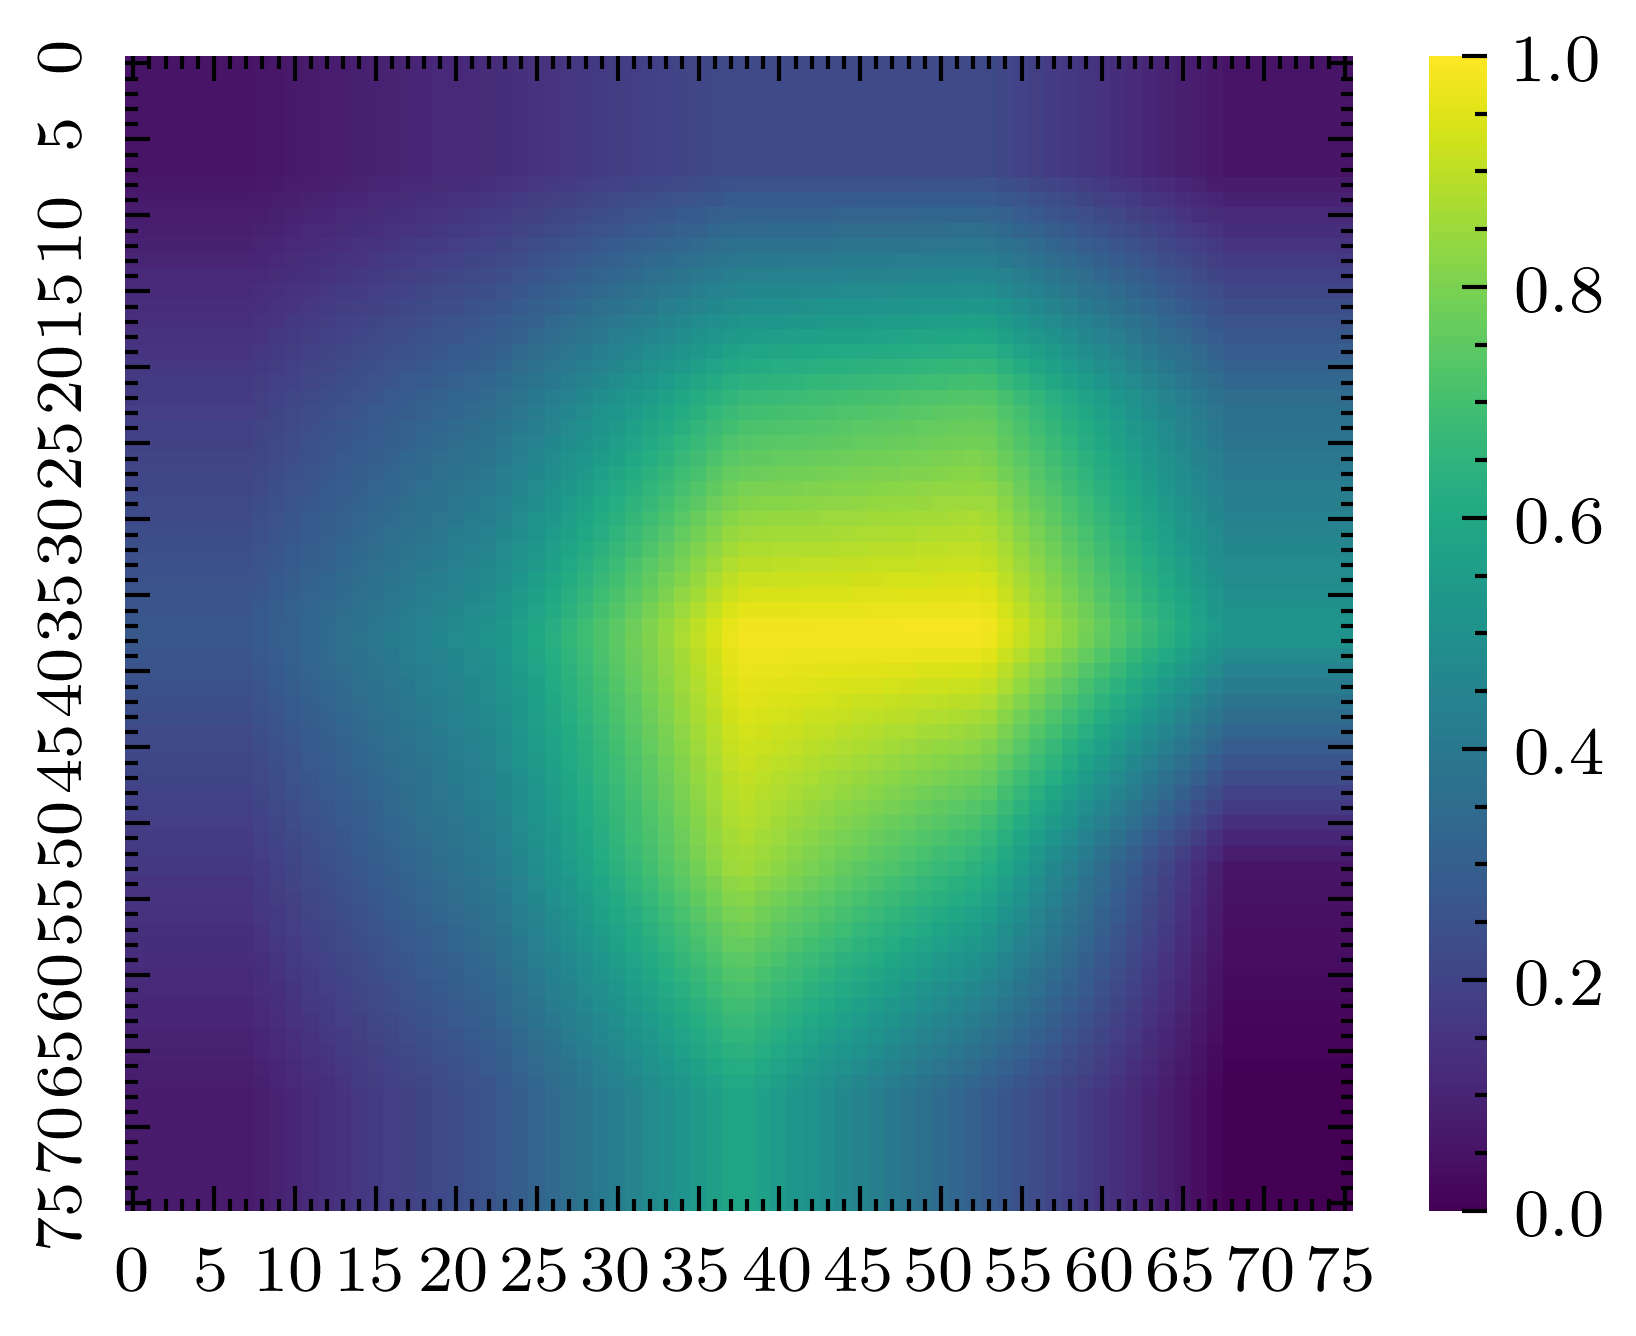
\includegraphics[width=\linewidth]{../img/5/quarry/best/grad-cam-2d-1.png}
    \end{subfigure}  
    \begin{subfigure}[b]{0.19\textwidth}
        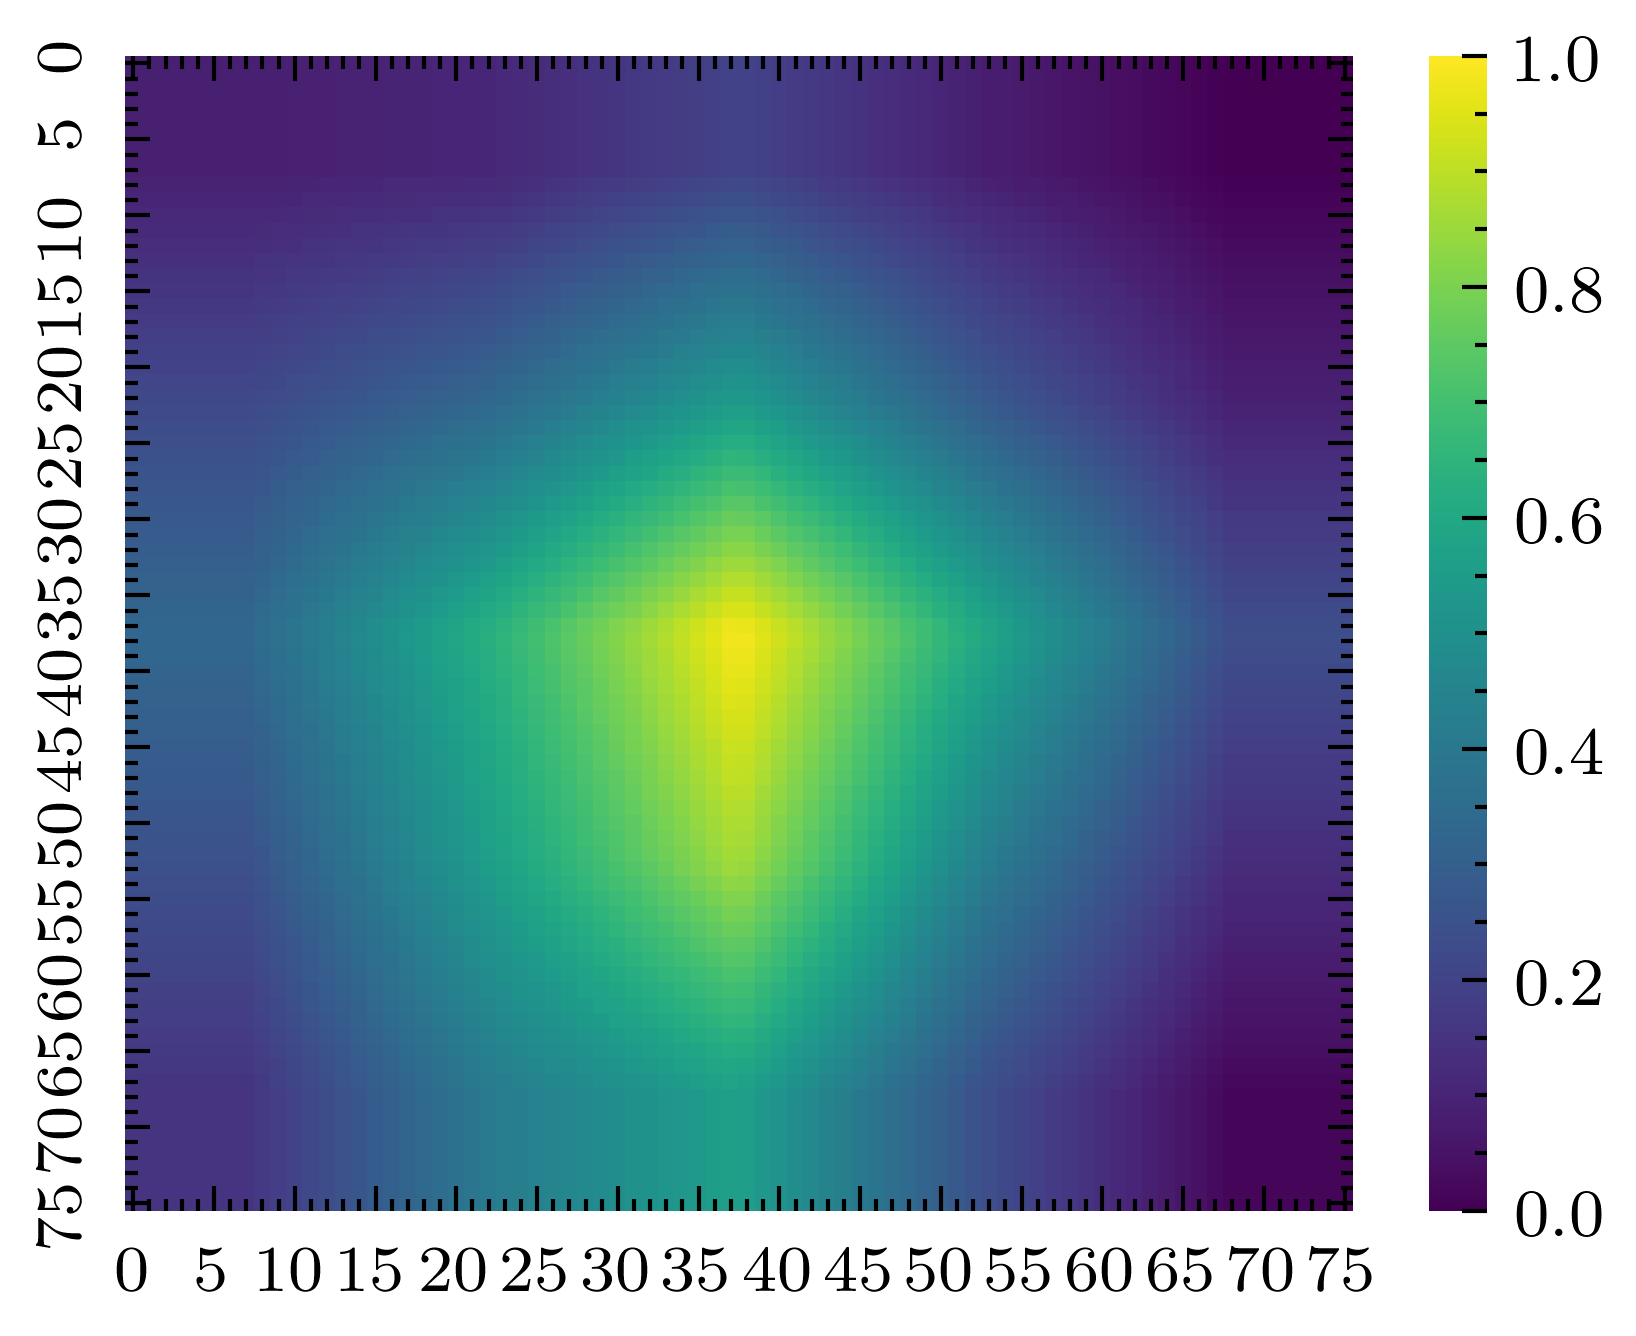
\includegraphics[width=\linewidth]{../img/5/quarry/best/grad-cam-2d-2.png}
    \end{subfigure}
    \begin{subfigure}[b]{0.19\textwidth}
        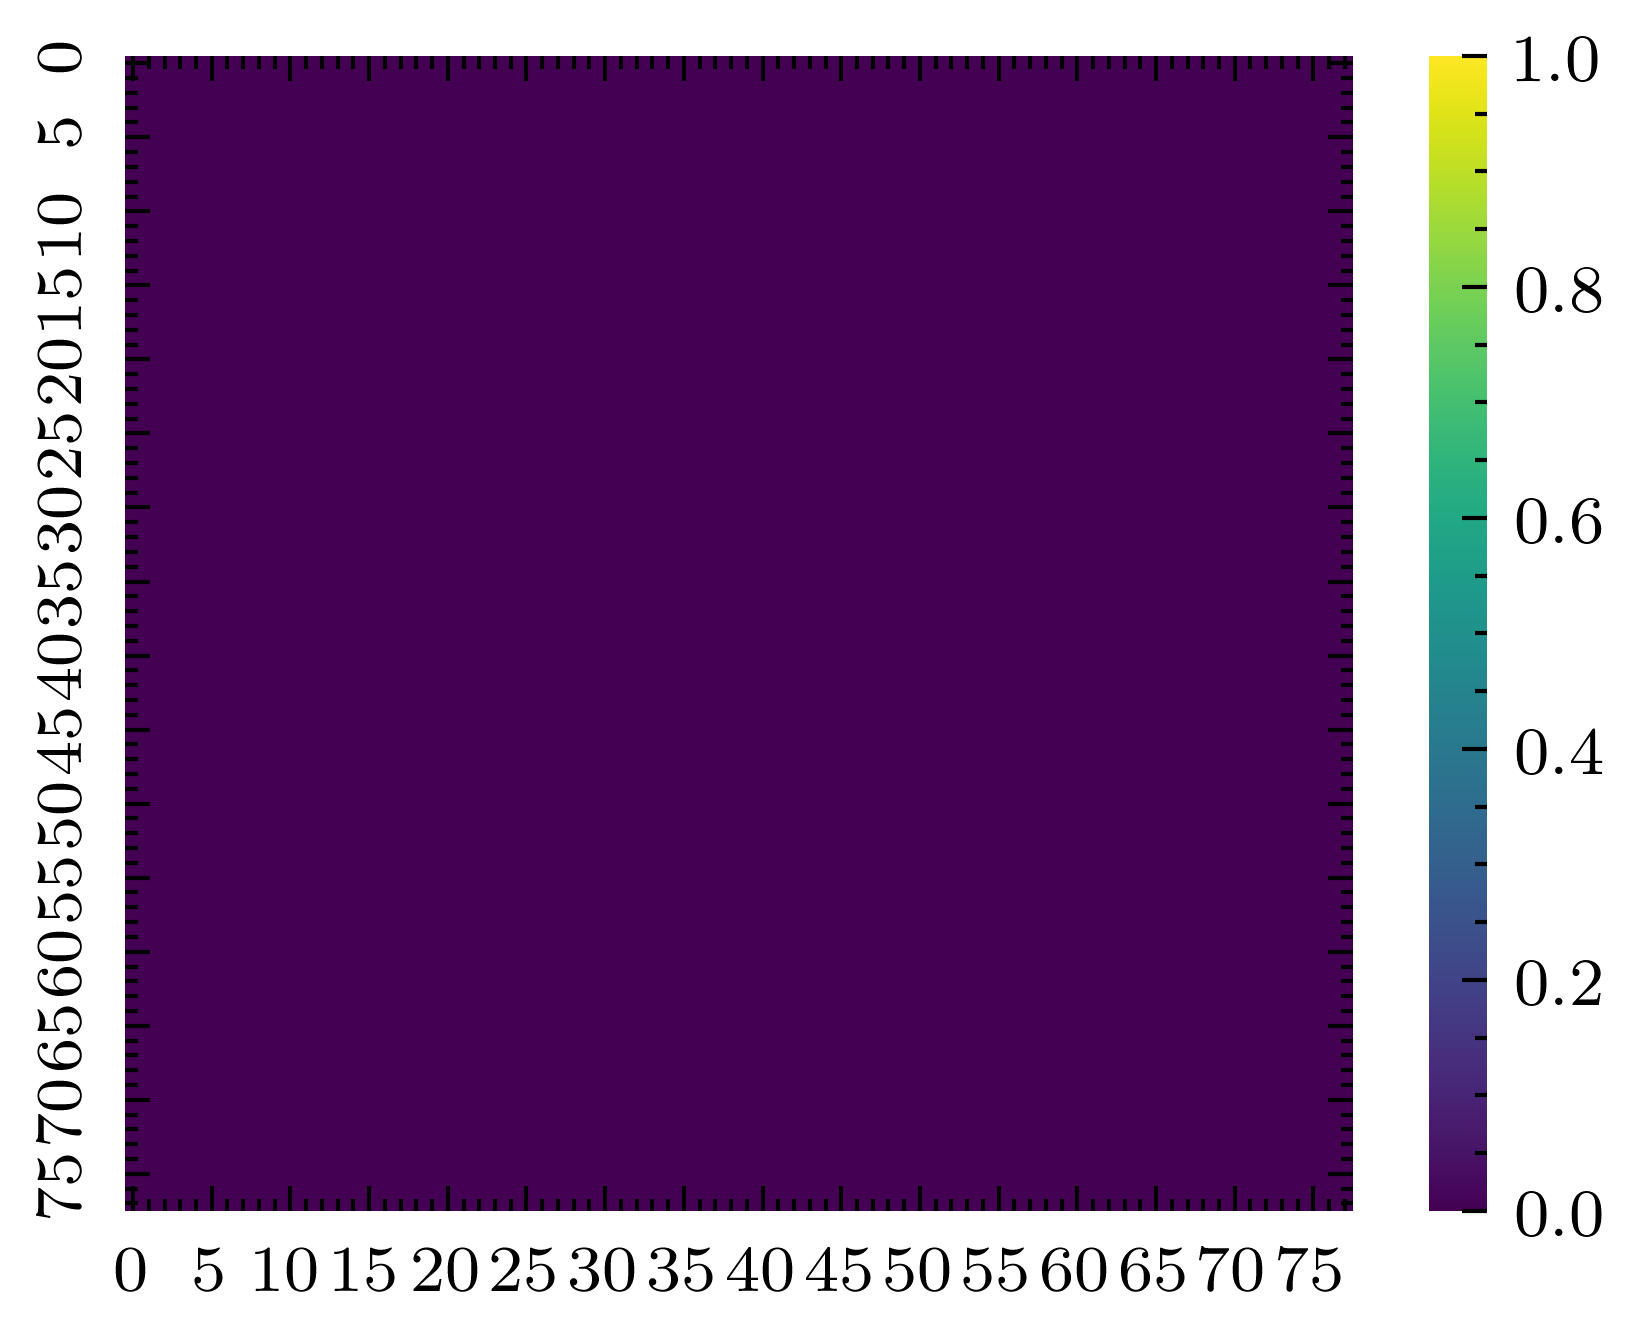
\includegraphics[width=\linewidth]{../img/5/quarry/best/grad-cam-2d-3.png}
    \end{subfigure}  
    \begin{subfigure}[b]{0.19\textwidth}
        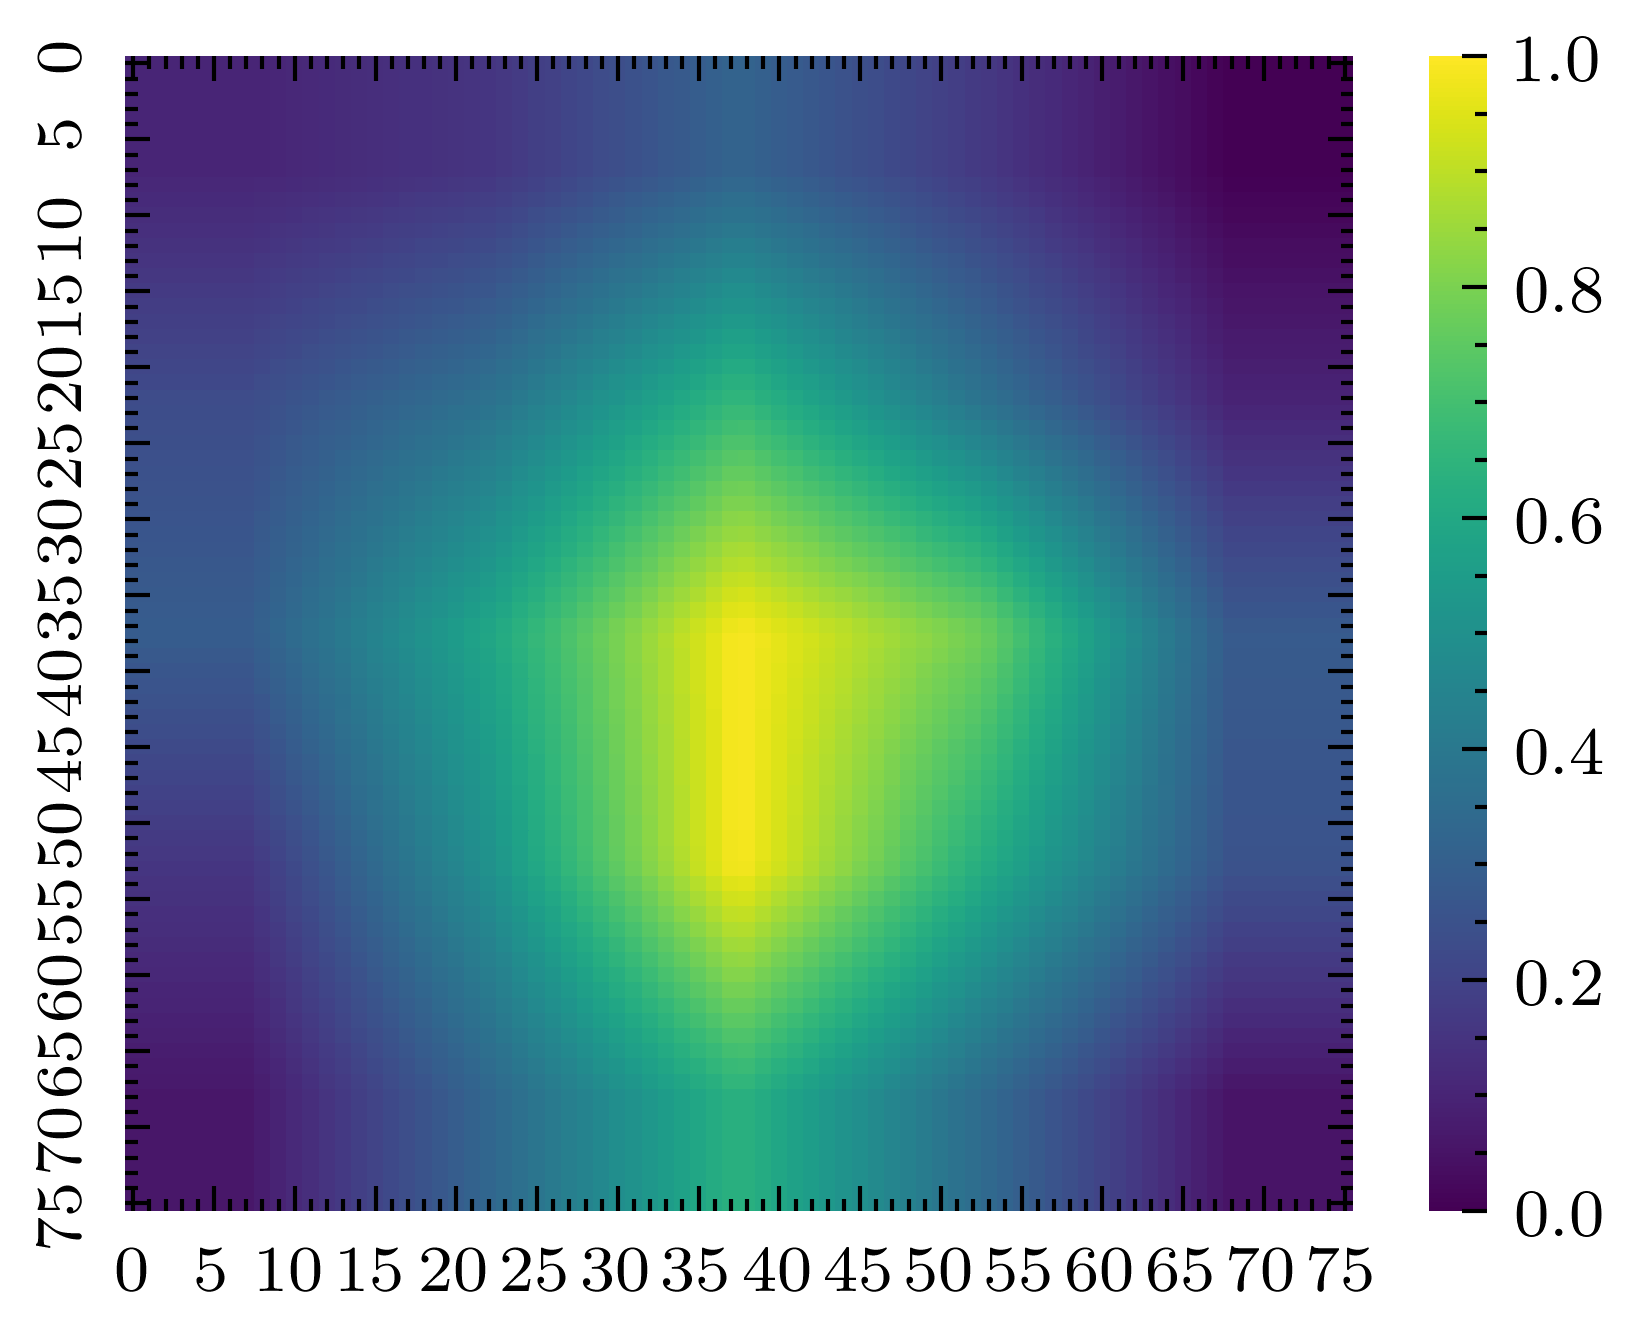
\includegraphics[width=\linewidth]{../img/5/quarry/best/grad-cam-2d-4.png}
    \end{subfigure}  

    \begin{subfigure}[b]{0.19\textwidth}
        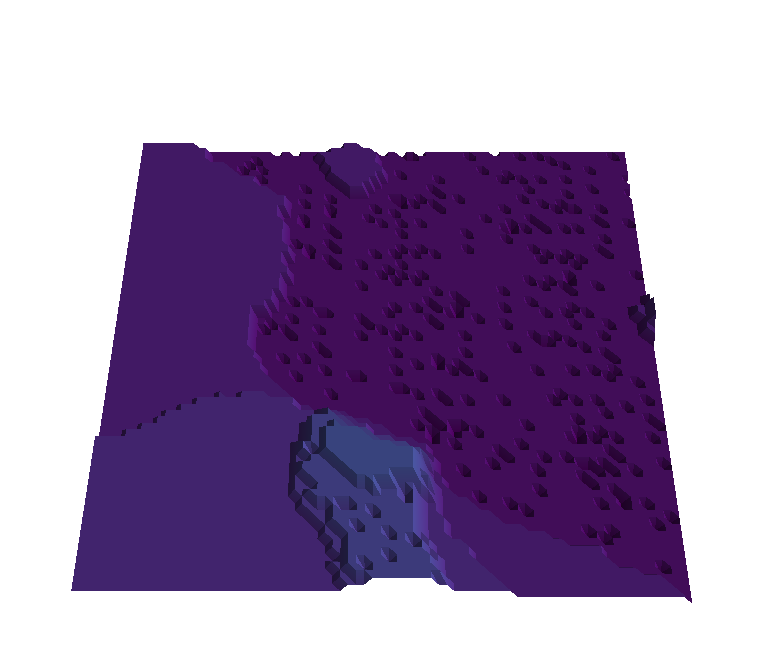
\includegraphics[width=\linewidth]{../img/5/quarry/best//patch-3d-majavi-colormap-0.png}
    \end{subfigure}
    \begin{subfigure}[b]{0.19\textwidth}
        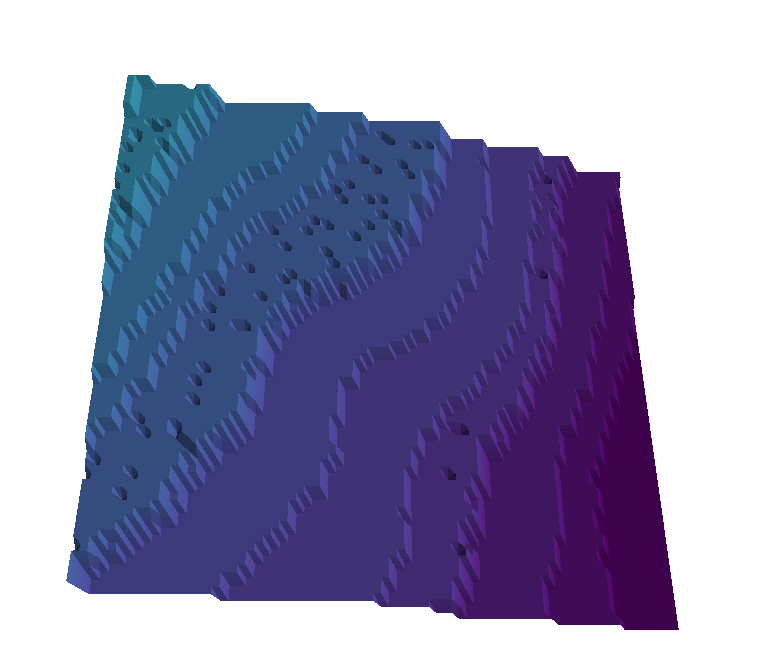
\includegraphics[width=\linewidth]{../img/5/quarry/best//patch-3d-majavi-colormap-1.png}
    \end{subfigure}  
    \begin{subfigure}[b]{0.19\textwidth}
        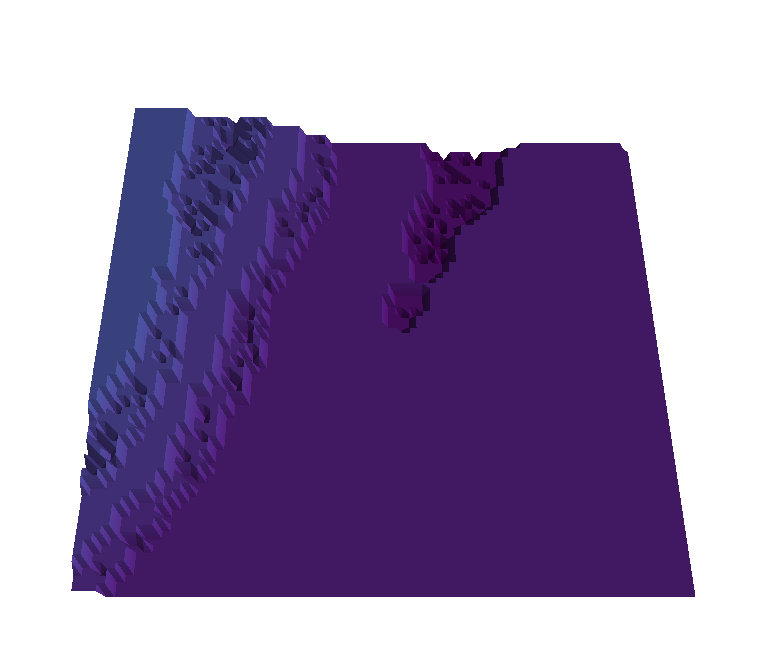
\includegraphics[width=\linewidth]{../img/5/quarry/best//patch-3d-majavi-colormap-2.png}
    \end{subfigure}
    \begin{subfigure}[b]{0.19\textwidth}
        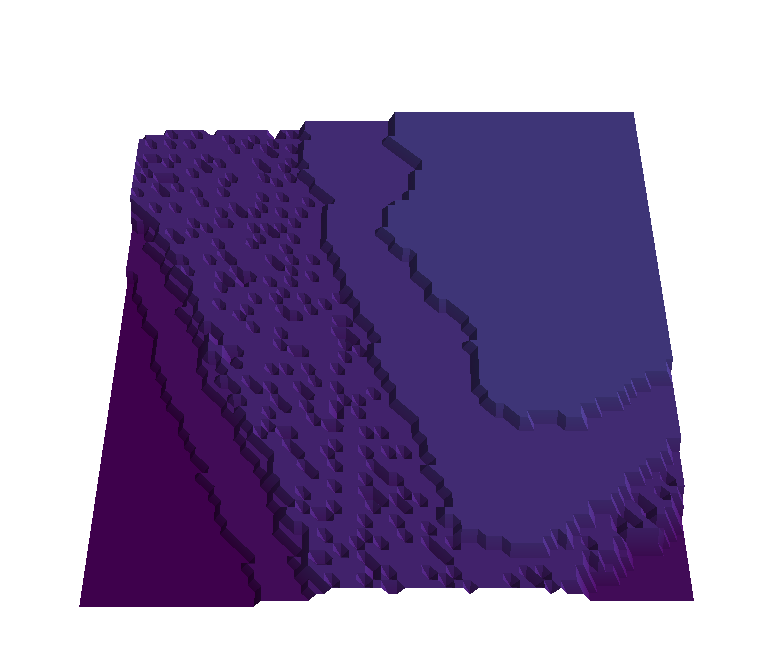
\includegraphics[width=\linewidth]{../img/5/quarry/best//patch-3d-majavi-colormap-3.png}
    \end{subfigure}  
    \begin{subfigure}[b]{0.19\textwidth}
        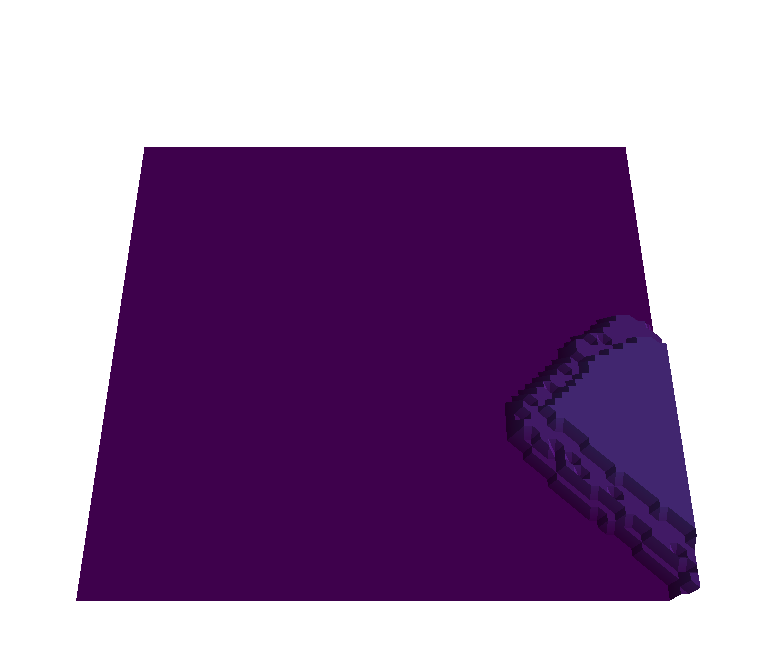
\includegraphics[width=\linewidth]{../img/5/quarry/best//patch-3d-majavi-colormap-4.png}
    \end{subfigure}  

\caption{Best}    
\end{figure}


\begin{figure}[H]
    \centering
    \begin{subfigure}[b]{0.19\textwidth}
        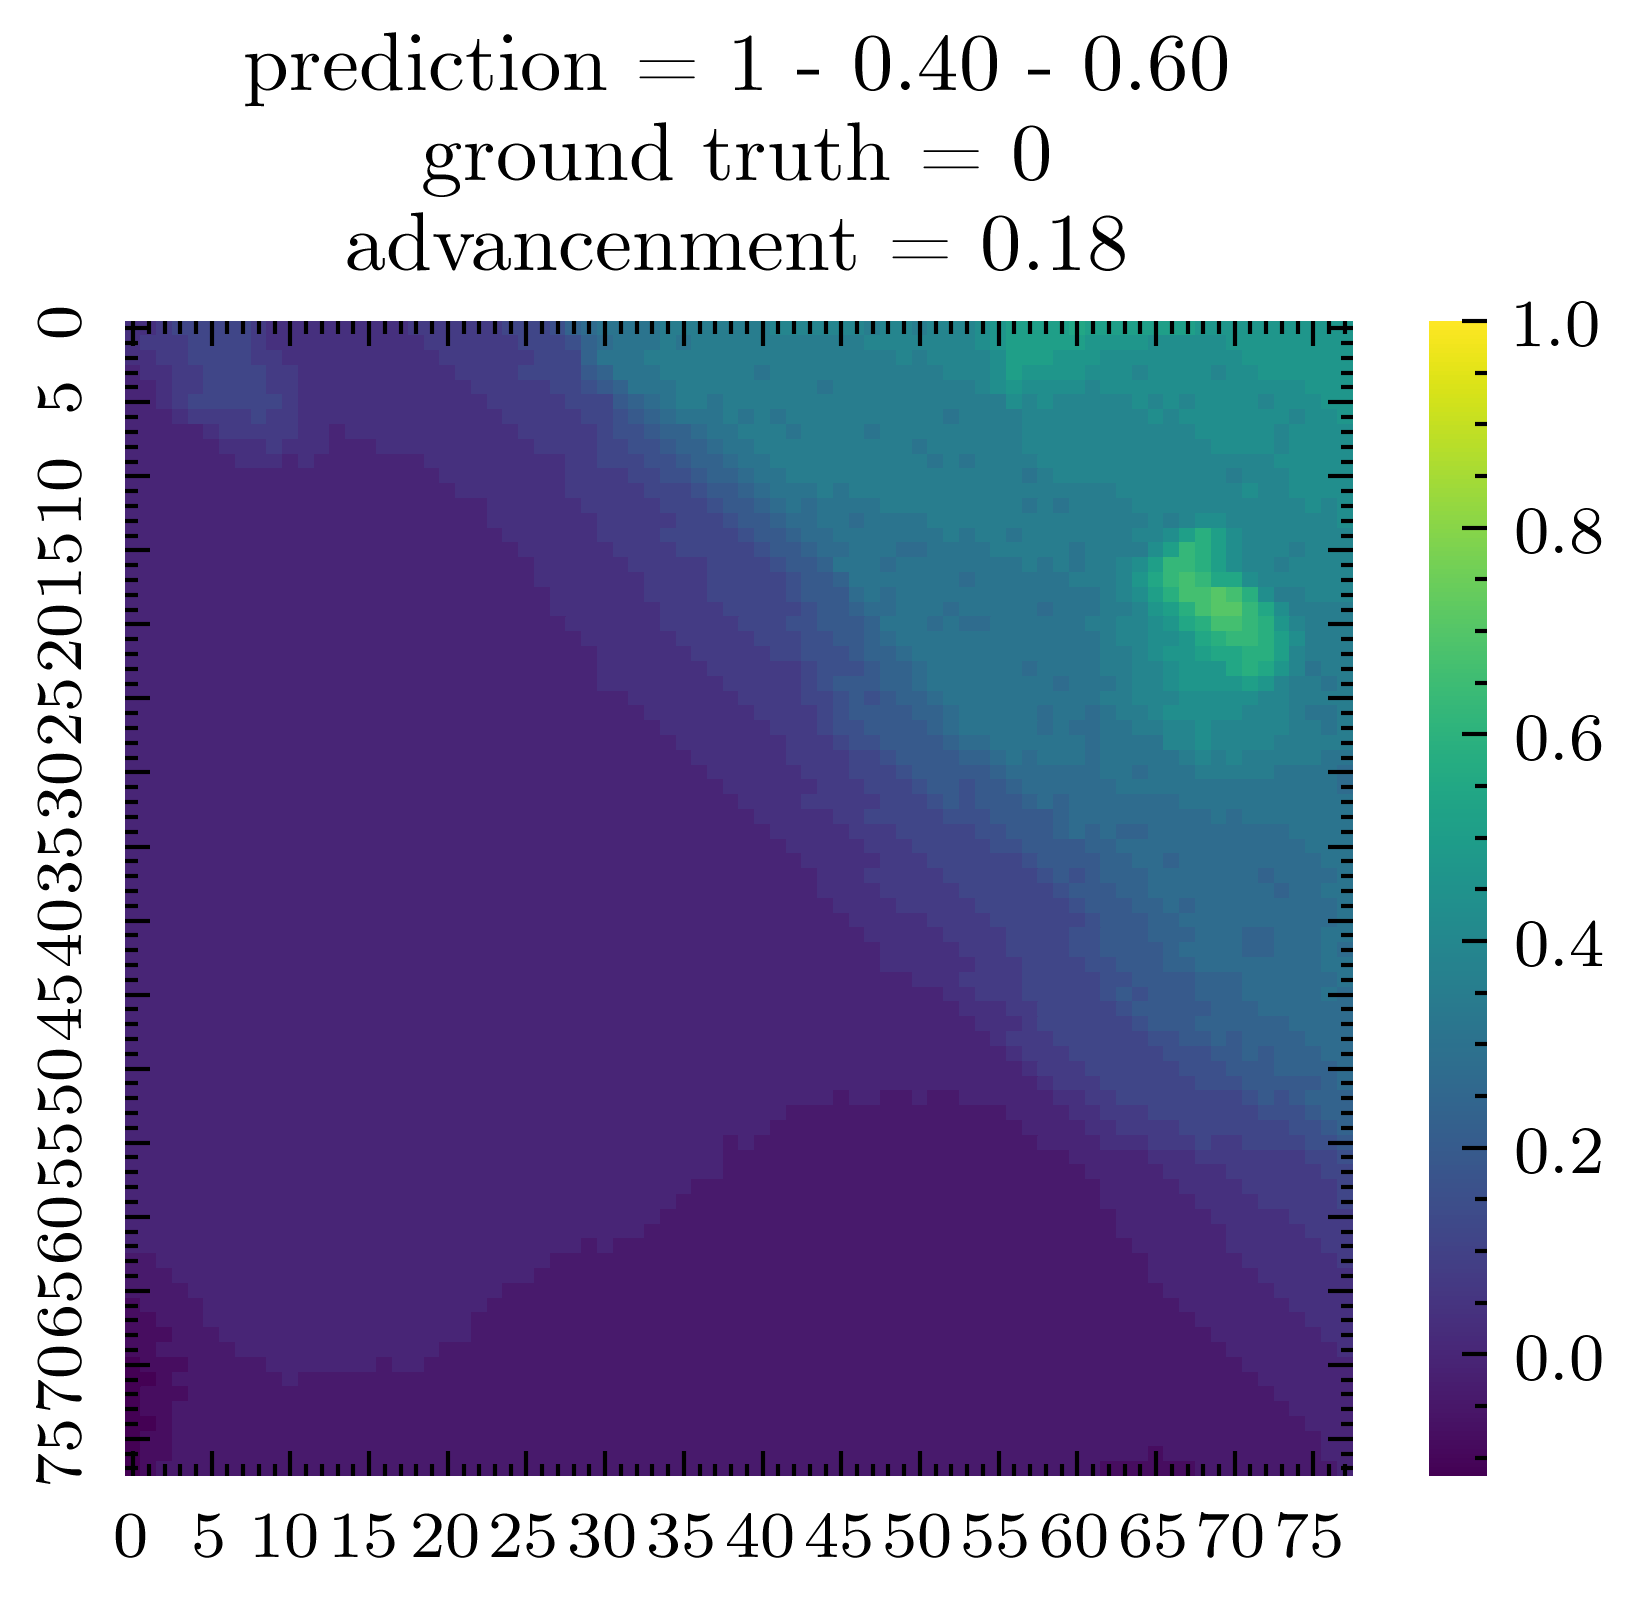
\includegraphics[width=\linewidth]{../img/5/quarry/worst/patch-2d-0.png}
    \end{subfigure}
    \begin{subfigure}[b]{0.19\textwidth}
        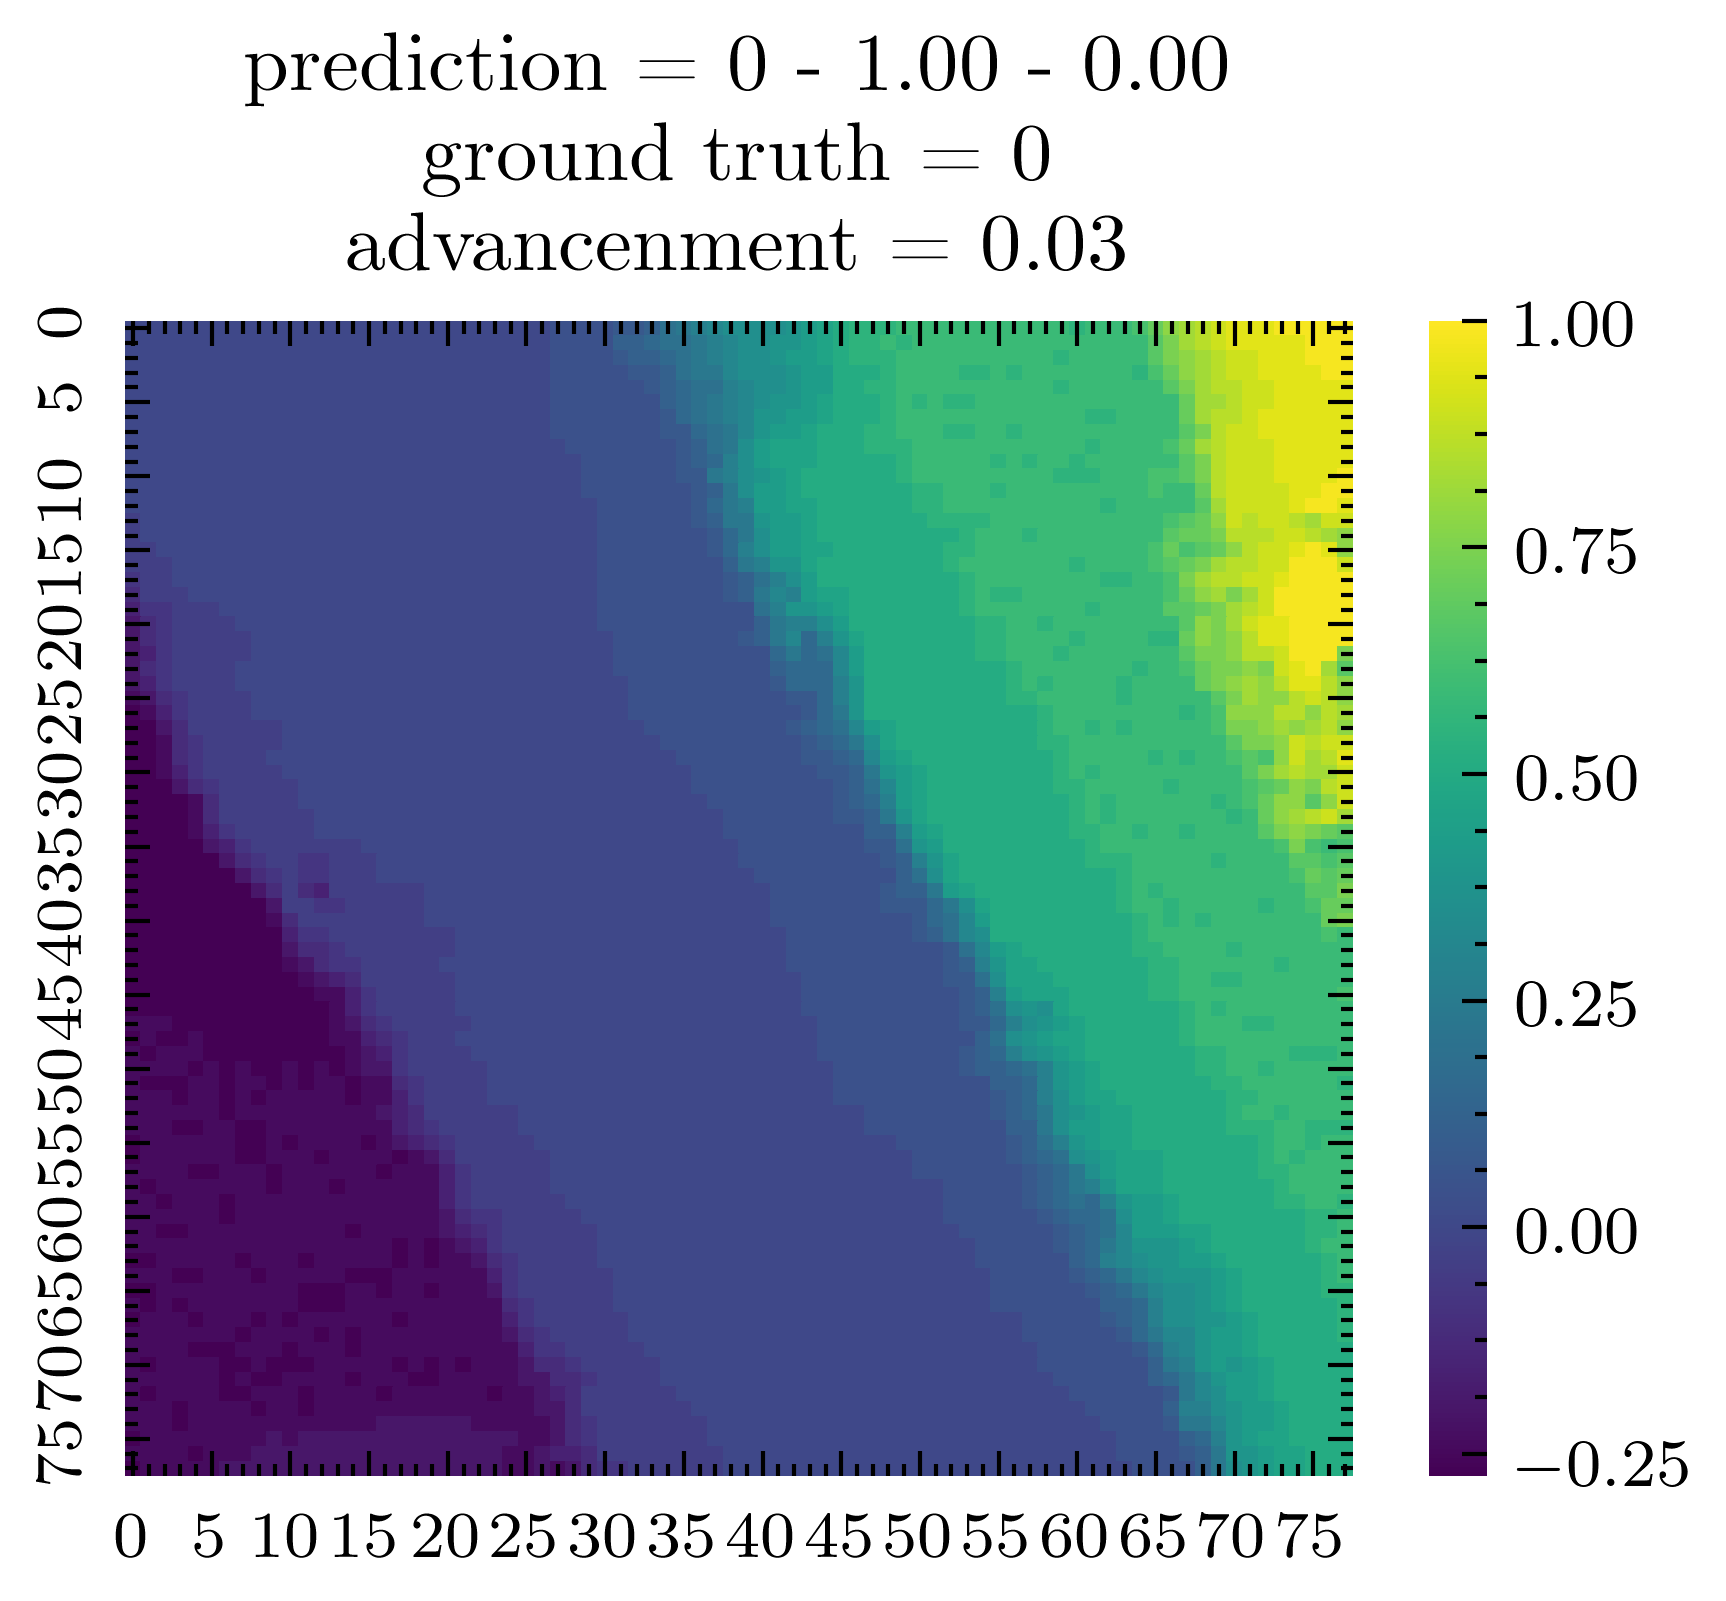
\includegraphics[width=\linewidth]{../img/5/quarry/worst/patch-2d-1.png}
    \end{subfigure}  
    \begin{subfigure}[b]{0.19\textwidth}
        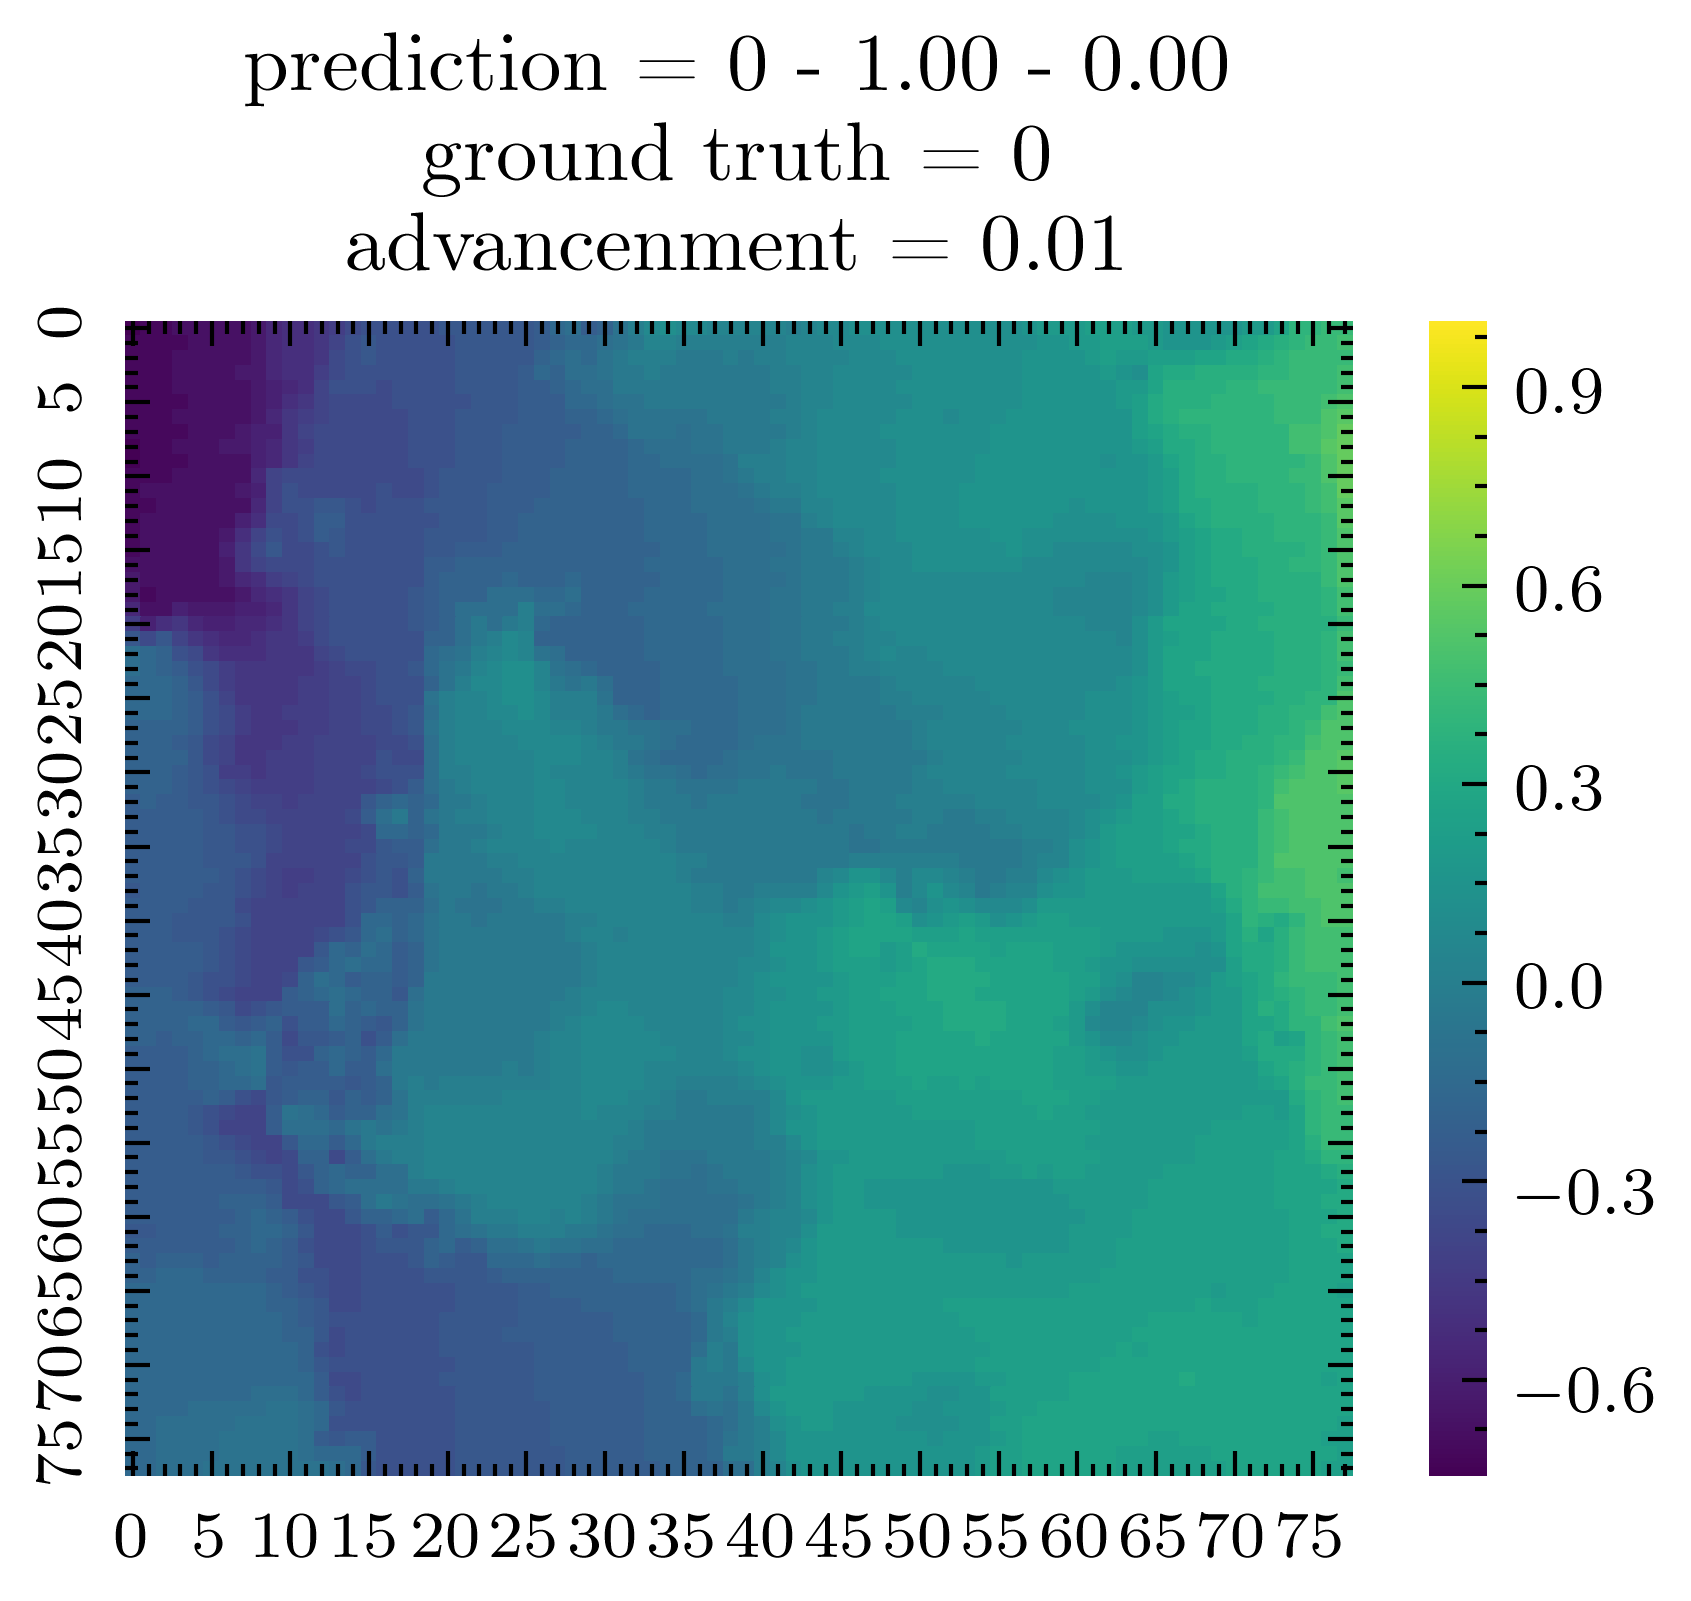
\includegraphics[width=\linewidth]{../img/5/quarry/worst/patch-2d-2.png}
    \end{subfigure}
    \begin{subfigure}[b]{0.19\textwidth}
        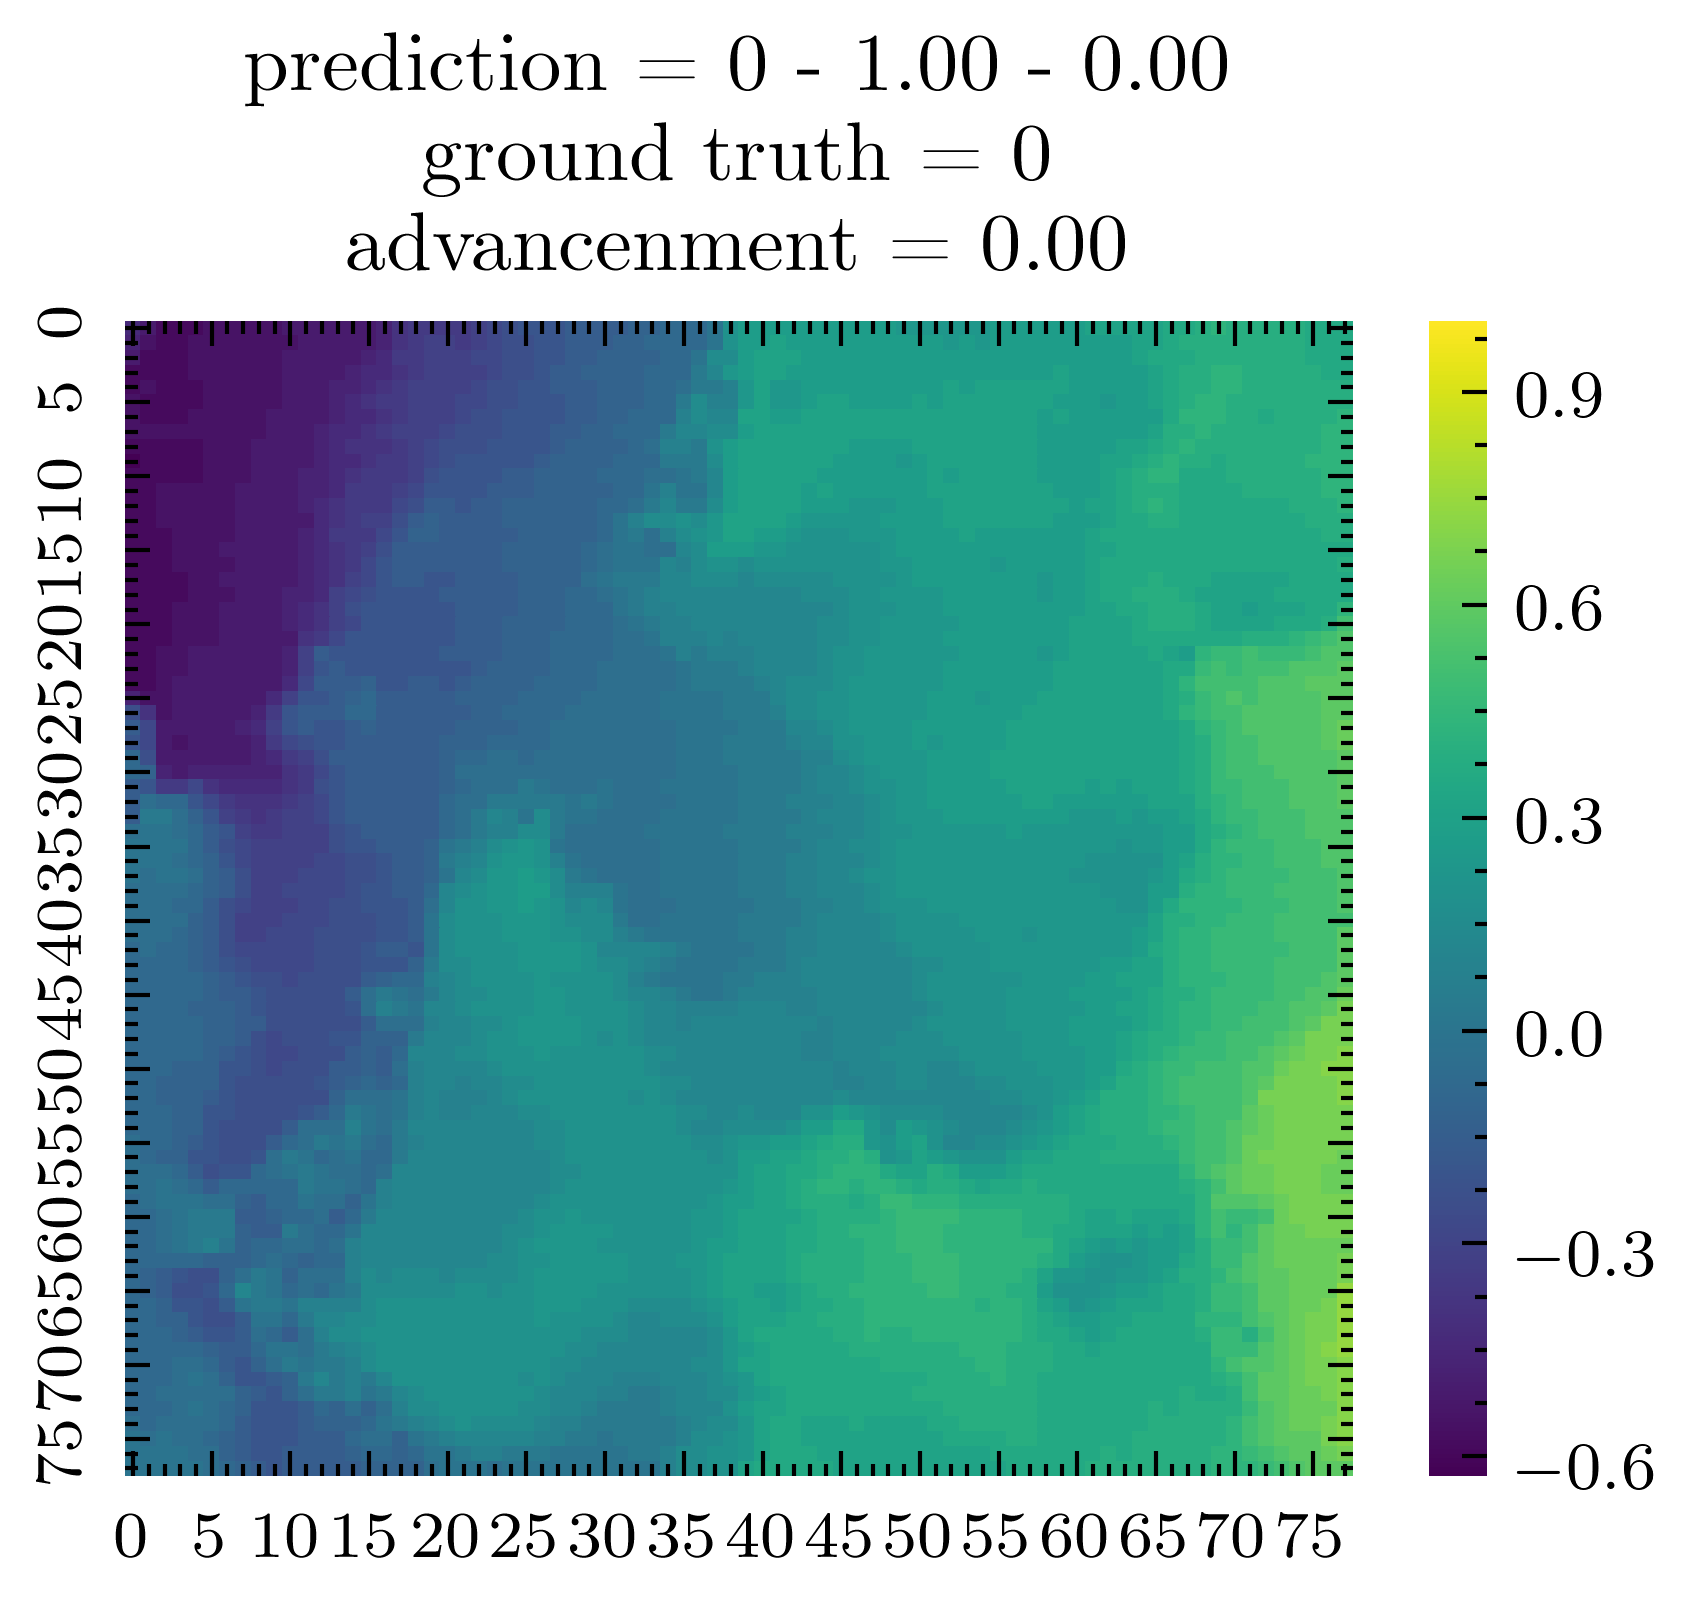
\includegraphics[width=\linewidth]{../img/5/quarry/worst/patch-2d-3.png}
    \end{subfigure}  
    \begin{subfigure}[b]{0.19\textwidth}
        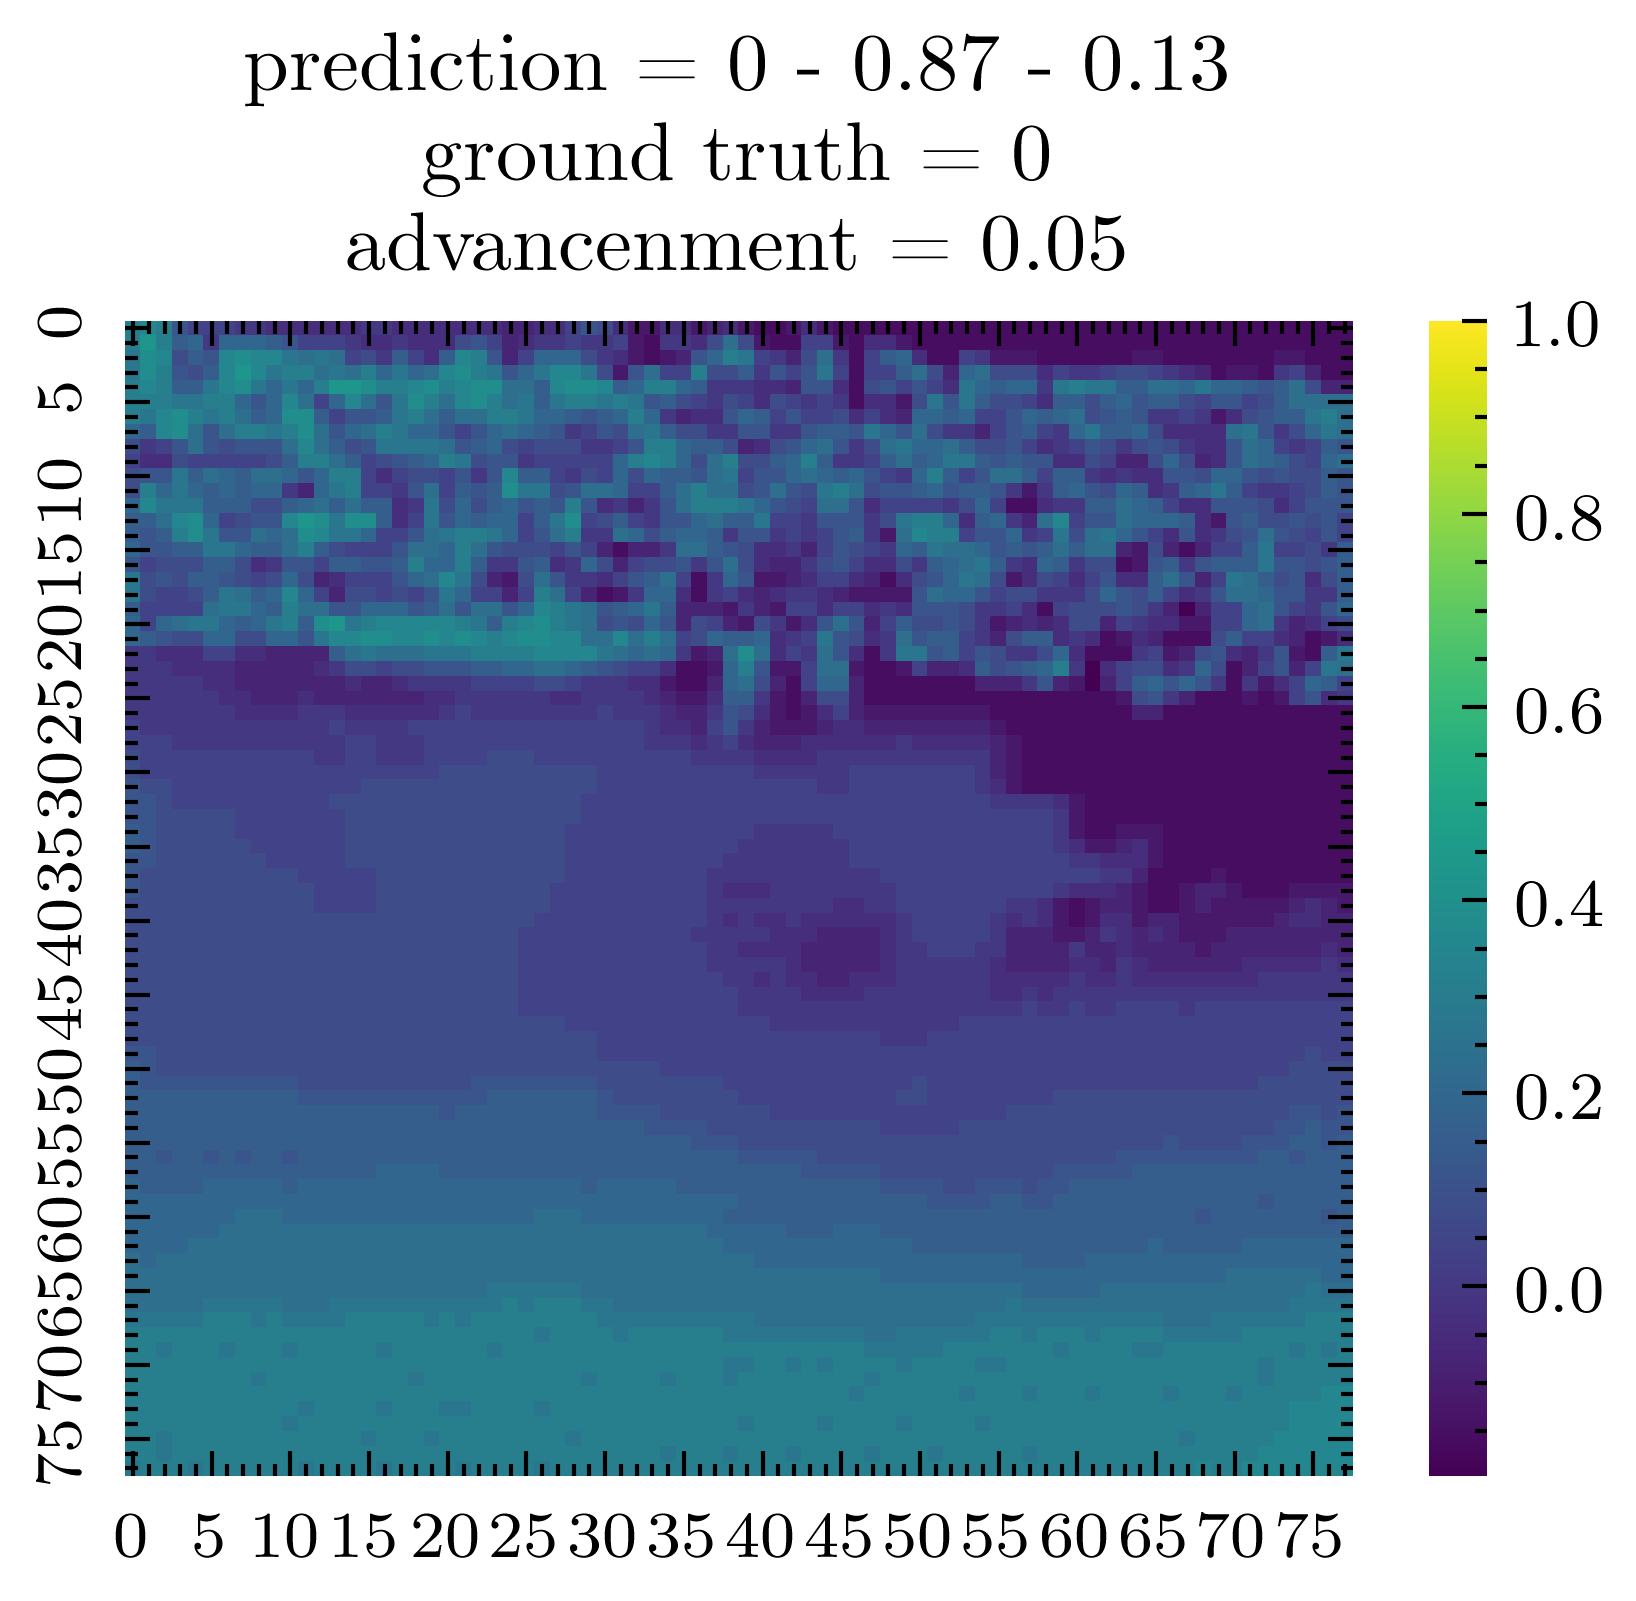
\includegraphics[width=\linewidth]{../img/5/quarry/worst/patch-2d-4.png}
    \end{subfigure}  

    \begin{subfigure}[b]{0.19\textwidth}
        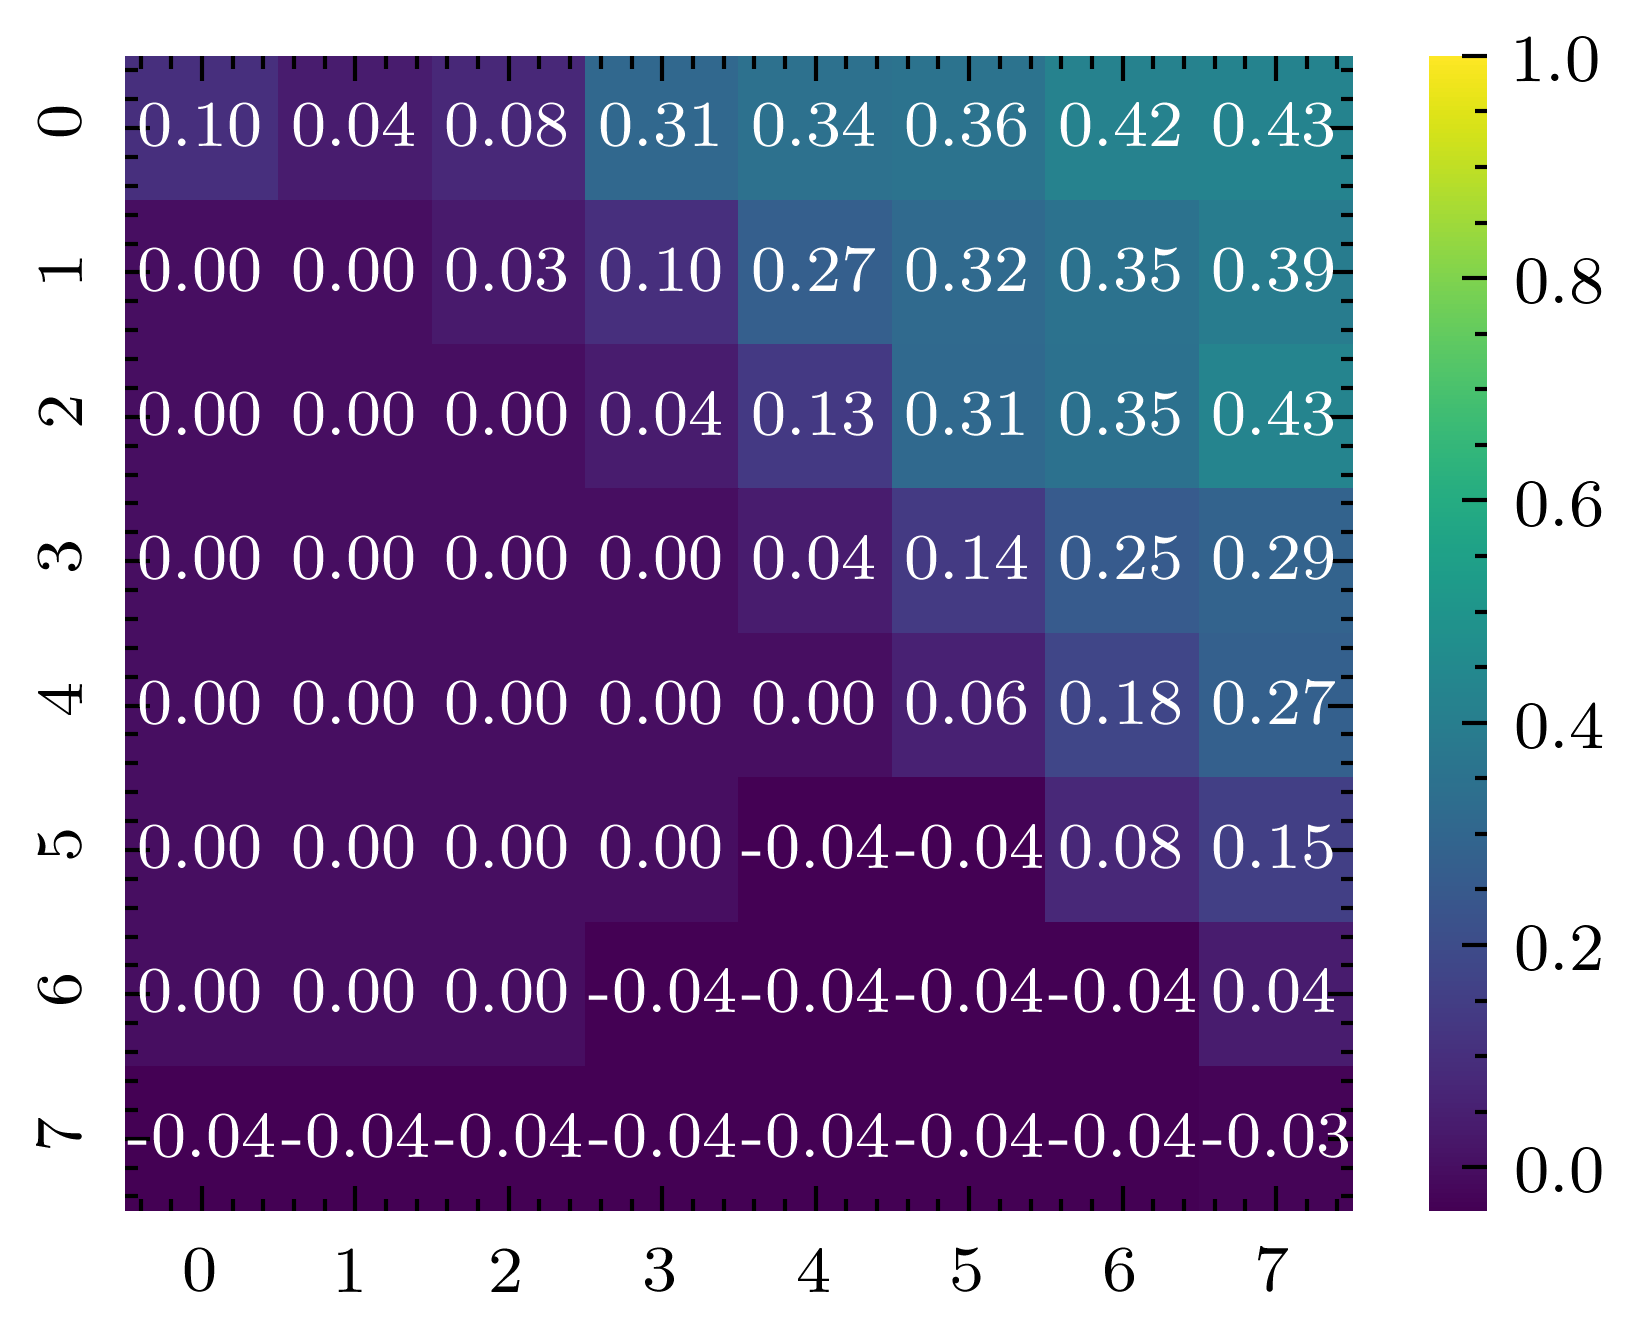
\includegraphics[width=\linewidth]{../img/5/quarry/worst/heatmap-2d-0.png}
    \end{subfigure}
    \begin{subfigure}[b]{0.19\textwidth}
        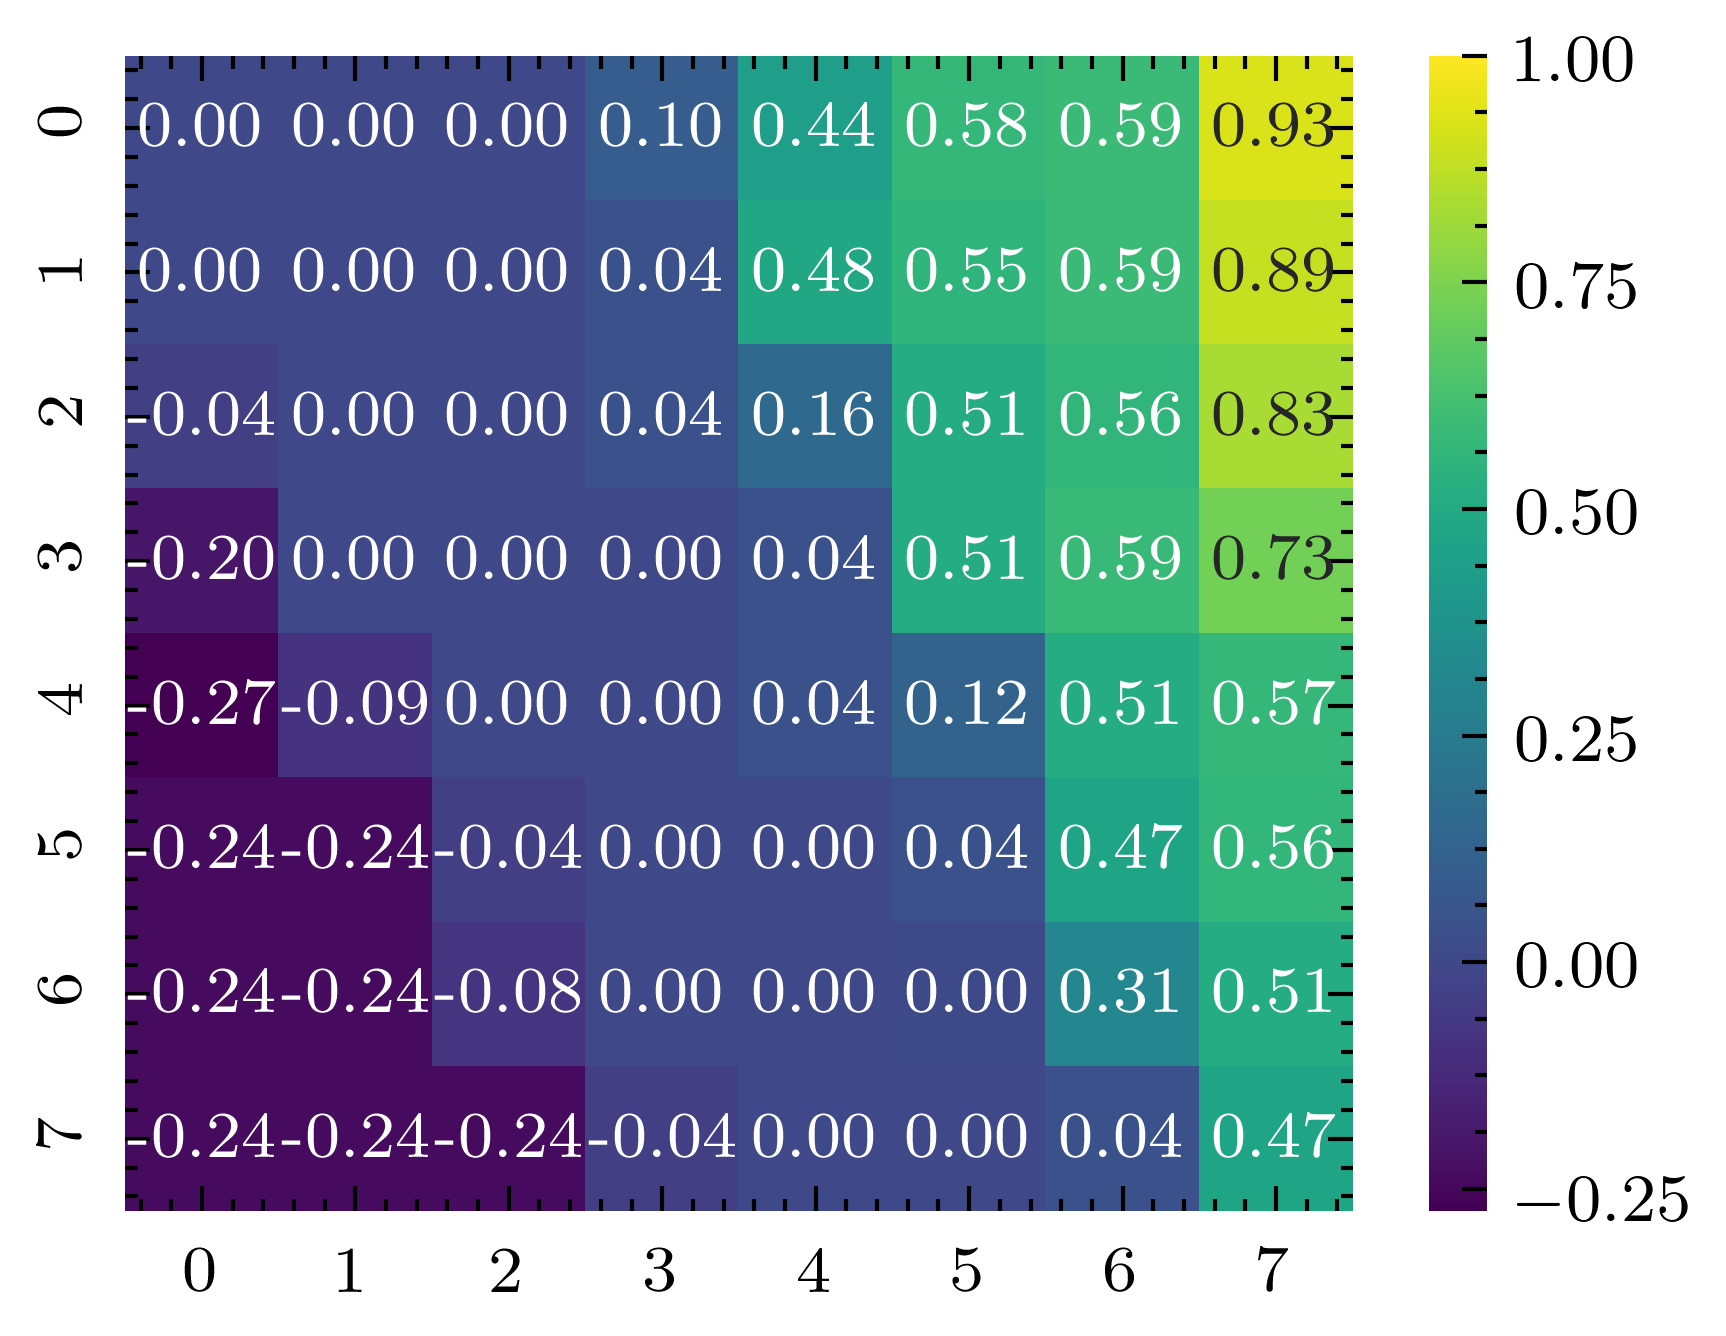
\includegraphics[width=\linewidth]{../img/5/quarry/worst/heatmap-2d-1.png}
    \end{subfigure}  
    \begin{subfigure}[b]{0.19\textwidth}
        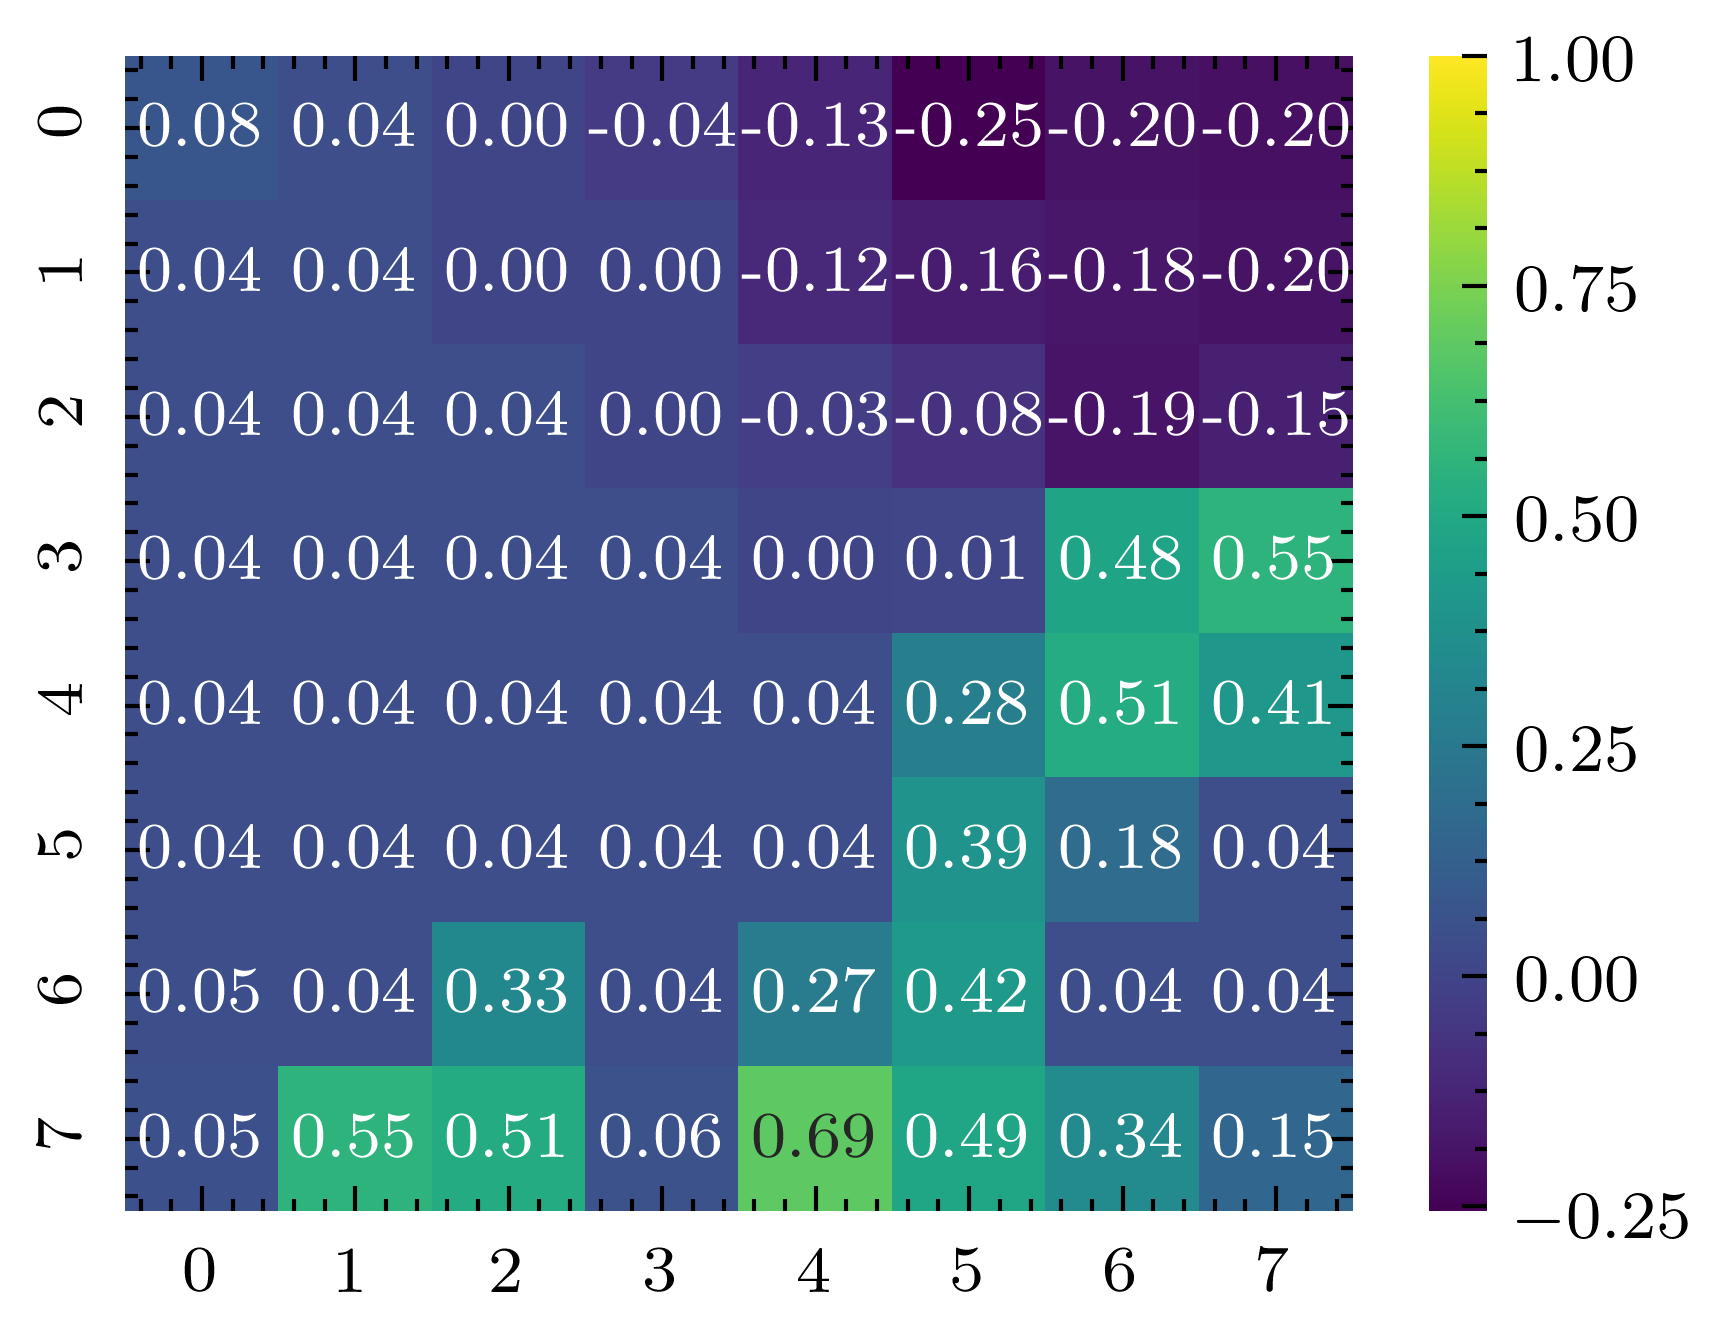
\includegraphics[width=\linewidth]{../img/5/quarry/worst/heatmap-2d-2.png}
    \end{subfigure}
    \begin{subfigure}[b]{0.19\textwidth}
        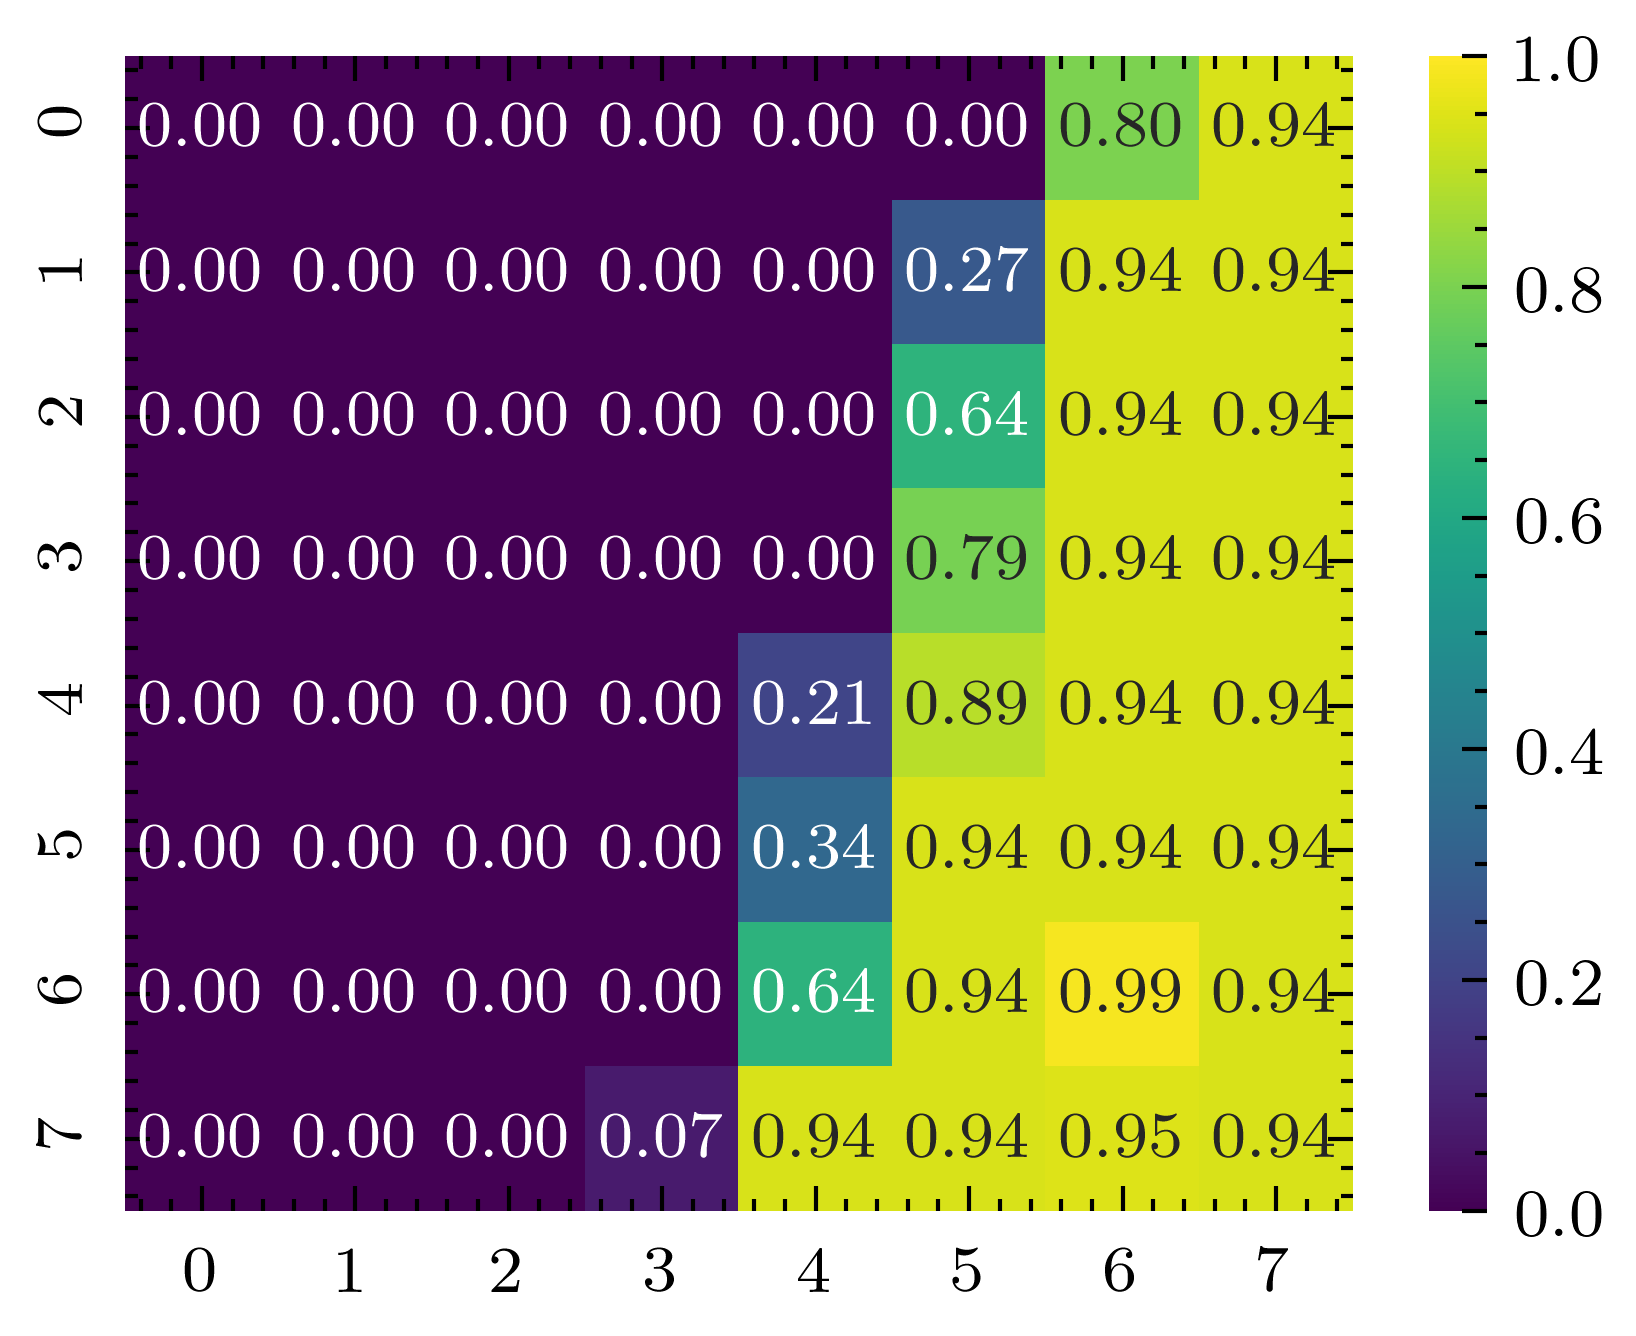
\includegraphics[width=\linewidth]{../img/5/quarry/worst/heatmap-2d-3.png}
    \end{subfigure}  
    \begin{subfigure}[b]{0.19\textwidth}
        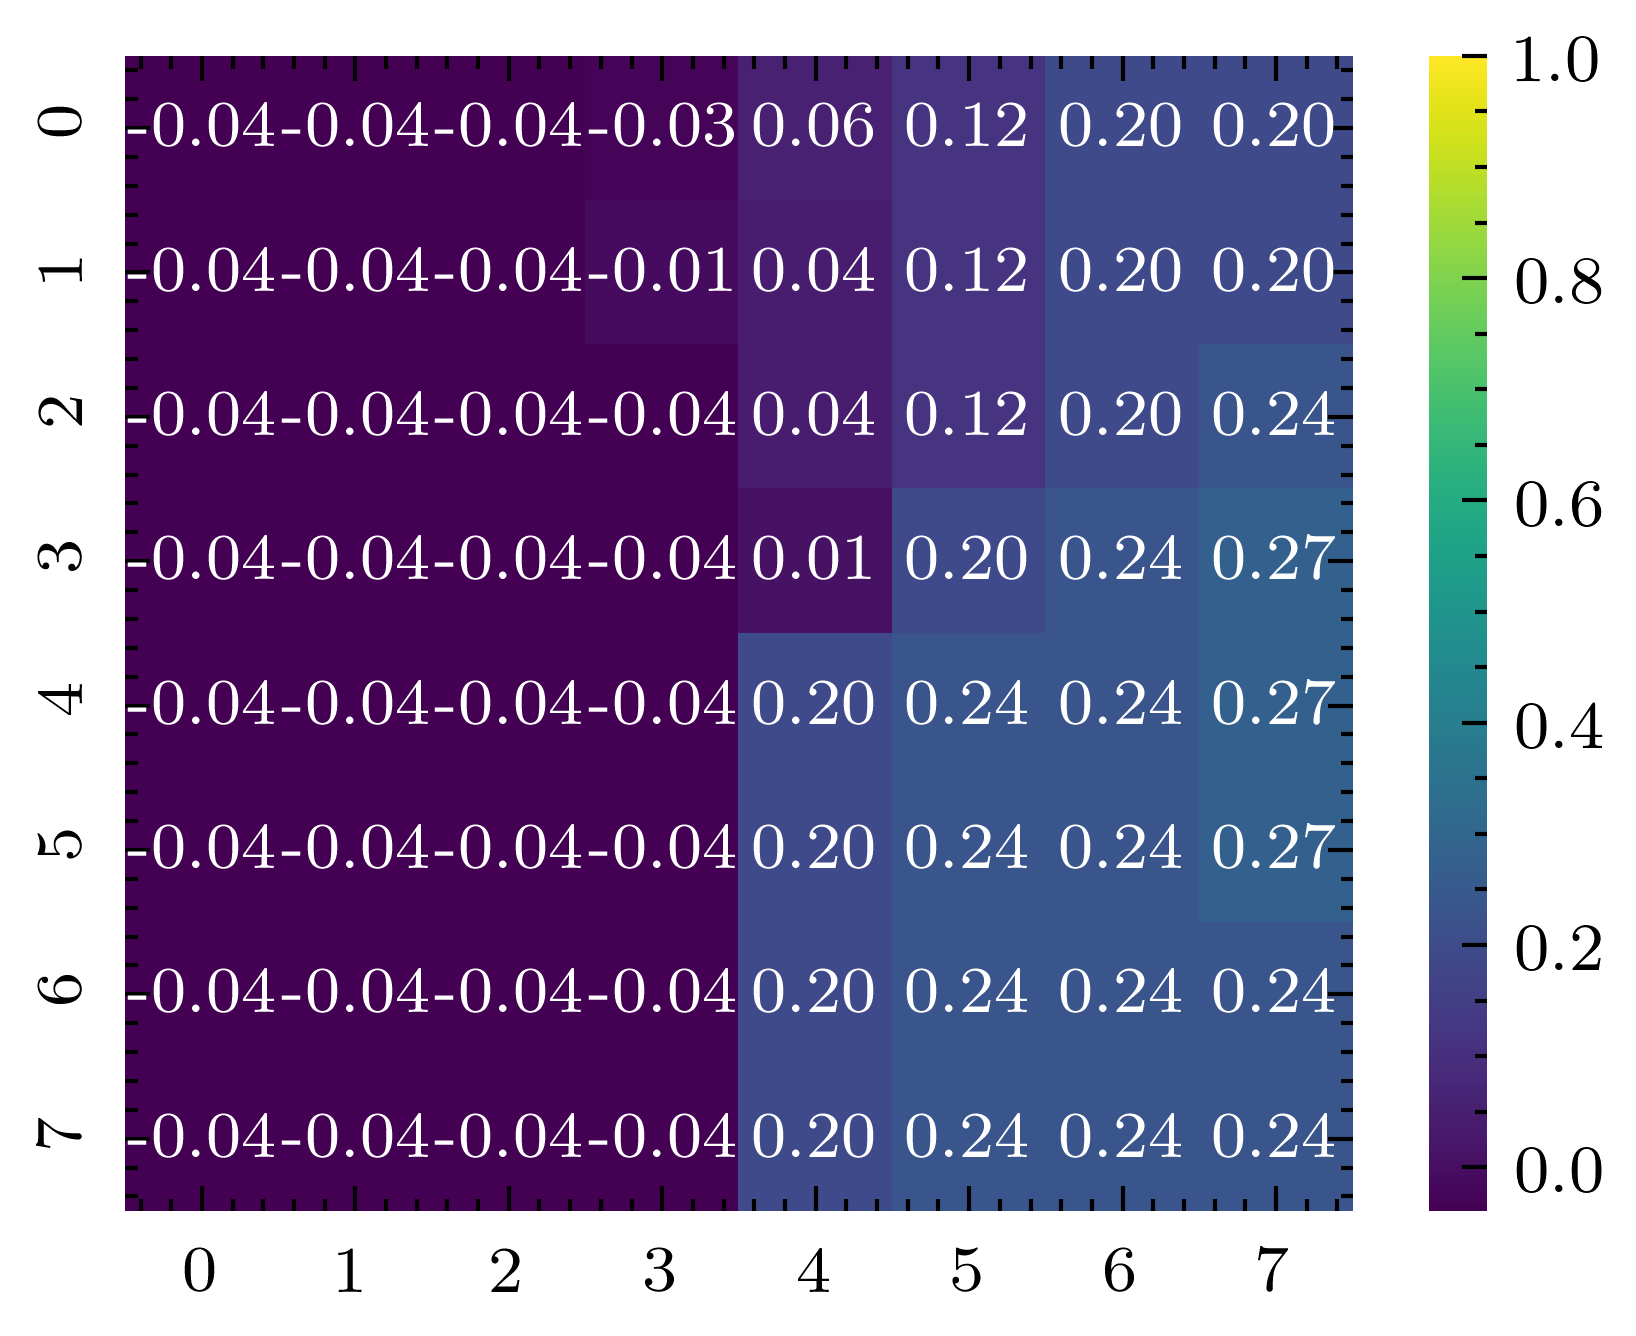
\includegraphics[width=\linewidth]{../img/5/quarry/worst/heatmap-2d-4.png}
    \end{subfigure}  

    \begin{subfigure}[b]{0.19\textwidth}
        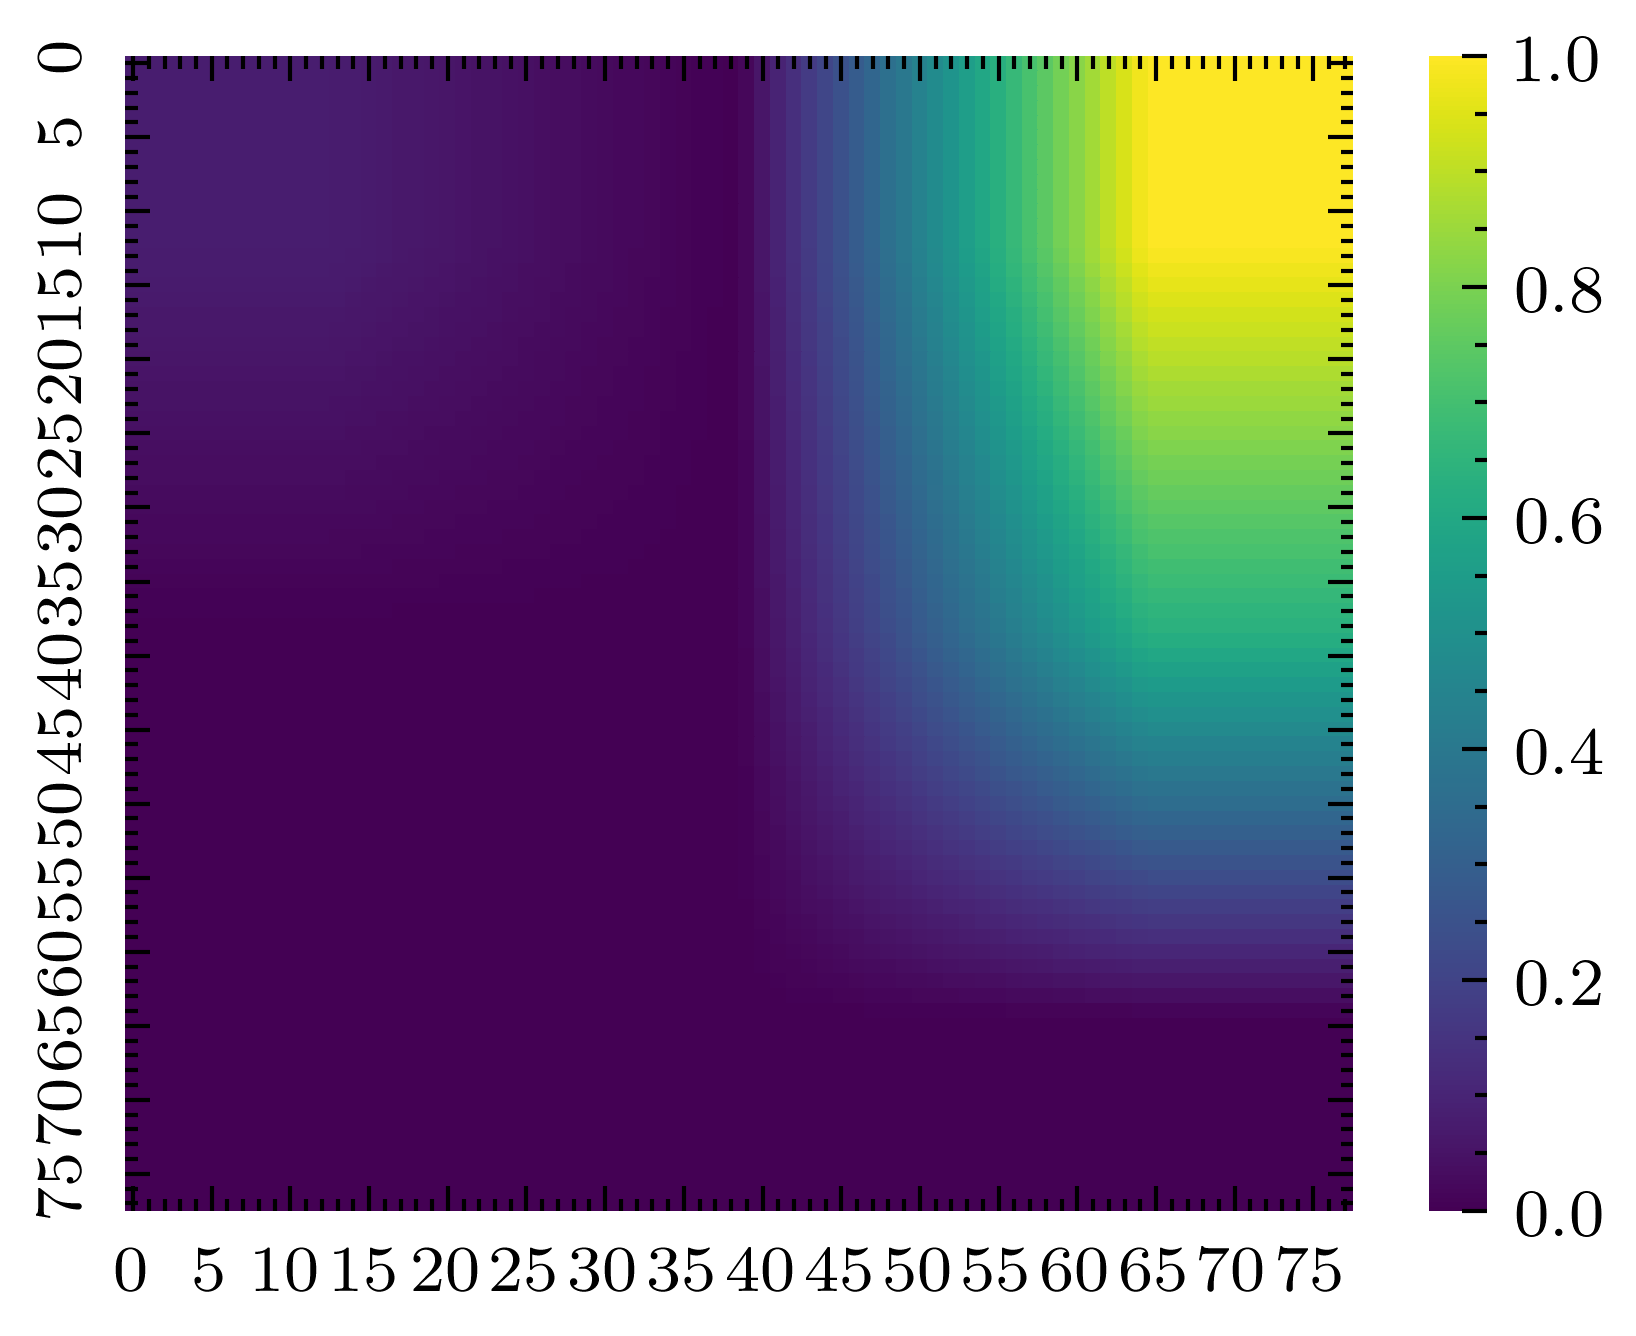
\includegraphics[width=\linewidth]{../img/5/quarry/worst/grad-cam-2d-0.png}
    \end{subfigure}
    \begin{subfigure}[b]{0.19\textwidth}
        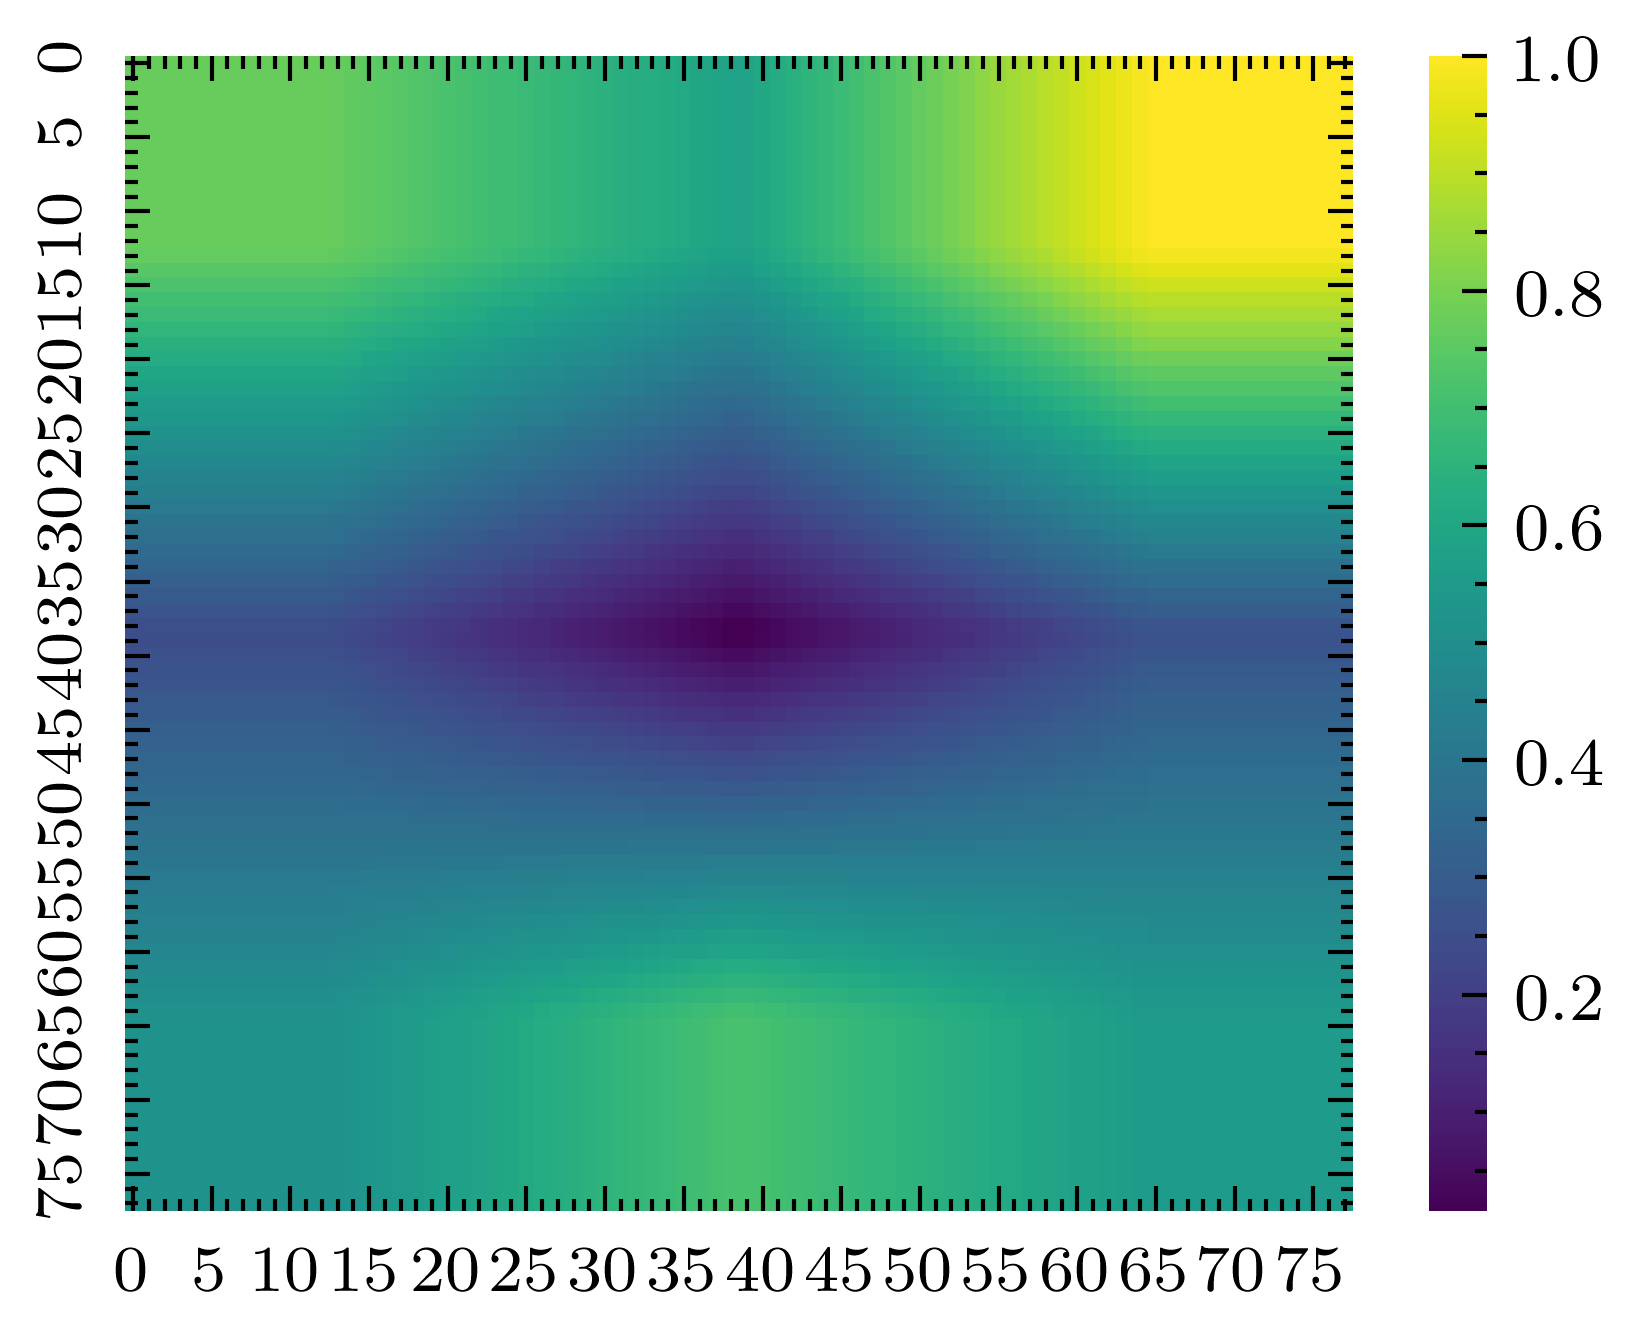
\includegraphics[width=\linewidth]{../img/5/quarry/worst/grad-cam-2d-1.png}
    \end{subfigure}  
    \begin{subfigure}[b]{0.19\textwidth}
        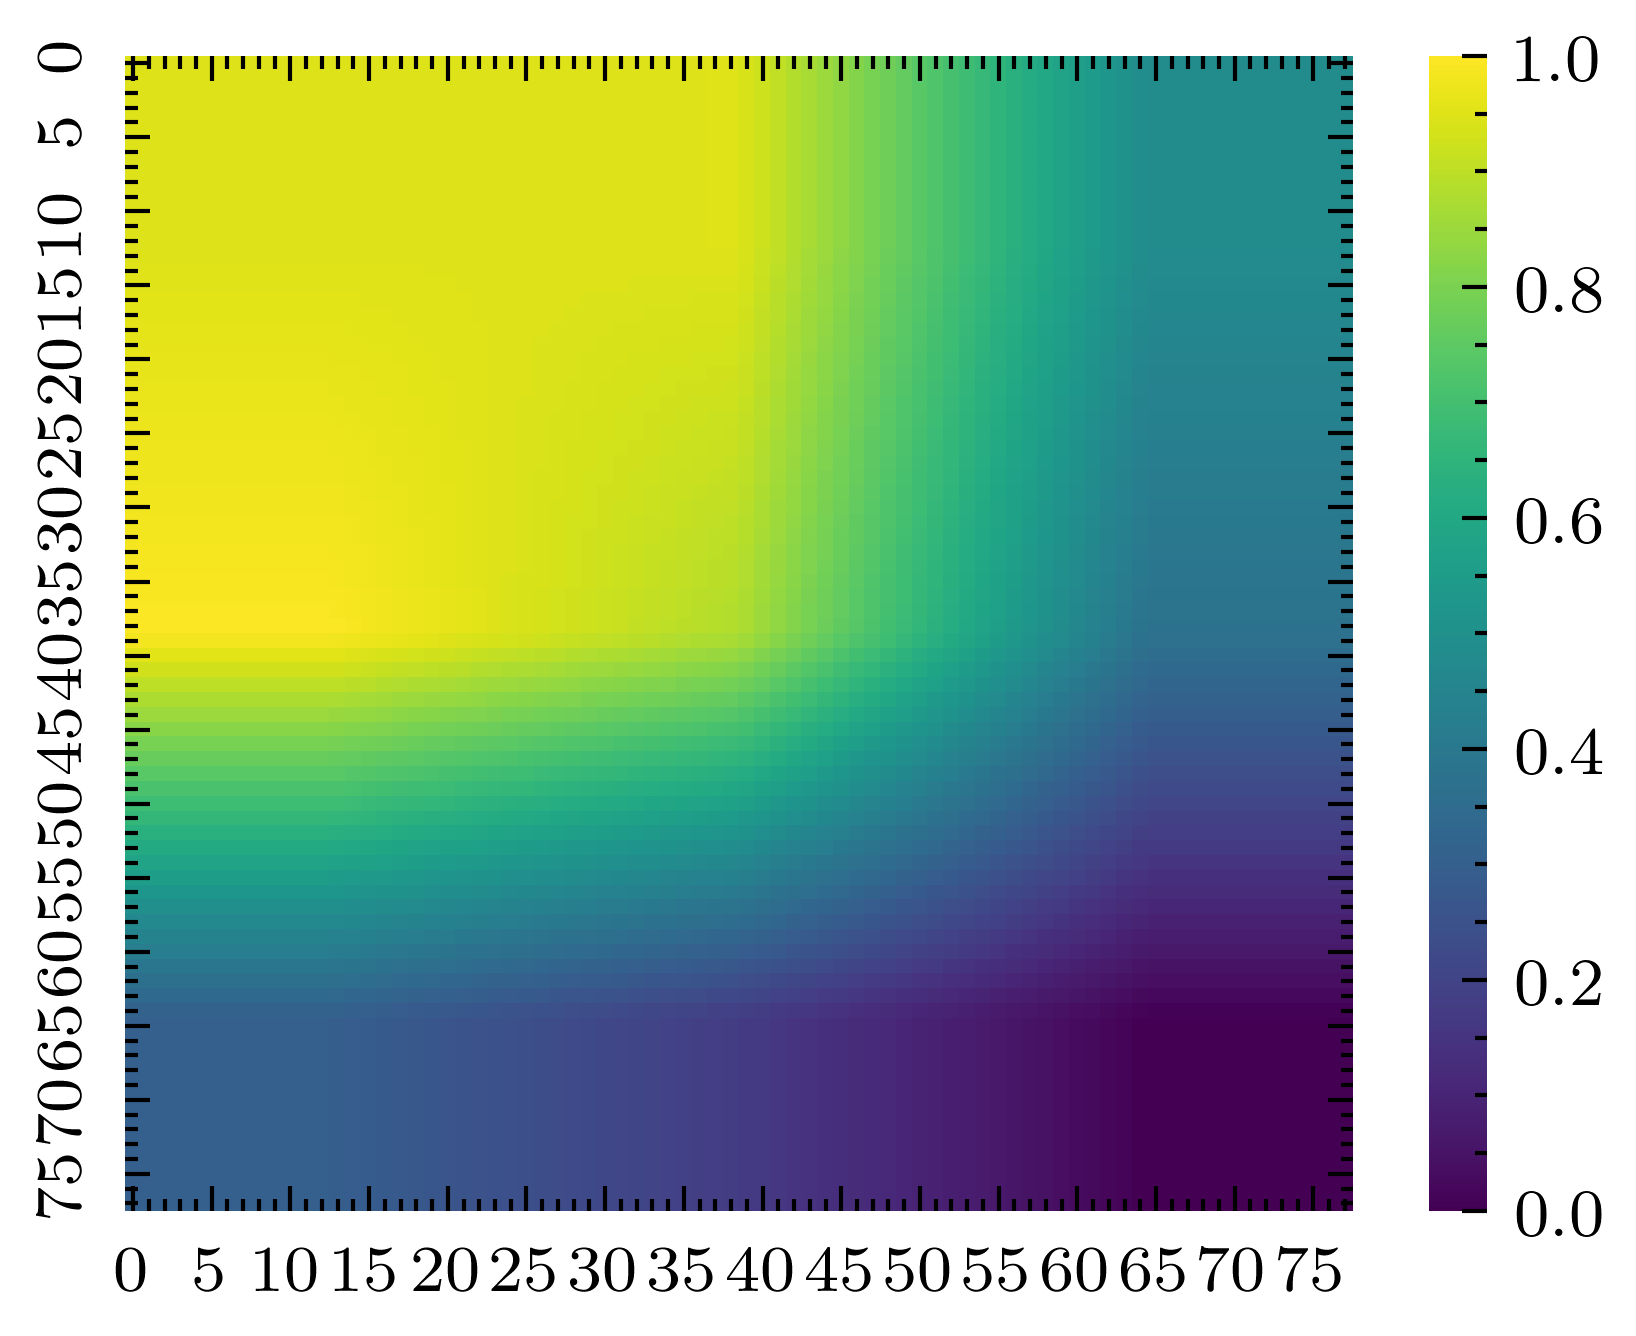
\includegraphics[width=\linewidth]{../img/5/quarry/worst/grad-cam-2d-2.png}
    \end{subfigure}
    \begin{subfigure}[b]{0.19\textwidth}
        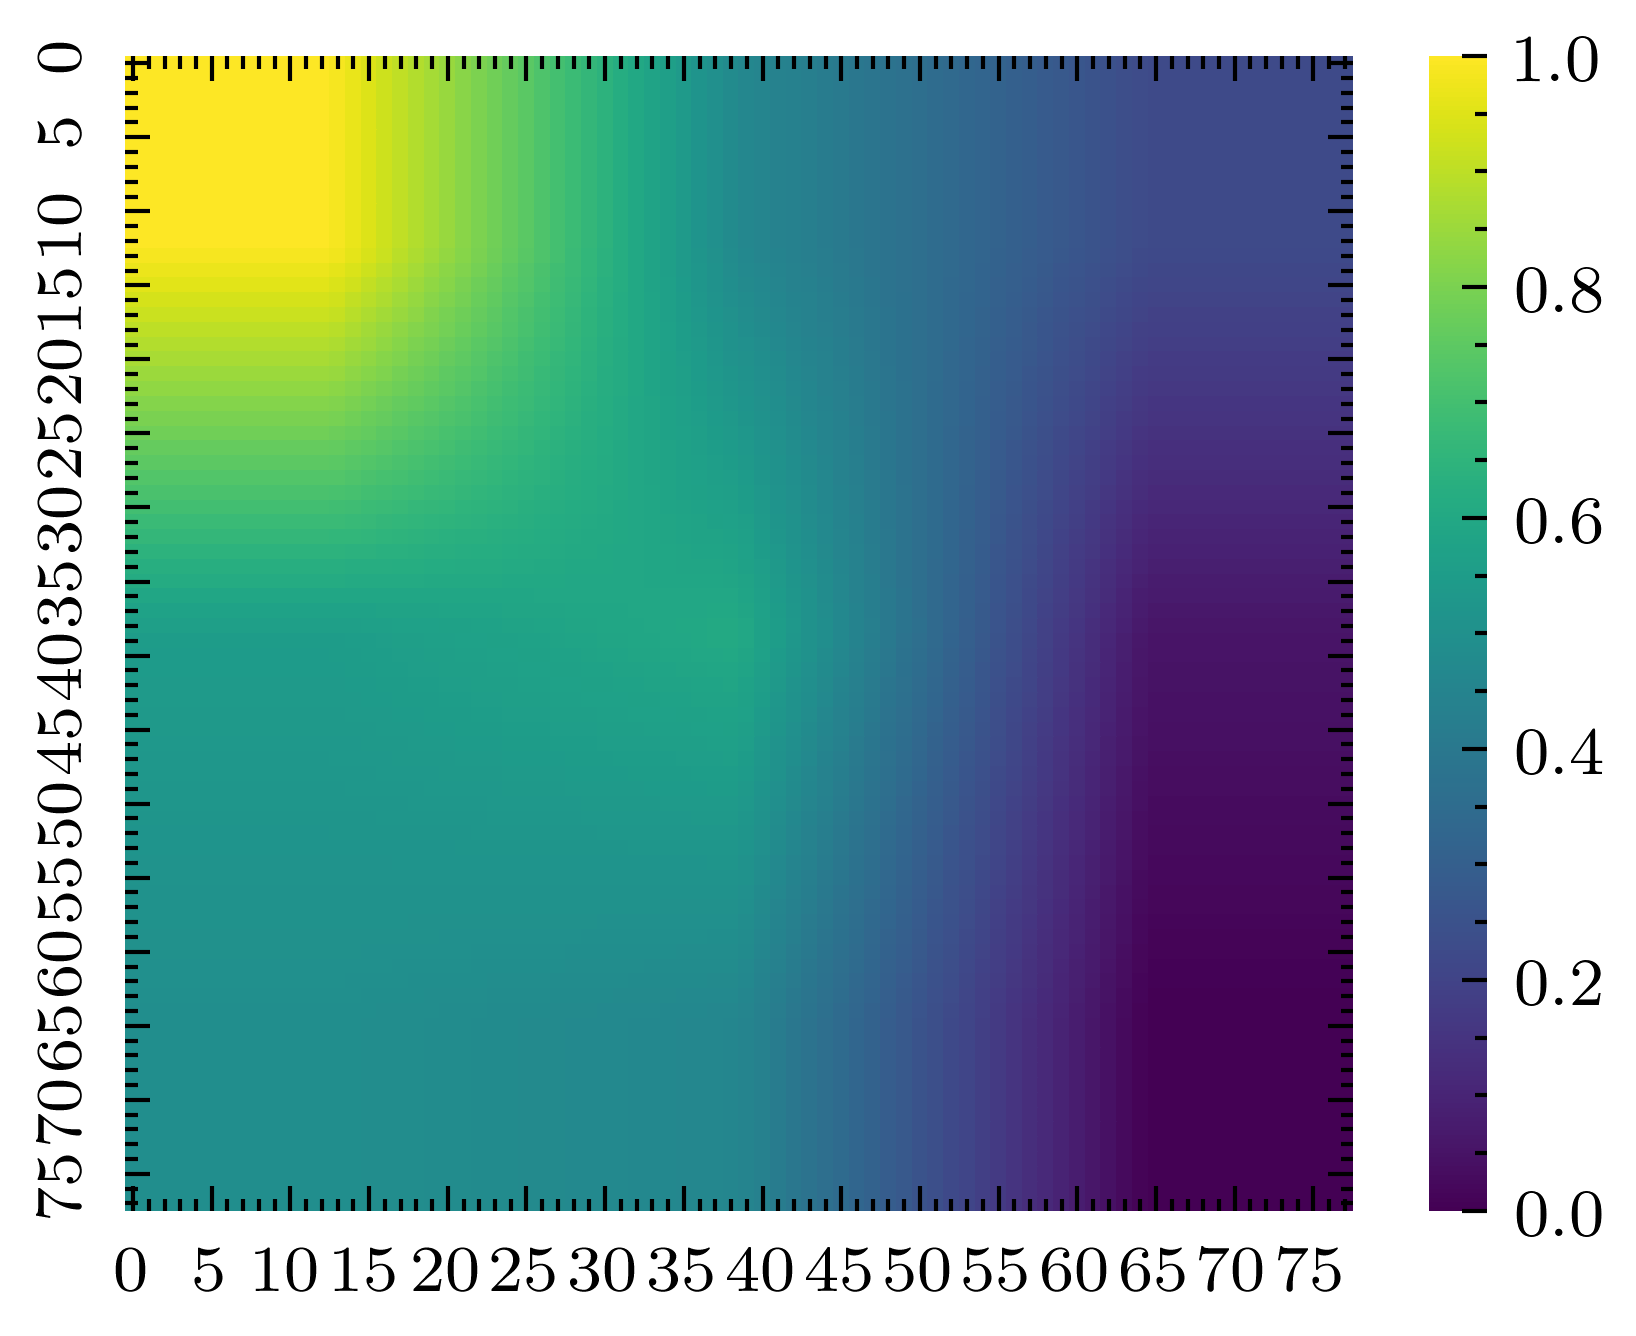
\includegraphics[width=\linewidth]{../img/5/quarry/worst/grad-cam-2d-3.png}
    \end{subfigure}  
    \begin{subfigure}[b]{0.19\textwidth}
        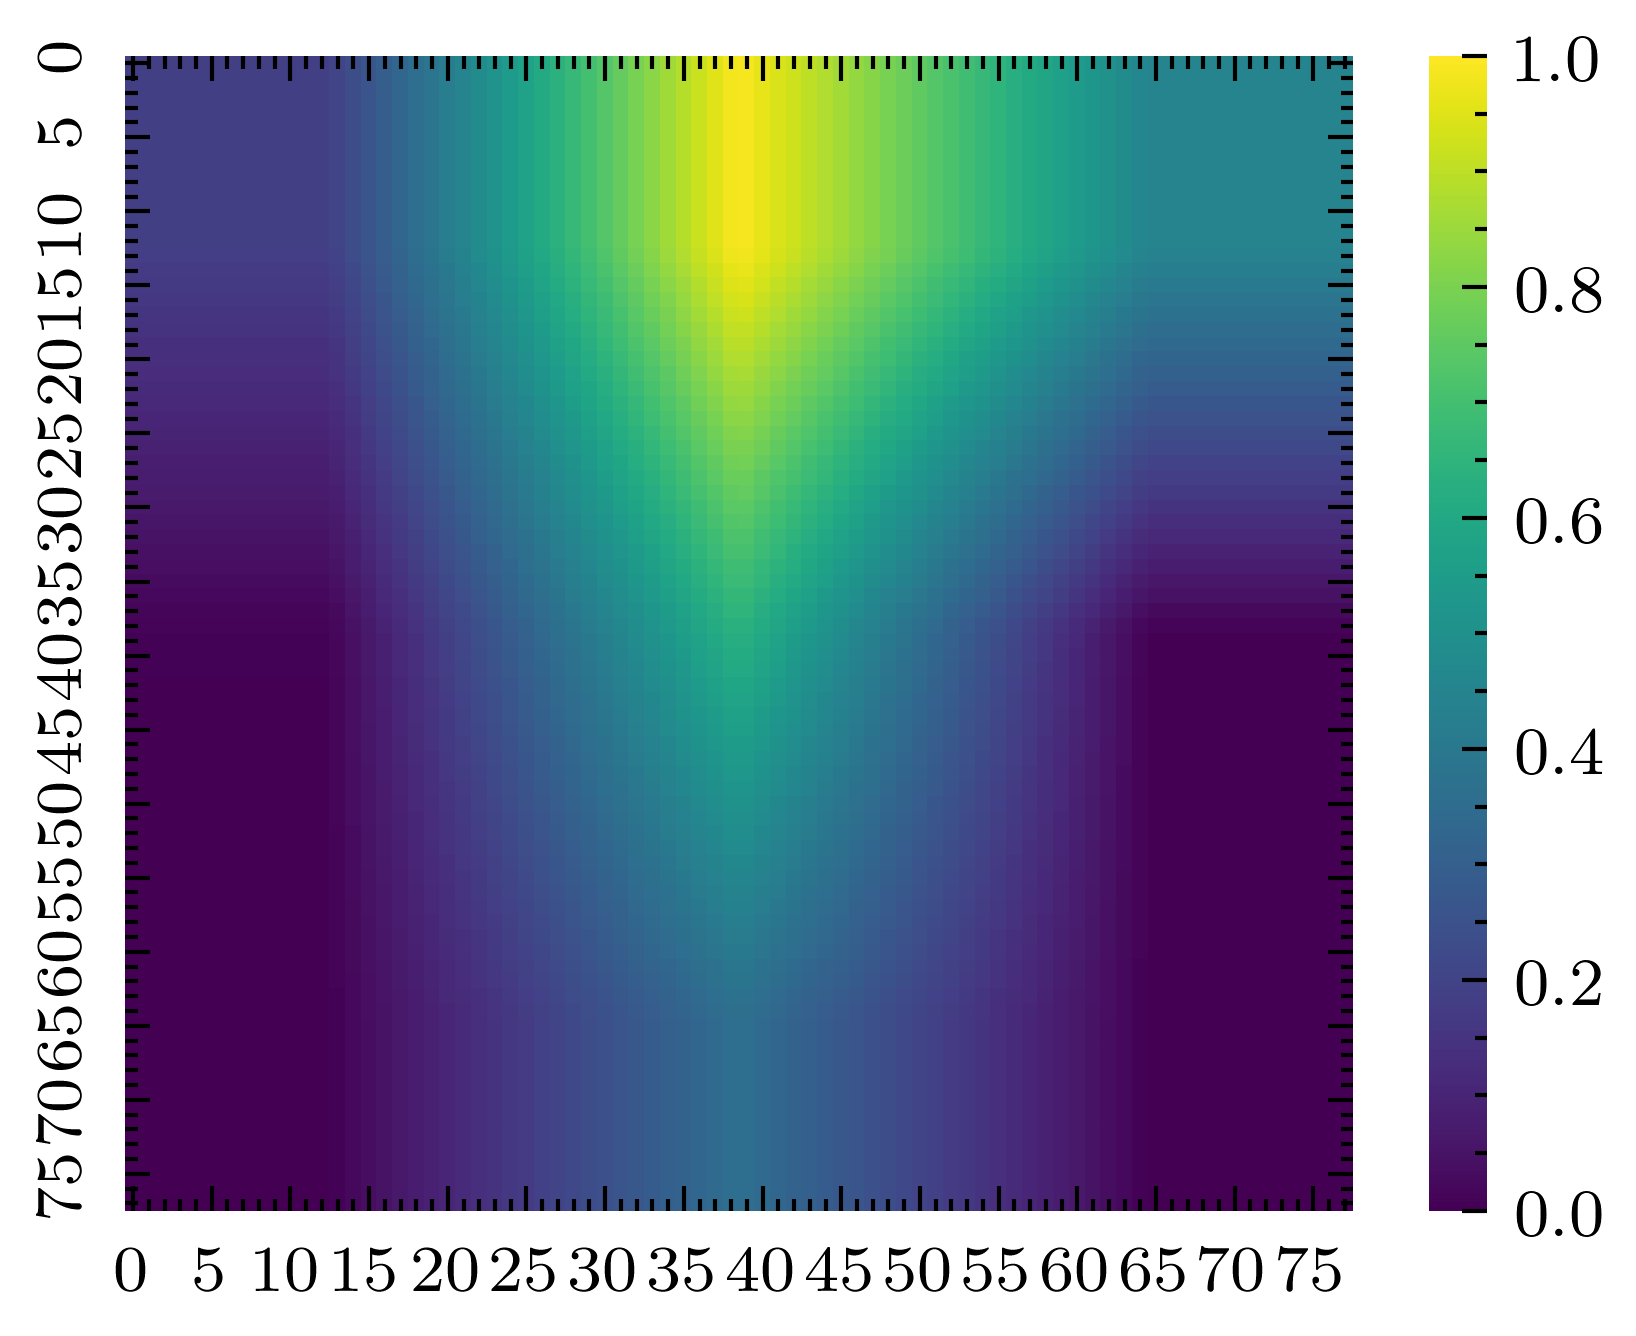
\includegraphics[width=\linewidth]{../img/5/quarry/worst/grad-cam-2d-4.png}
    \end{subfigure}  

    \begin{subfigure}[b]{0.19\textwidth}
        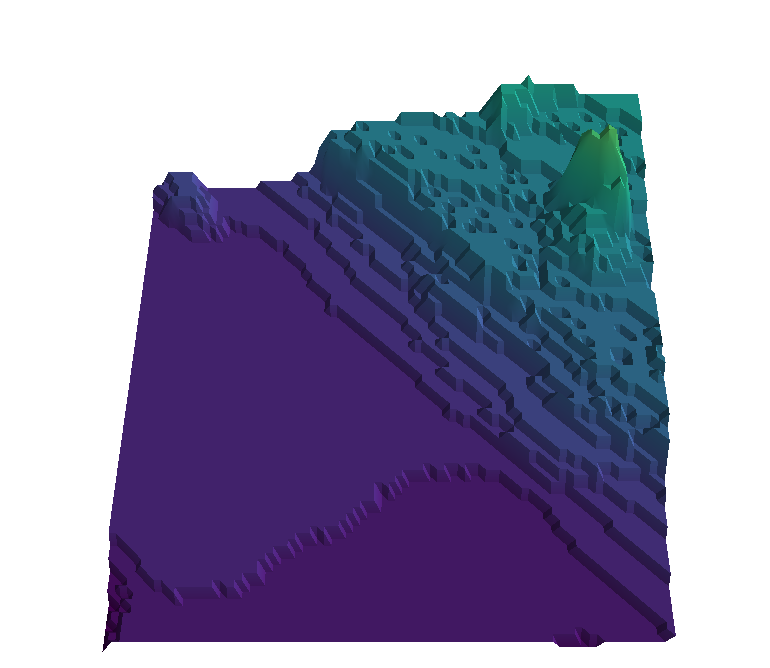
\includegraphics[width=\linewidth]{../img/5/quarry/worst//patch-3d-majavi-colormap-0.png}
    \end{subfigure}
    \begin{subfigure}[b]{0.19\textwidth}
        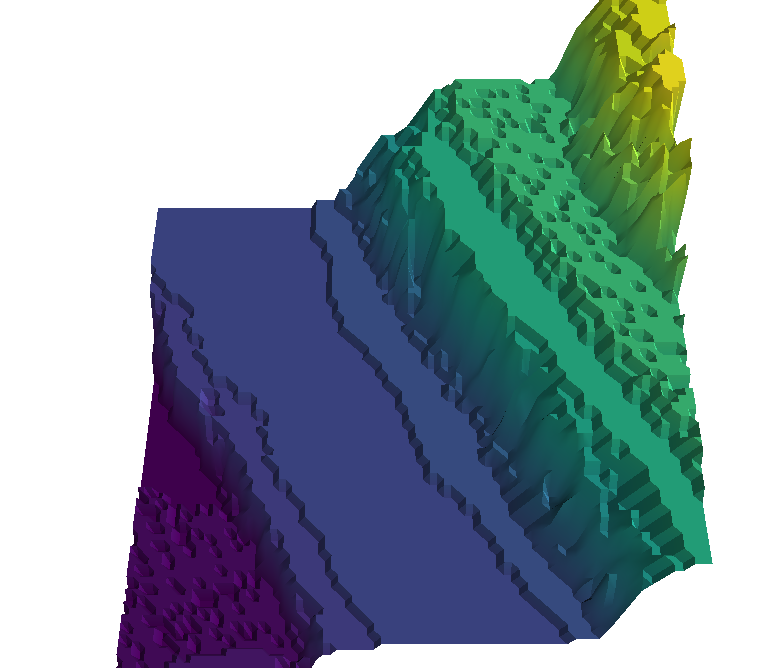
\includegraphics[width=\linewidth]{../img/5/quarry/worst//patch-3d-majavi-colormap-1.png}
    \end{subfigure}  
    \begin{subfigure}[b]{0.19\textwidth}
        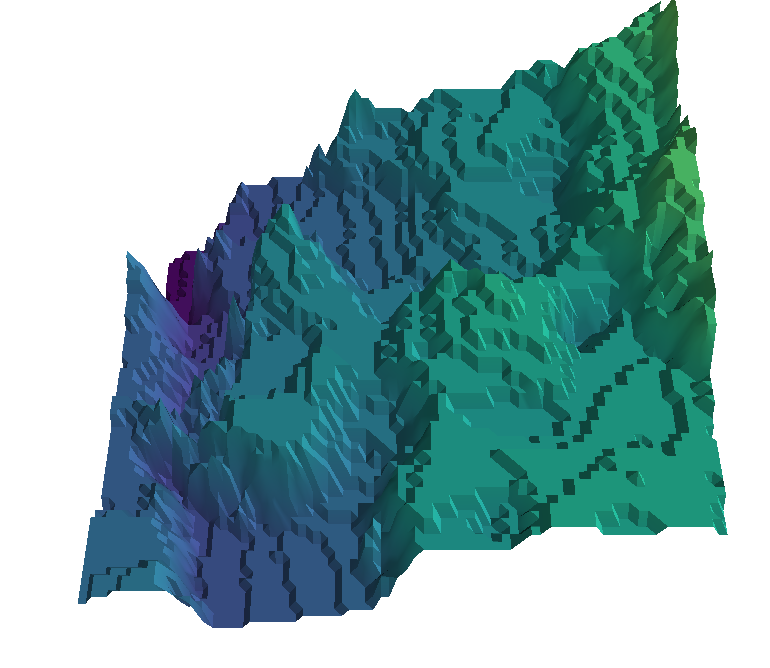
\includegraphics[width=\linewidth]{../img/5/quarry/worst//patch-3d-majavi-colormap-2.png}
    \end{subfigure}
    \begin{subfigure}[b]{0.19\textwidth}
        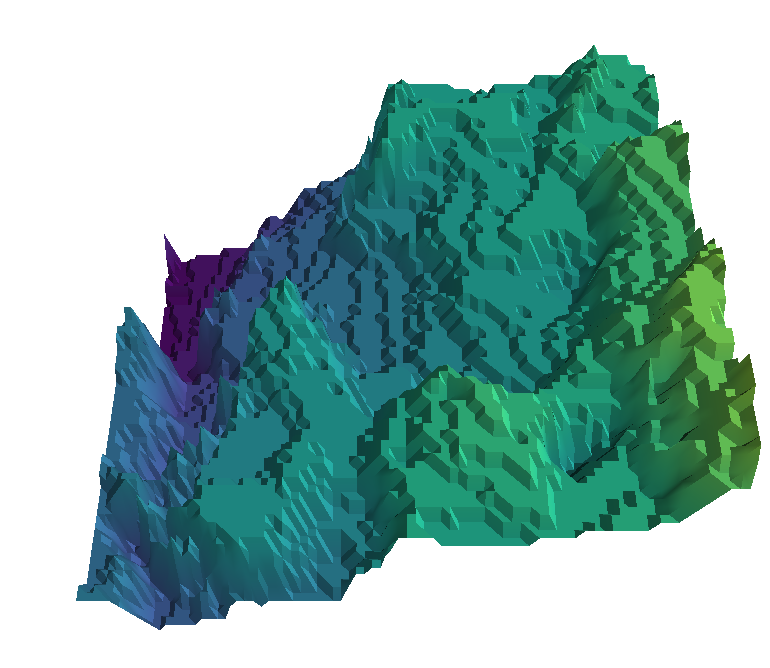
\includegraphics[width=\linewidth]{../img/5/quarry/worst//patch-3d-majavi-colormap-3.png}
    \end{subfigure}  
    \begin{subfigure}[b]{0.19\textwidth}
        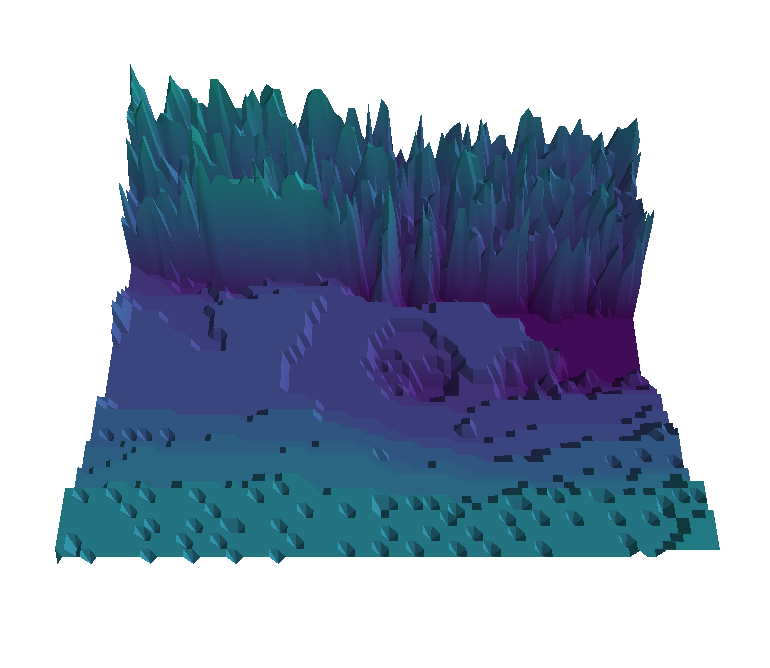
\includegraphics[width=\linewidth]{../img/5/quarry/worst//patch-3d-majavi-colormap-4.png}
    \end{subfigure}  

\caption{Worst}    
\end{figure}


\begin{figure}[H]
    \centering
    \begin{subfigure}[b]{0.19\textwidth}
        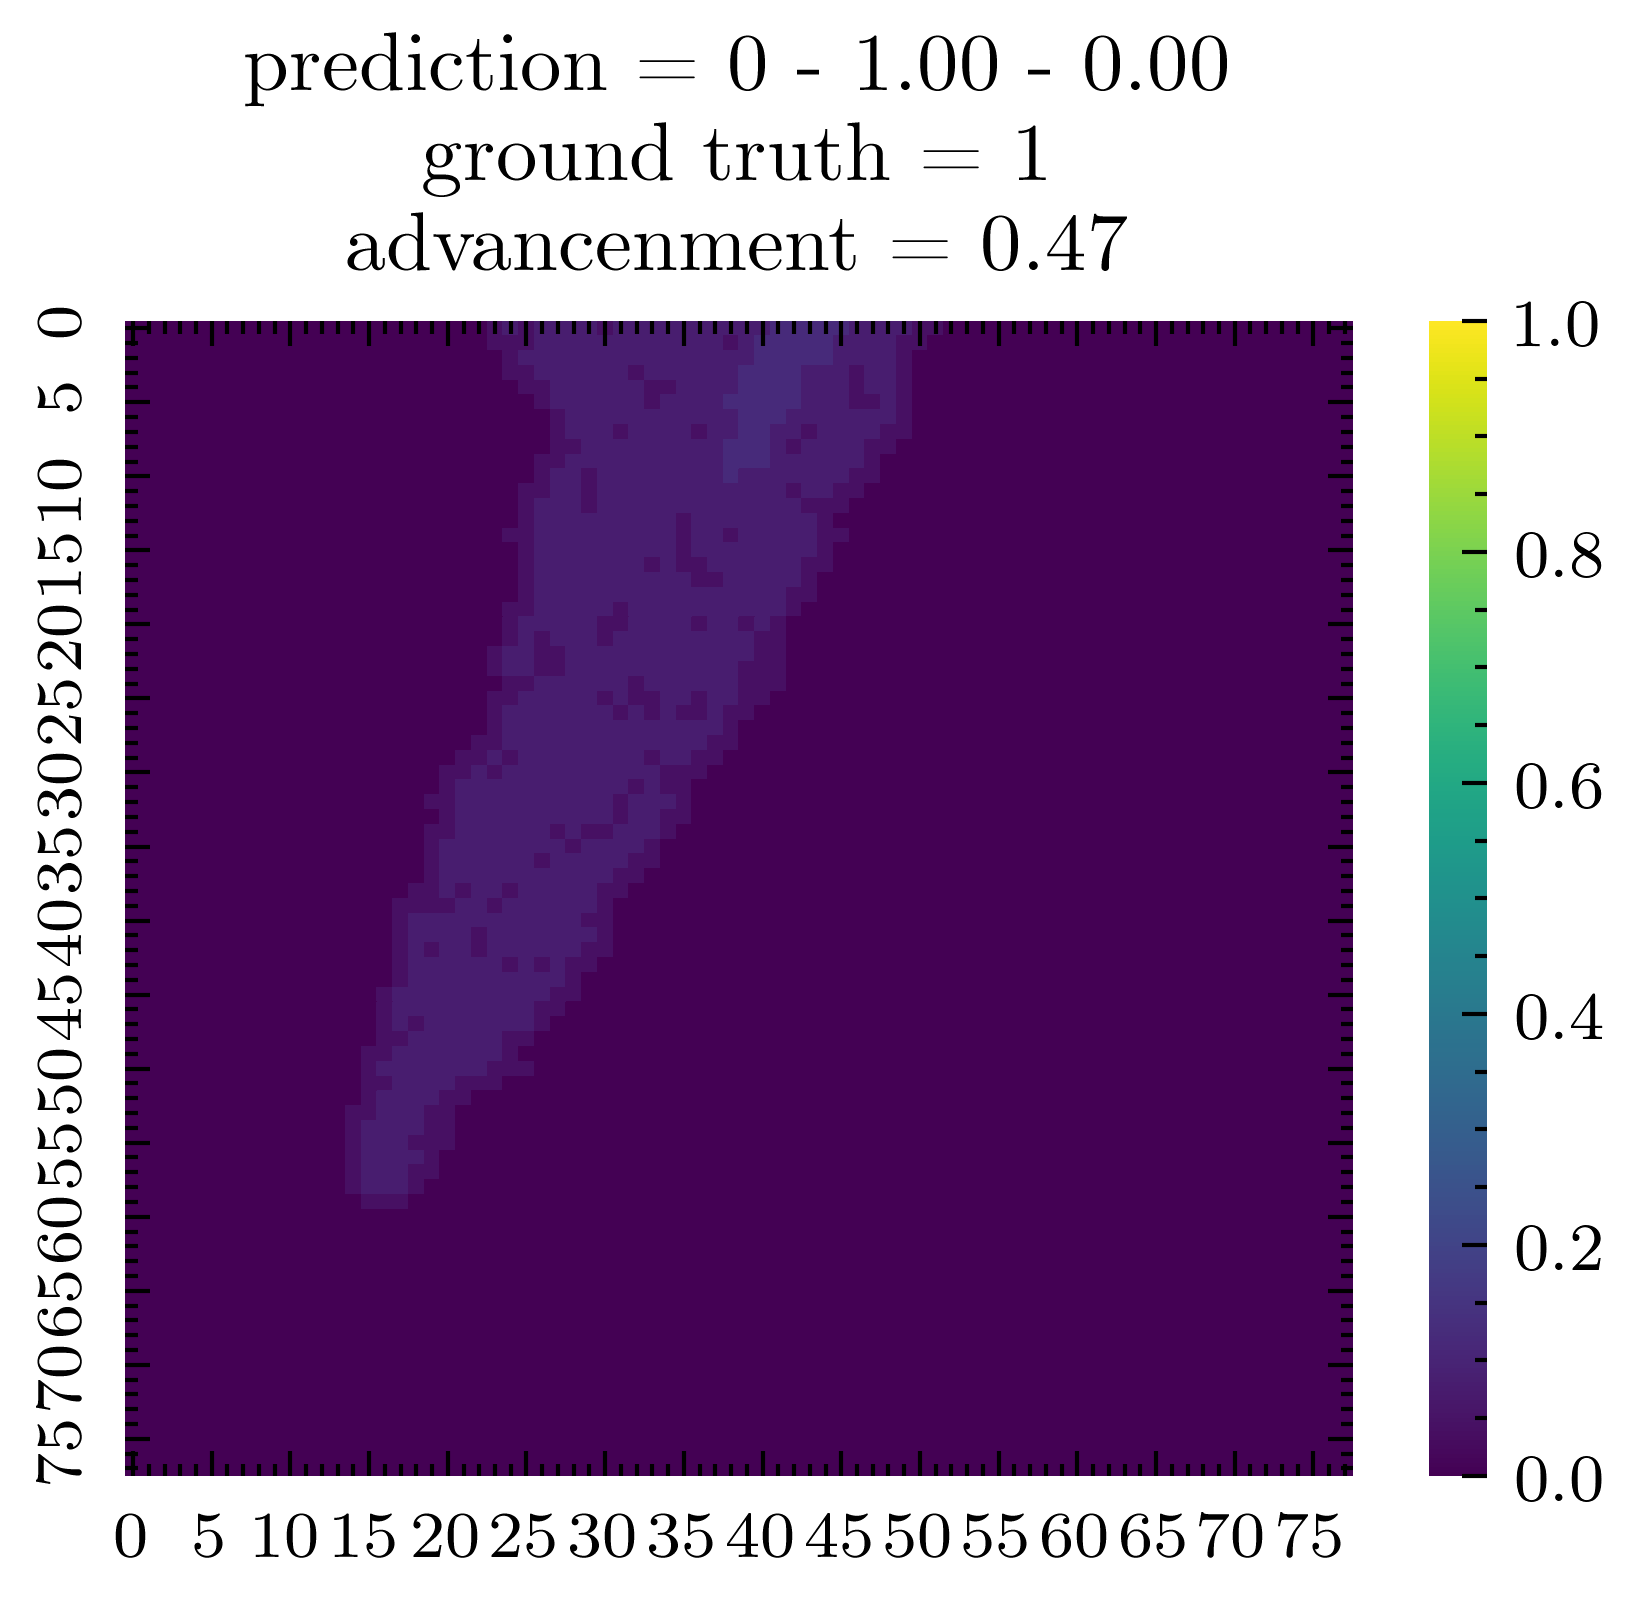
\includegraphics[width=\linewidth]{../img/5/quarry/false_positive/patch-2d-0.png}
    \end{subfigure}
    \begin{subfigure}[b]{0.19\textwidth}
        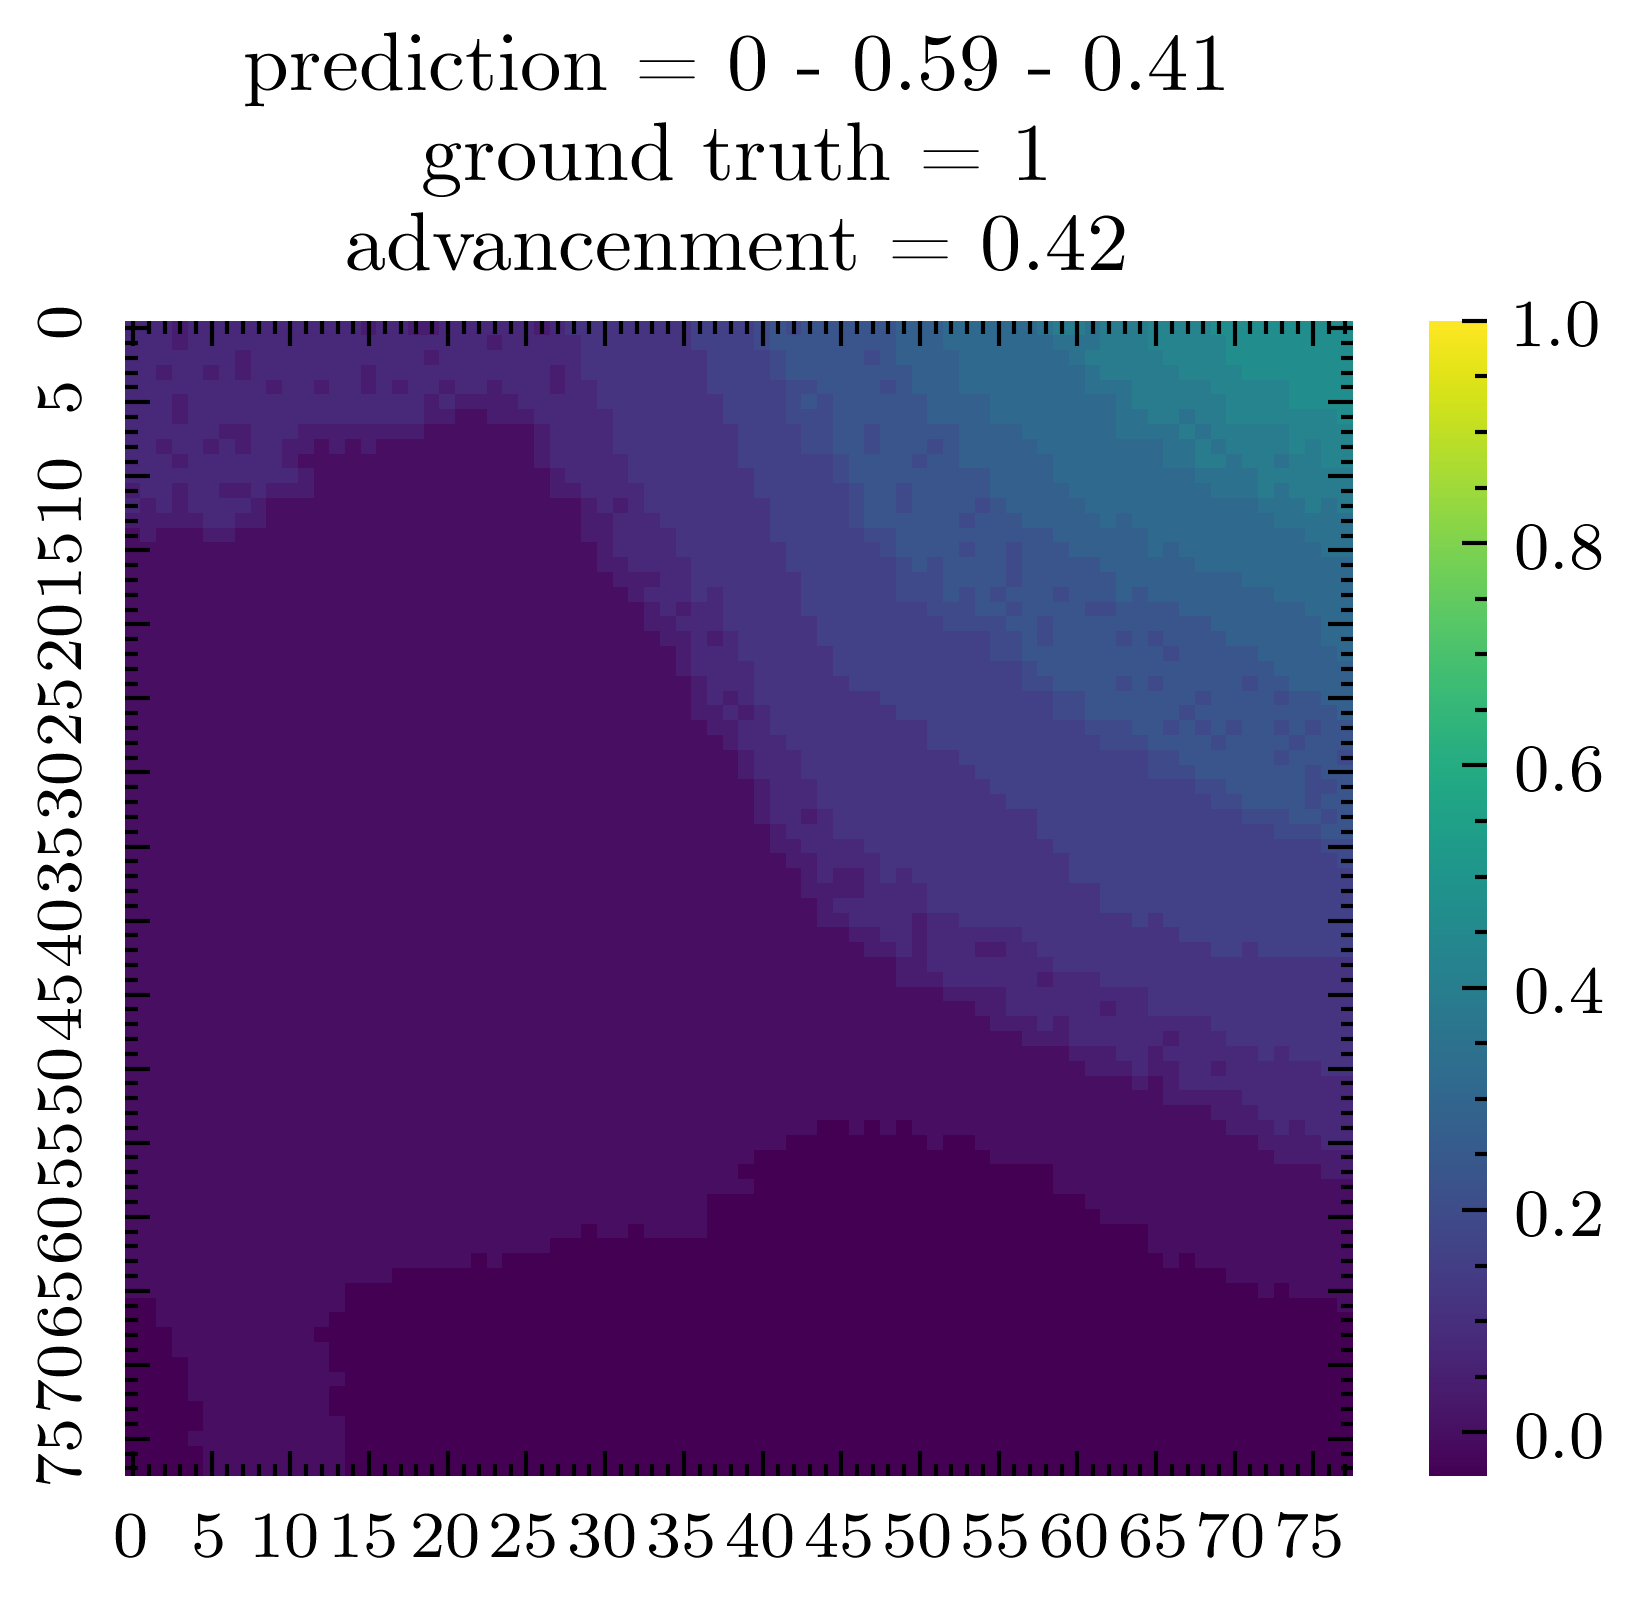
\includegraphics[width=\linewidth]{../img/5/quarry/false_positive/patch-2d-1.png}
    \end{subfigure}  
    \begin{subfigure}[b]{0.19\textwidth}
        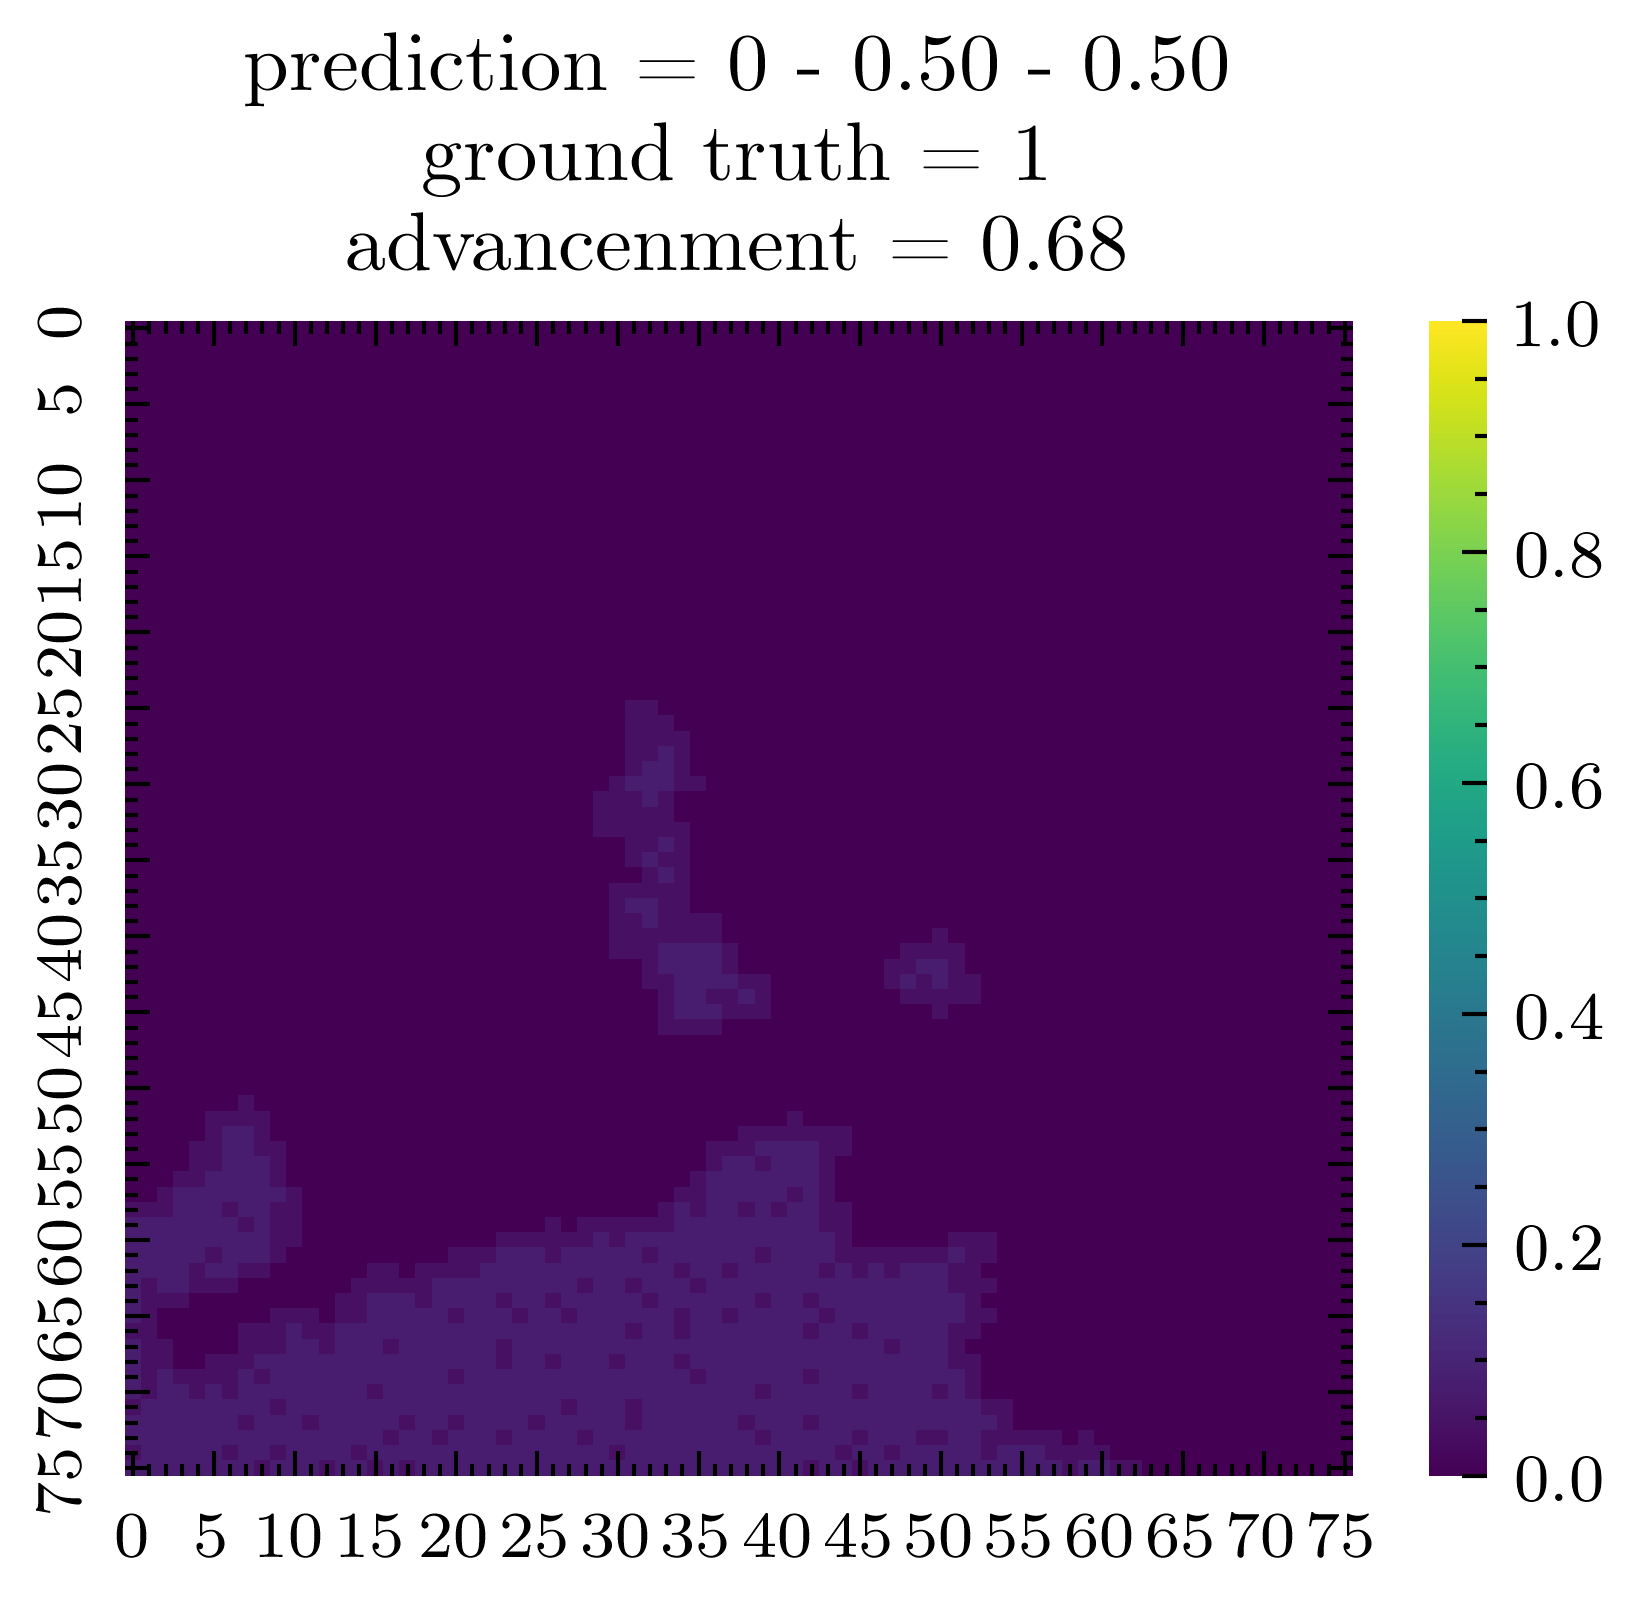
\includegraphics[width=\linewidth]{../img/5/quarry/false_positive/patch-2d-2.png}
    \end{subfigure}
    \begin{subfigure}[b]{0.19\textwidth}
        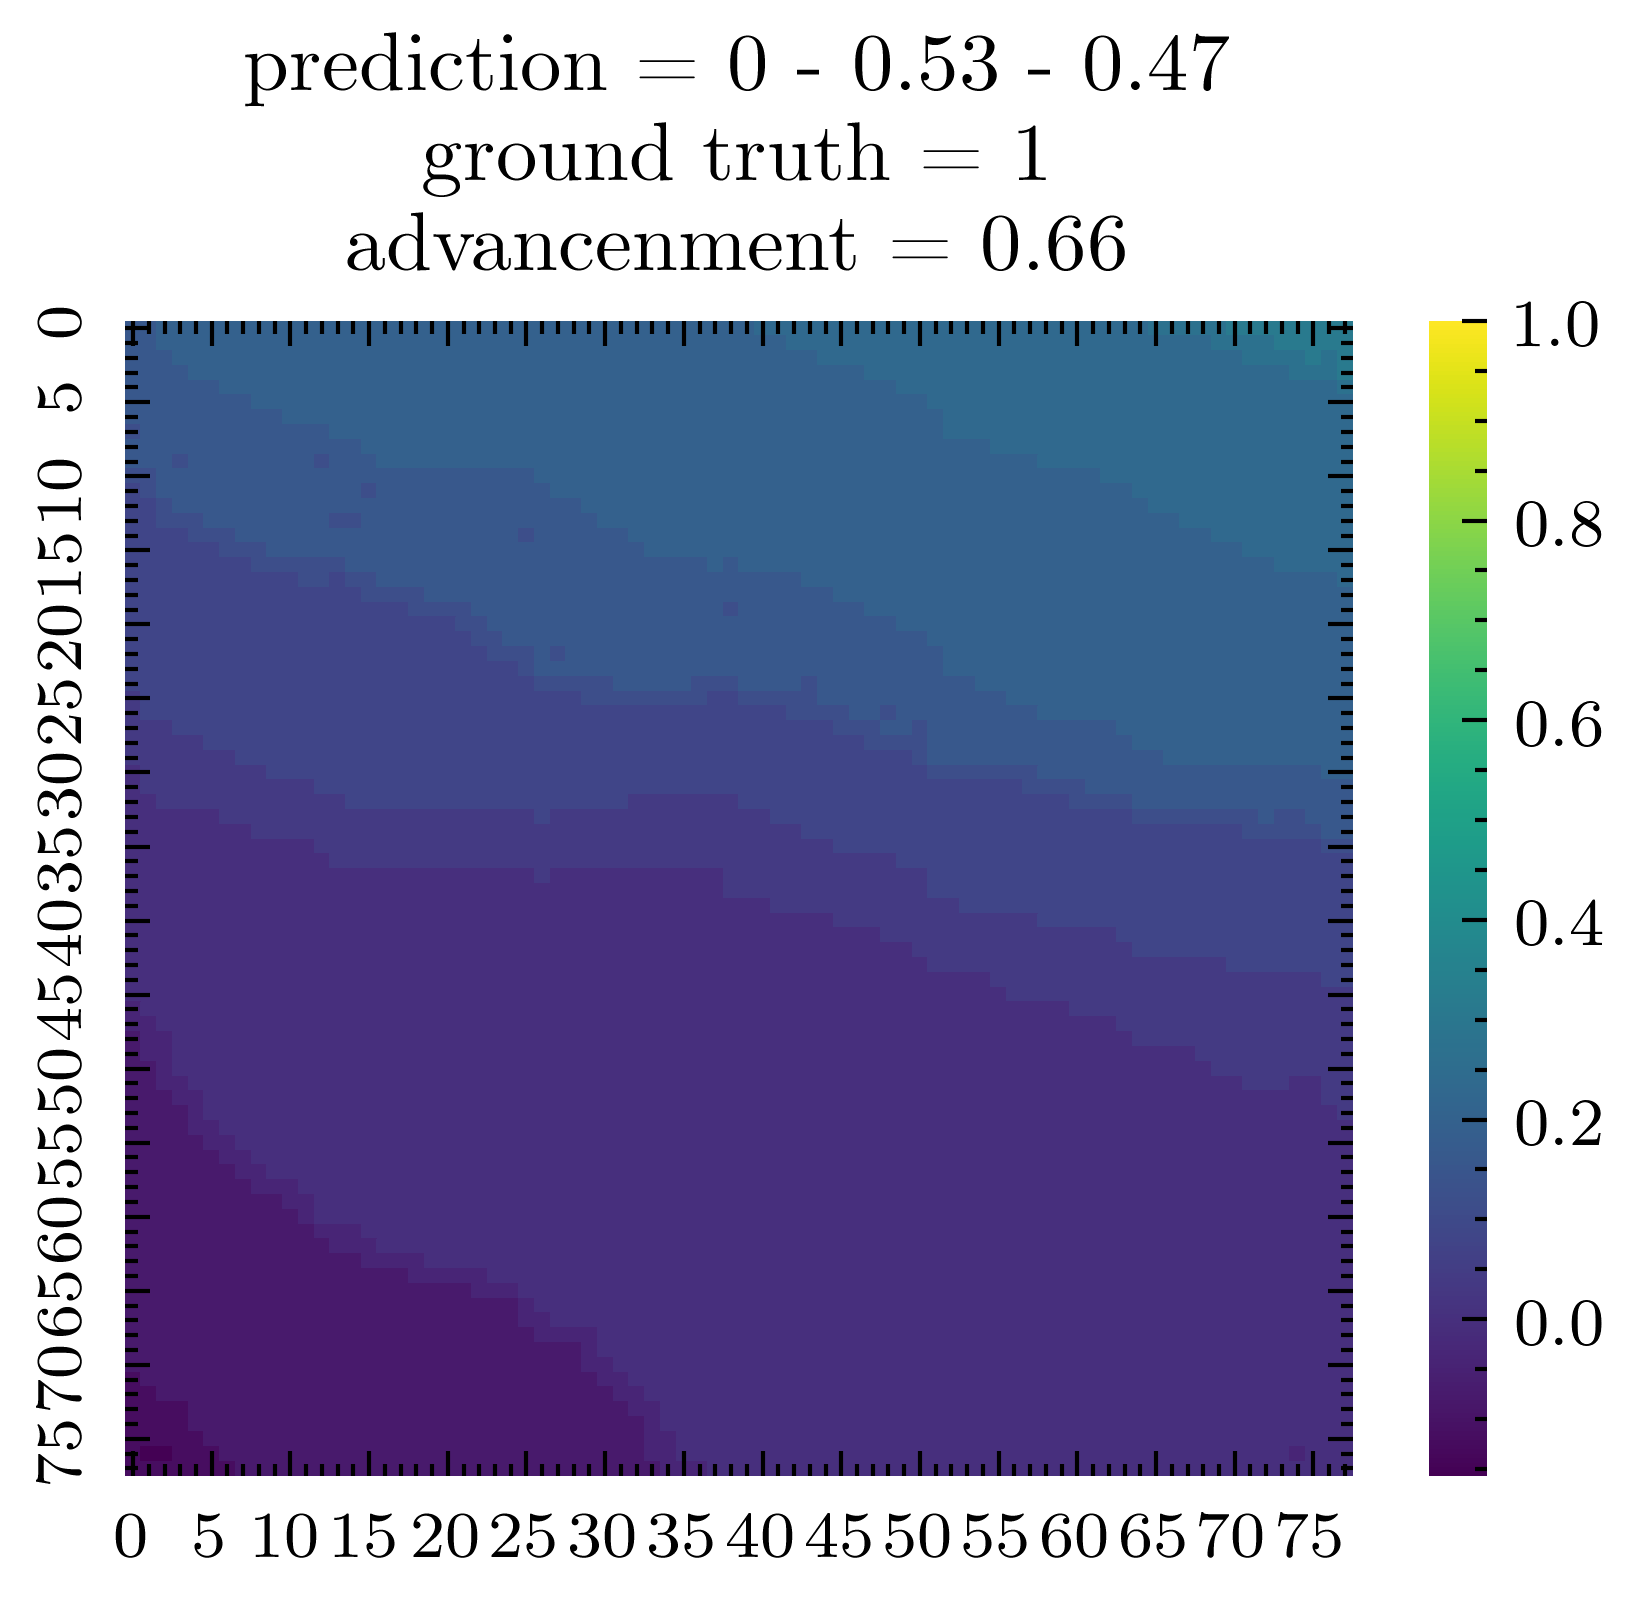
\includegraphics[width=\linewidth]{../img/5/quarry/false_positive/patch-2d-3.png}
    \end{subfigure}  
    \begin{subfigure}[b]{0.19\textwidth}
        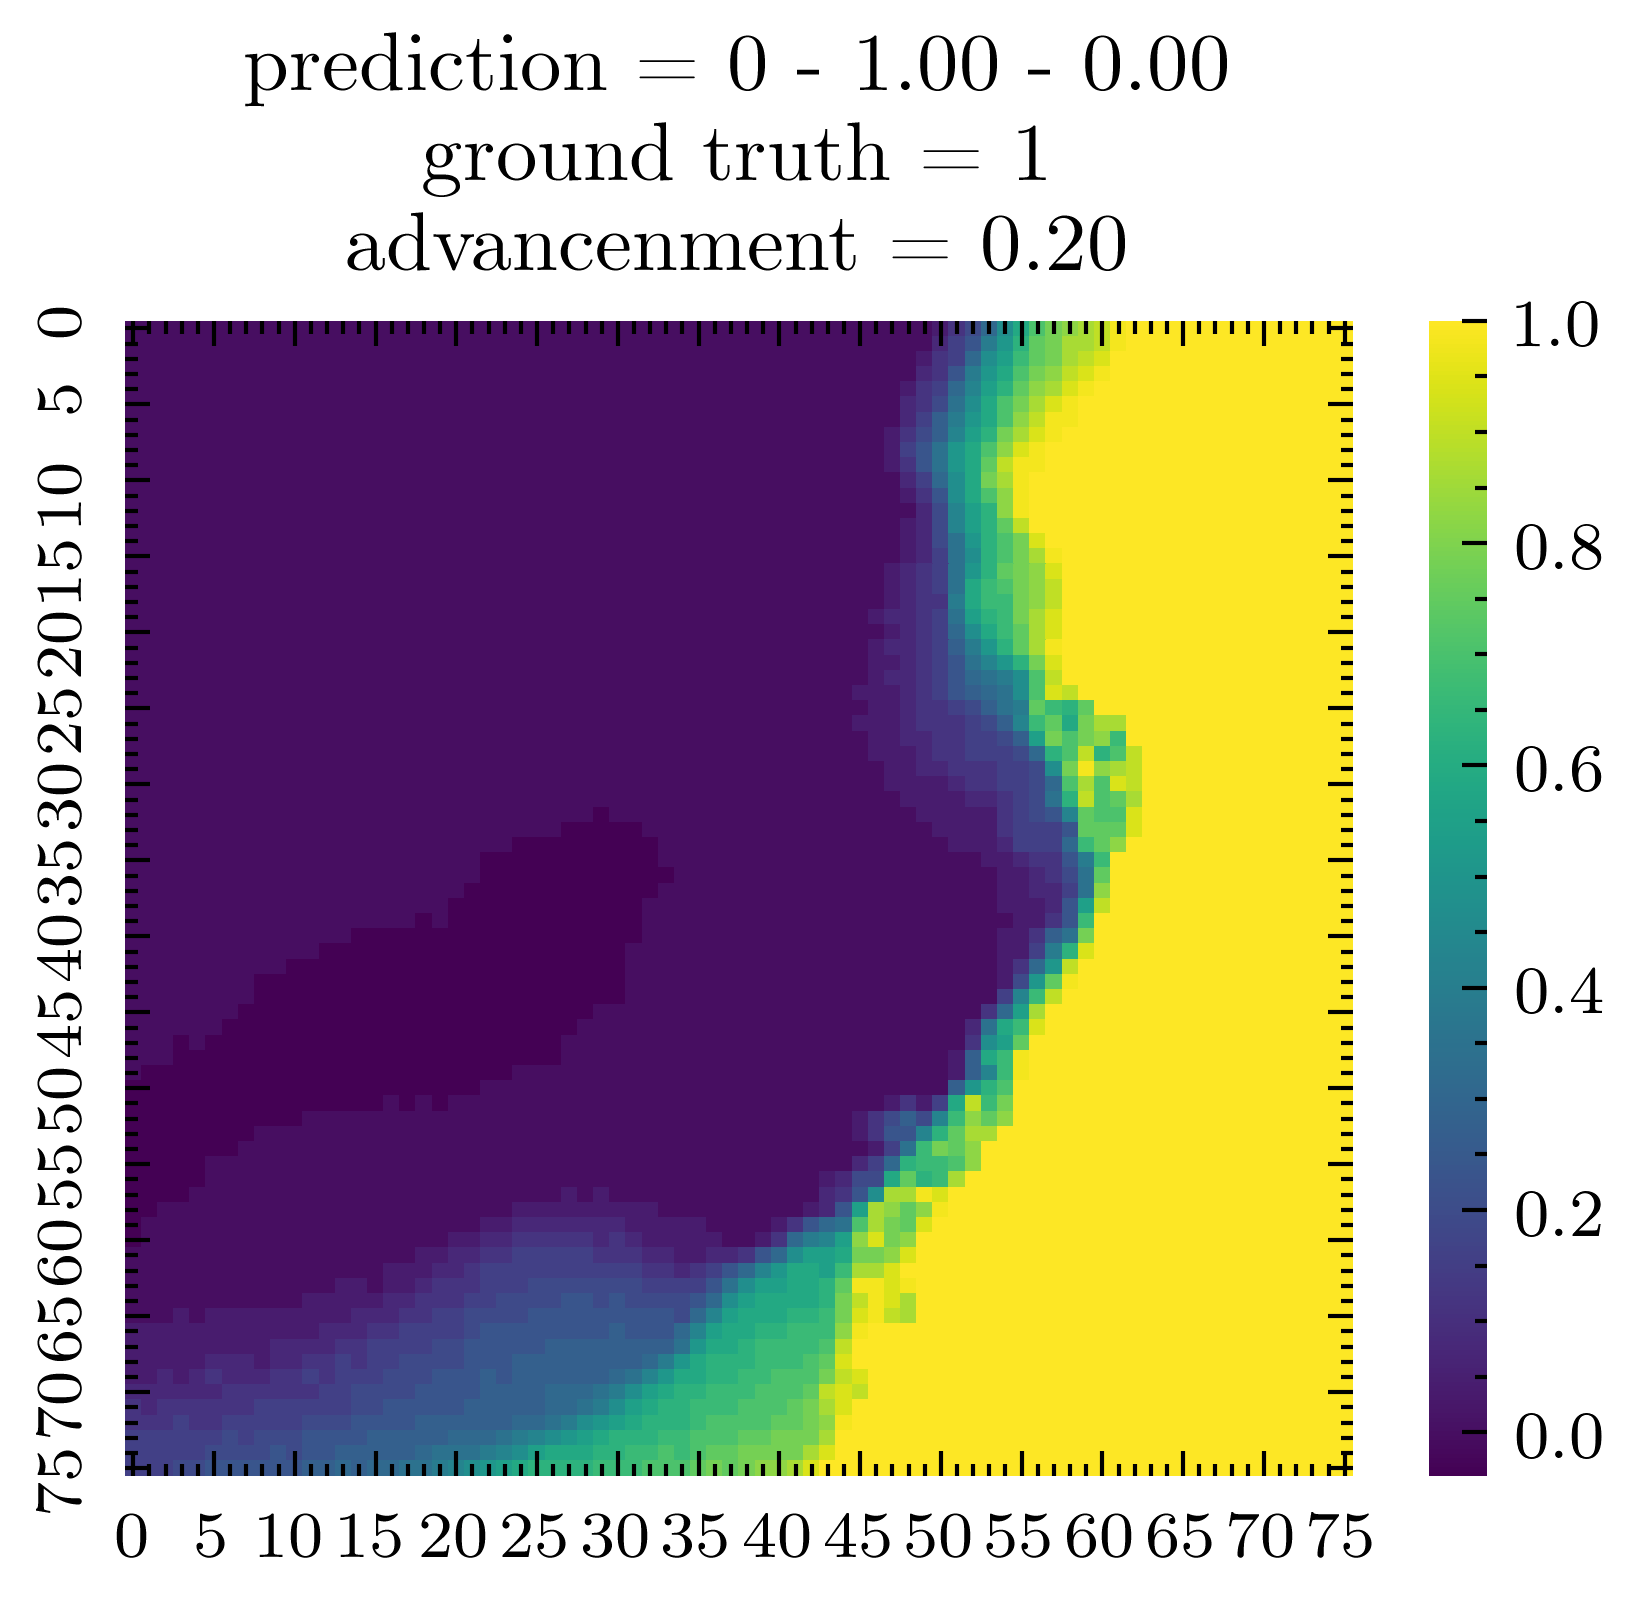
\includegraphics[width=\linewidth]{../img/5/quarry/false_positive/patch-2d-4.png}
    \end{subfigure}  

    \begin{subfigure}[b]{0.19\textwidth}
        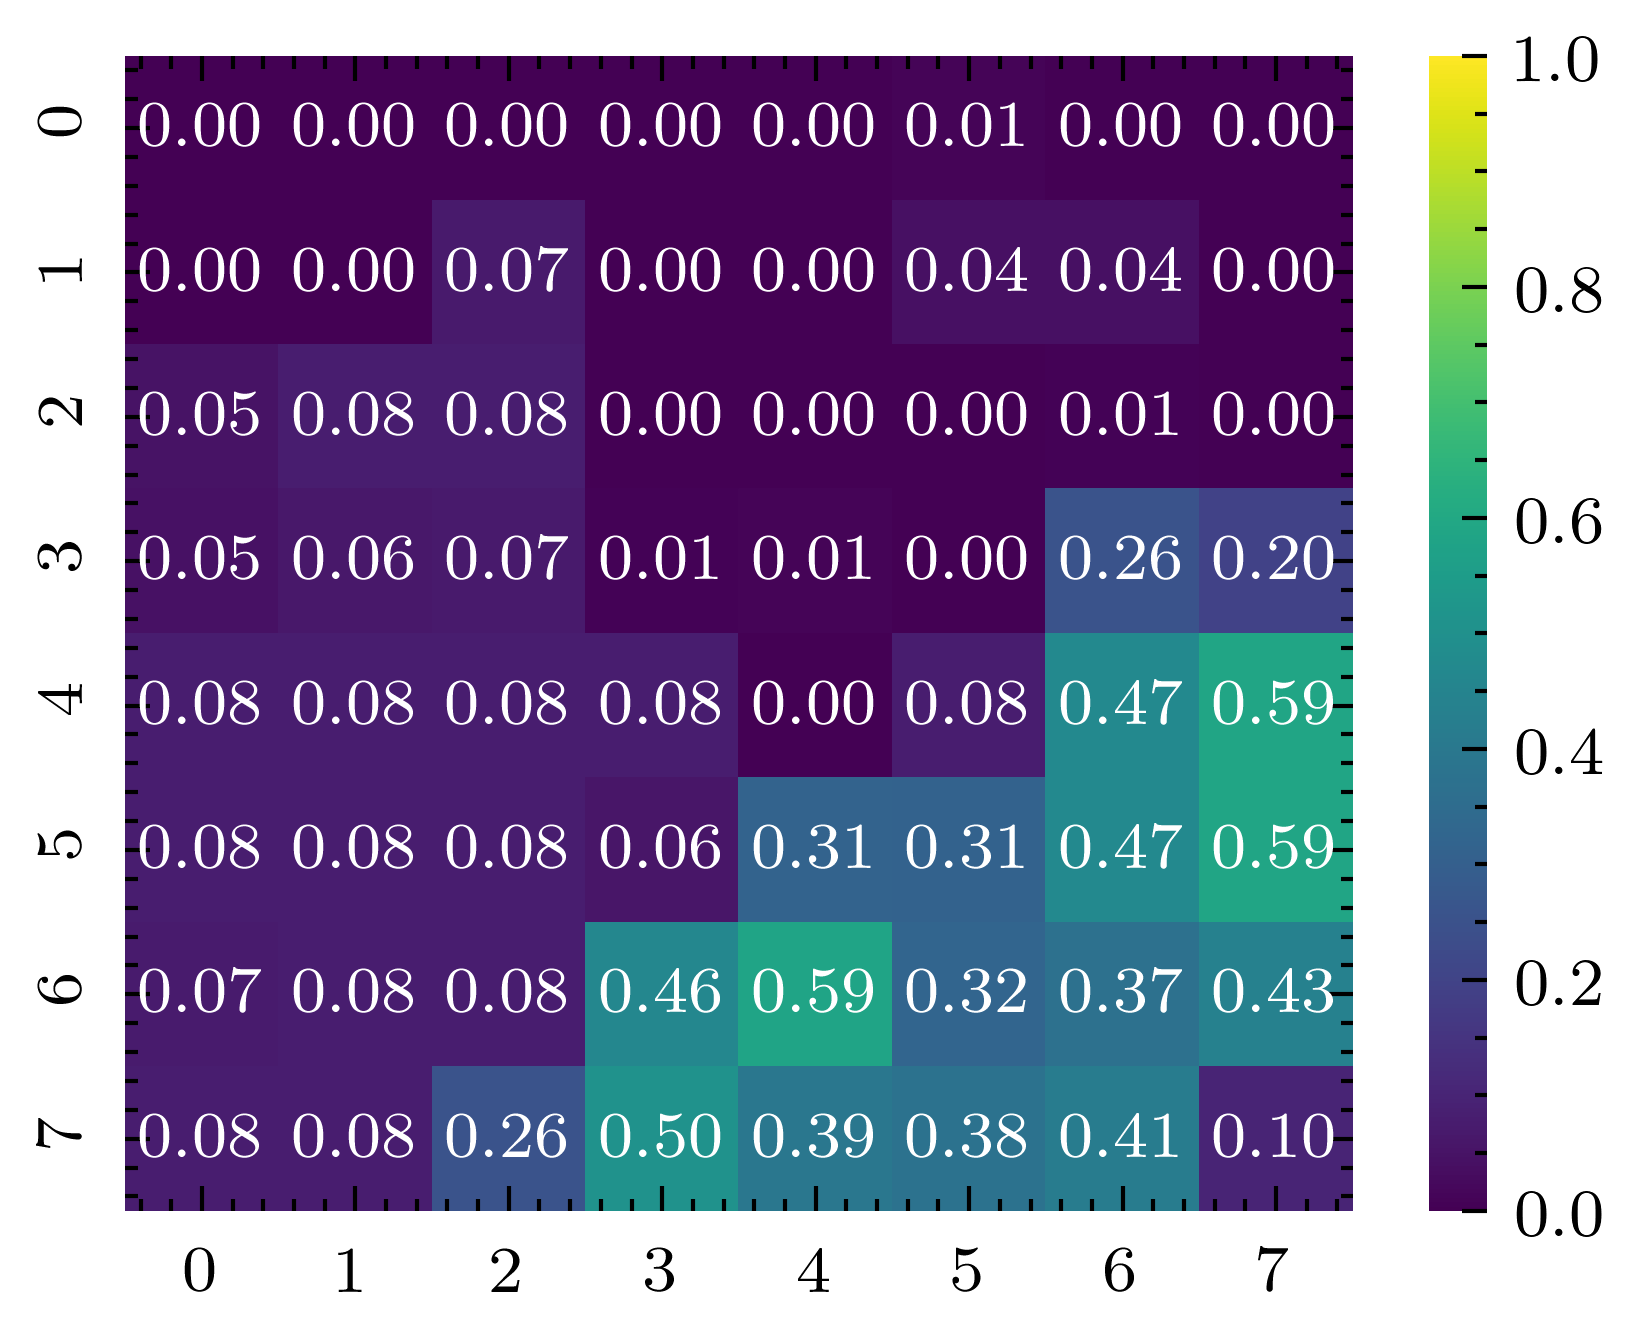
\includegraphics[width=\linewidth]{../img/5/quarry/false_positive/heatmap-2d-0.png}
    \end{subfigure}
    \begin{subfigure}[b]{0.19\textwidth}
        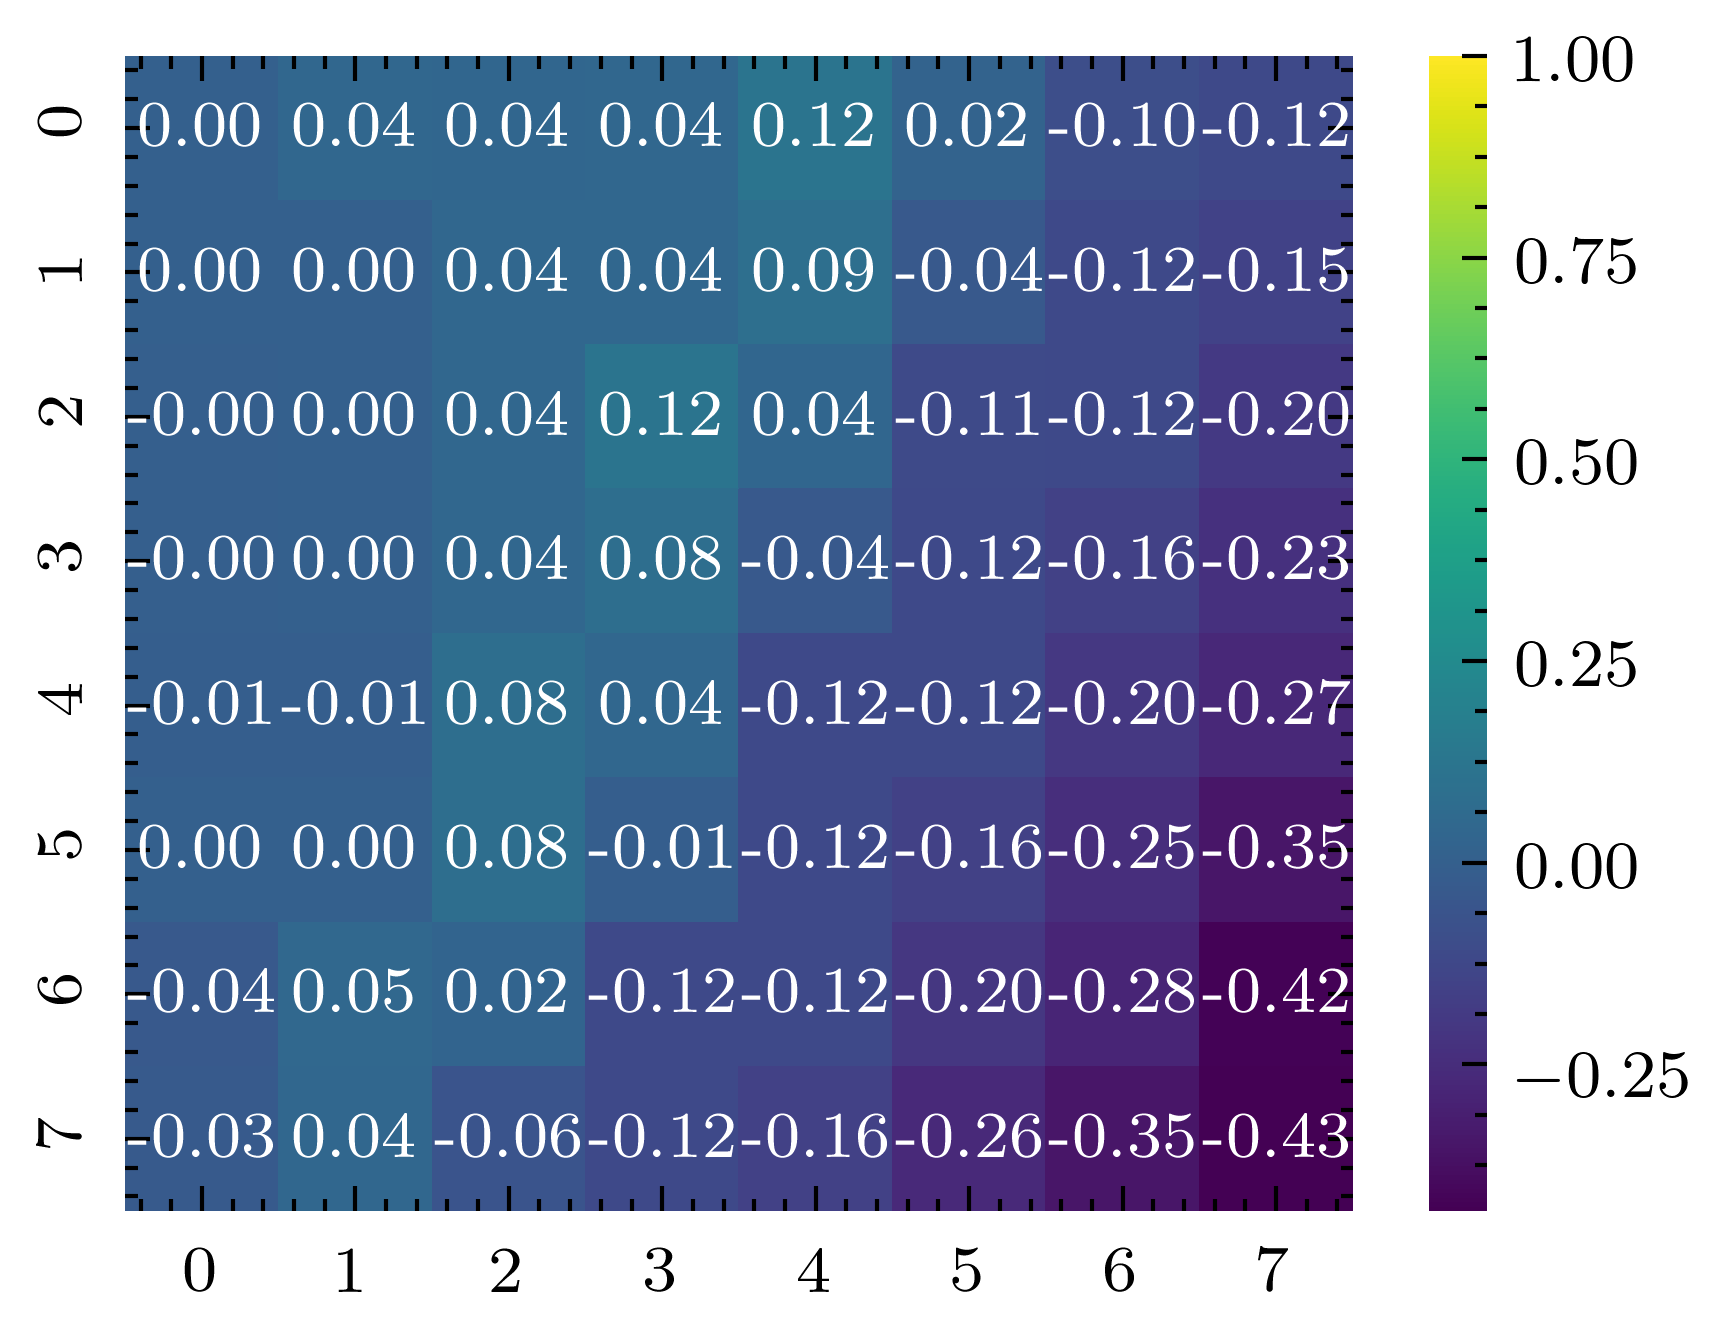
\includegraphics[width=\linewidth]{../img/5/quarry/false_positive/heatmap-2d-1.png}
    \end{subfigure}  
    \begin{subfigure}[b]{0.19\textwidth}
        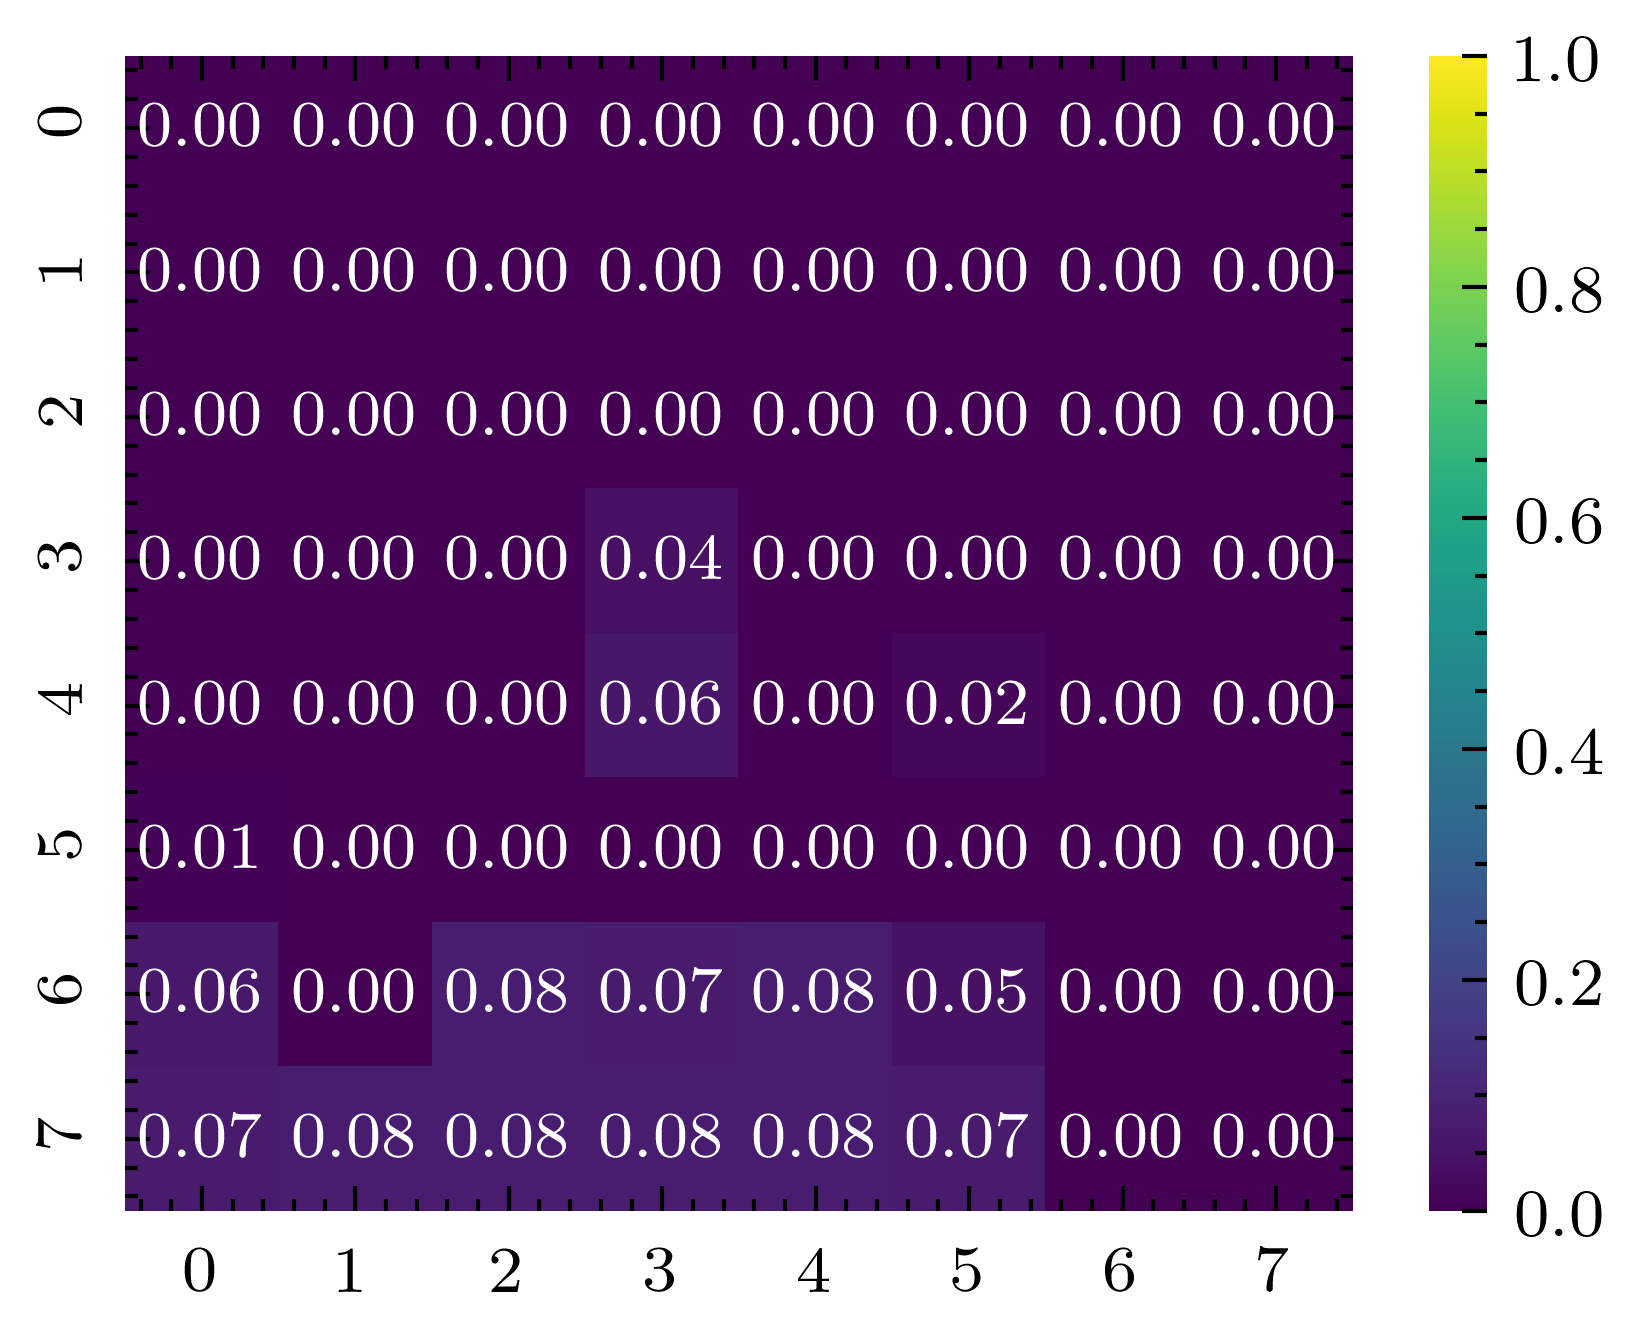
\includegraphics[width=\linewidth]{../img/5/quarry/false_positive/heatmap-2d-2.png}
    \end{subfigure}
    \begin{subfigure}[b]{0.19\textwidth}
        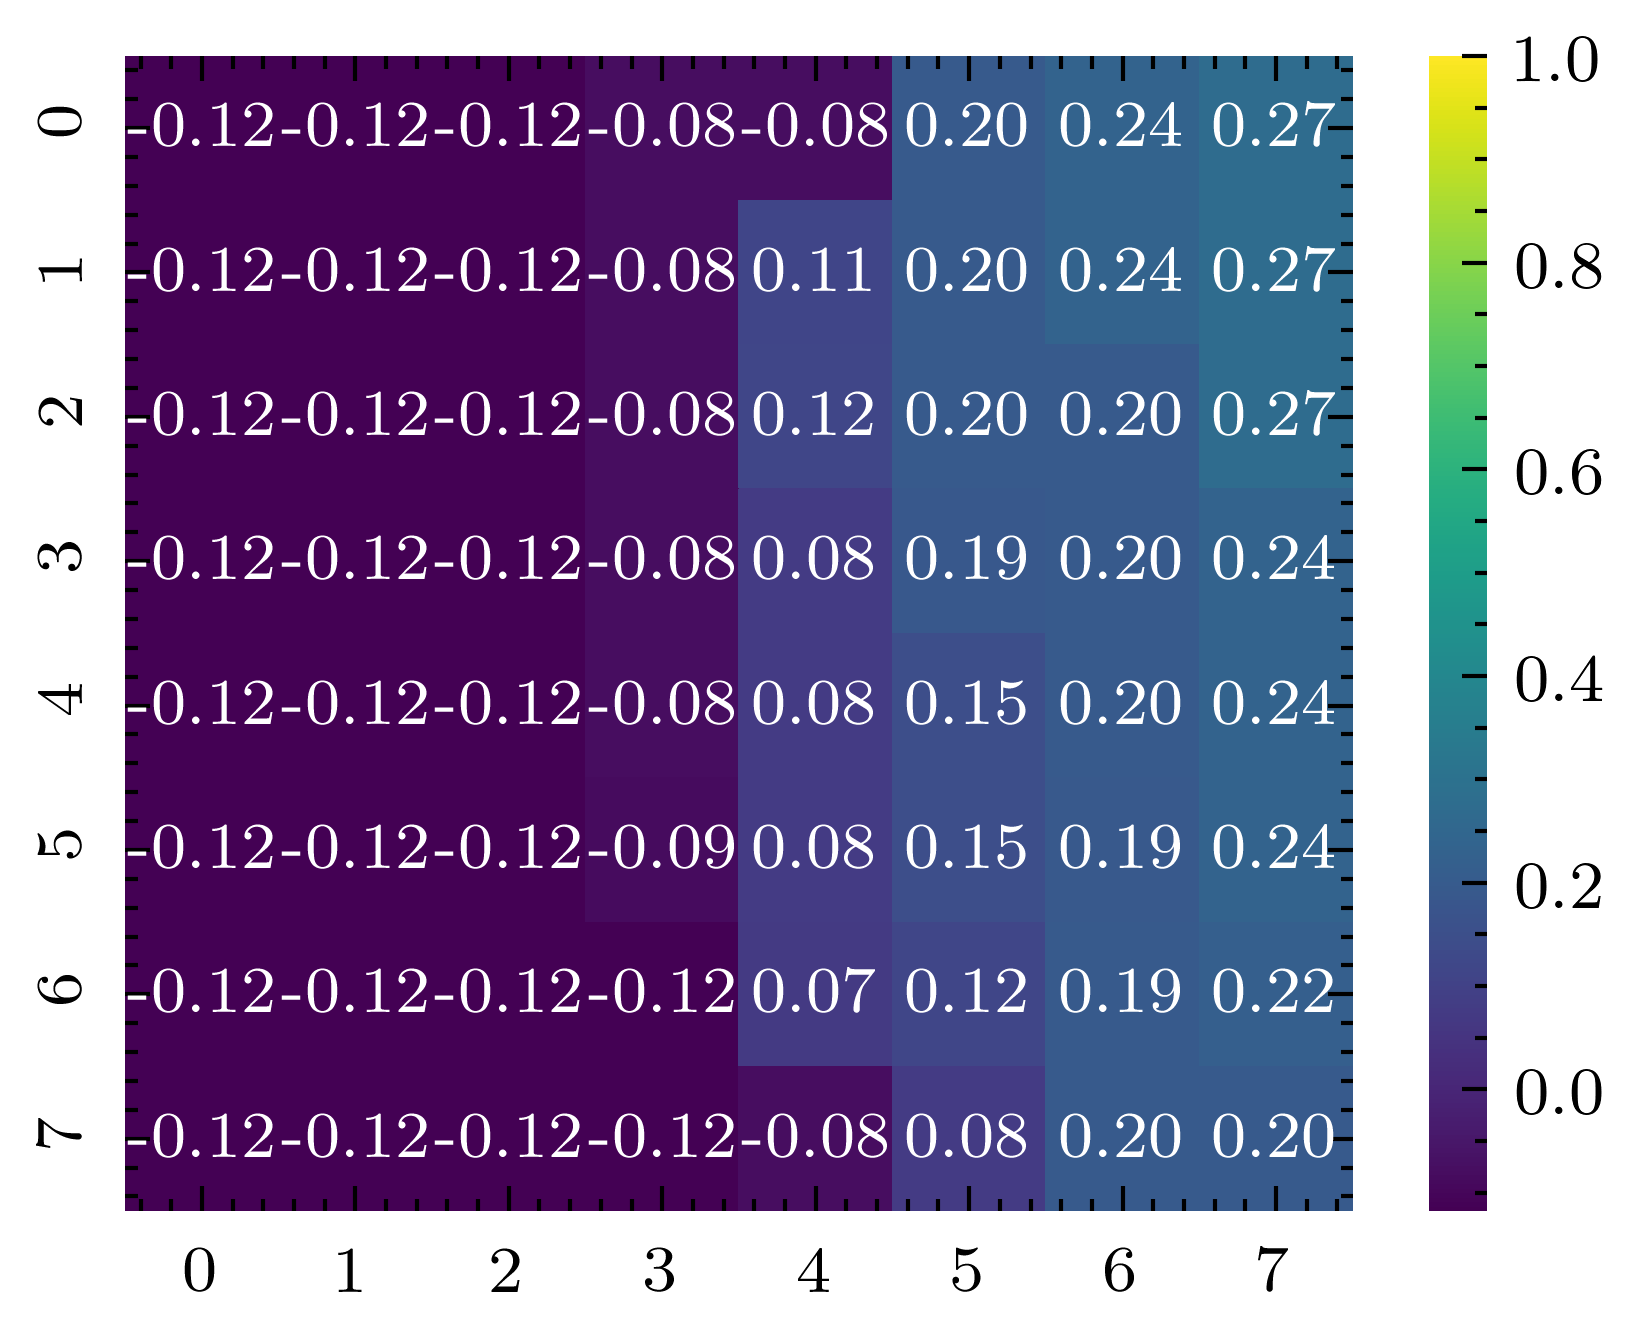
\includegraphics[width=\linewidth]{../img/5/quarry/false_positive/heatmap-2d-3.png}
    \end{subfigure}  
    \begin{subfigure}[b]{0.19\textwidth}
        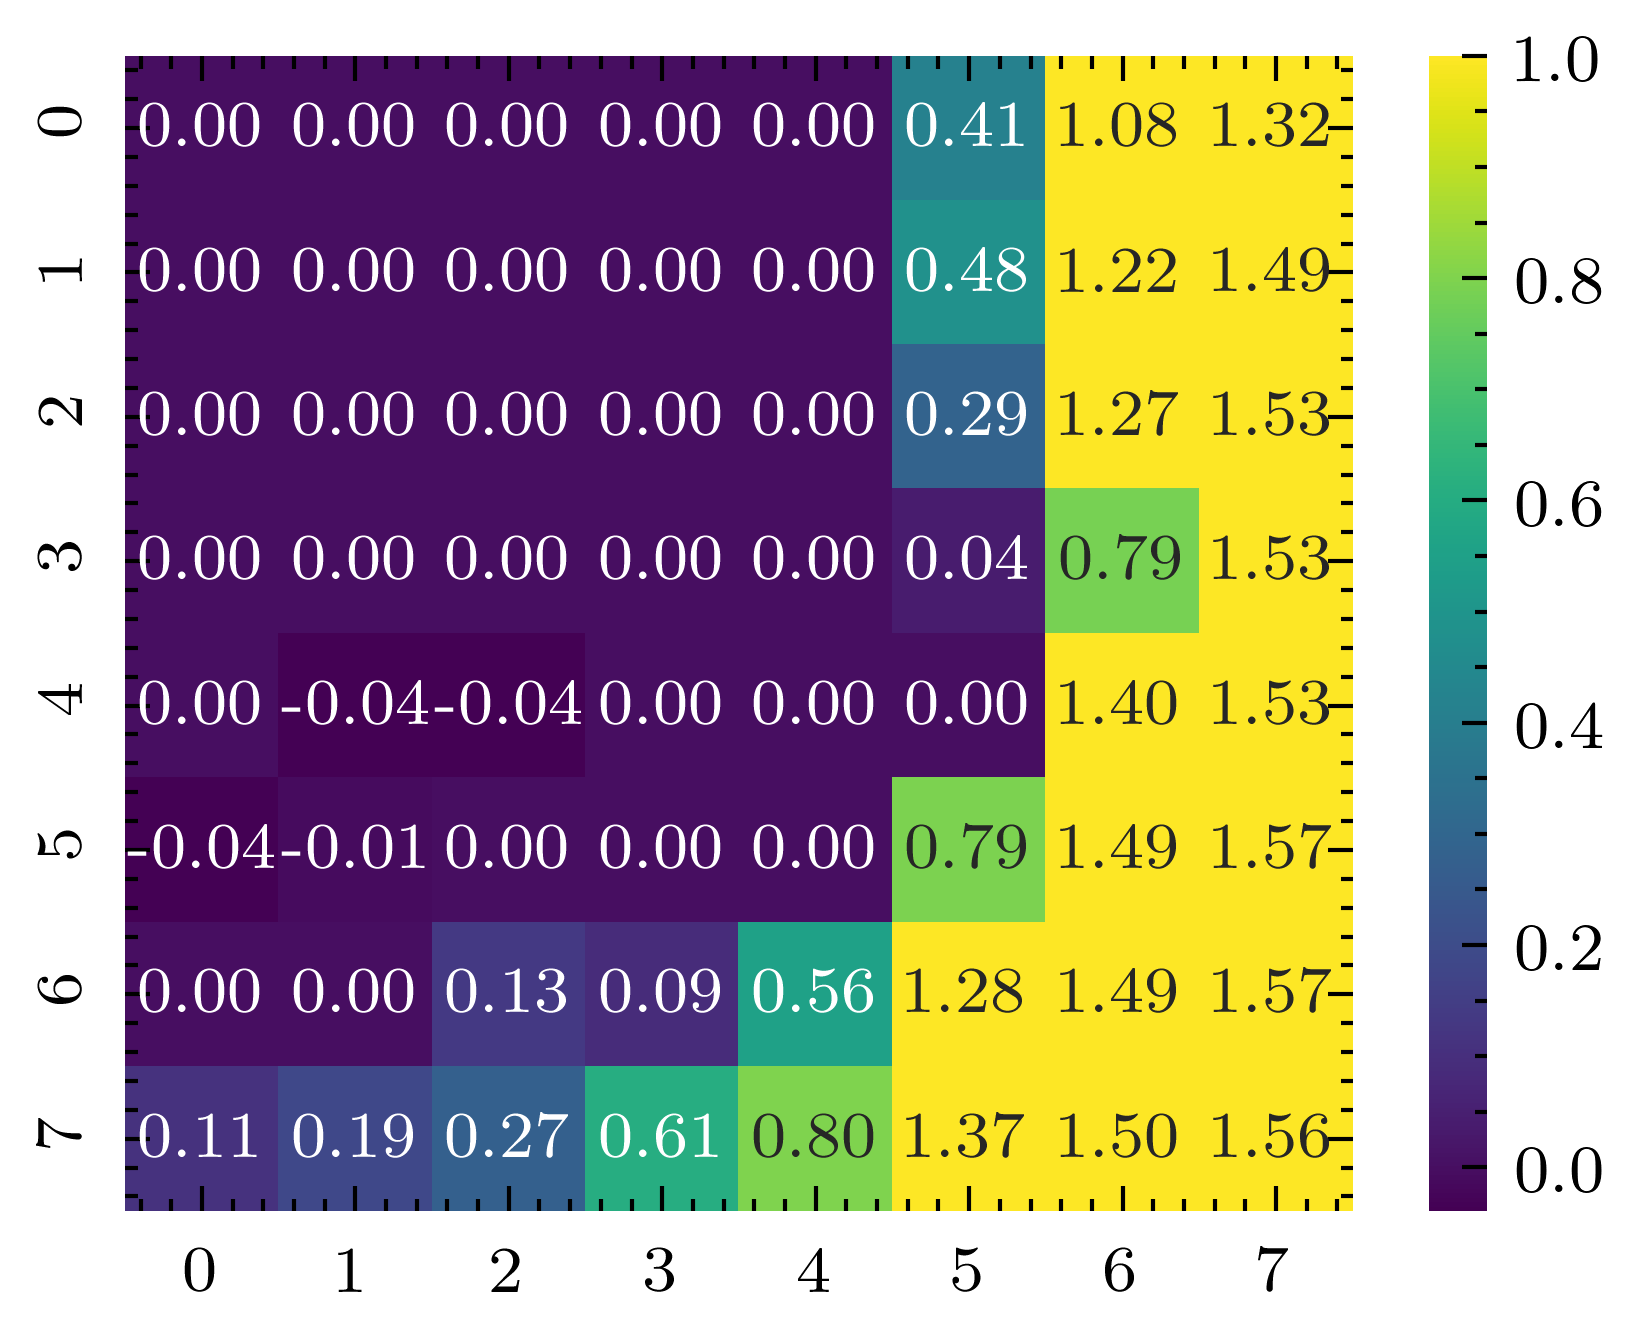
\includegraphics[width=\linewidth]{../img/5/quarry/false_positive/heatmap-2d-4.png}
    \end{subfigure}  

    \begin{subfigure}[b]{0.19\textwidth}
        \includegraphics[width=\linewidth]{../img/5/quarry/false_positive/grad-cam-2d-0.png}
    \end{subfigure}
    \begin{subfigure}[b]{0.19\textwidth}
        \includegraphics[width=\linewidth]{../img/5/quarry/false_positive/grad-cam-2d-1.png}
    \end{subfigure}  
    \begin{subfigure}[b]{0.19\textwidth}
        \includegraphics[width=\linewidth]{../img/5/quarry/false_positive/grad-cam-2d-2.png}
    \end{subfigure}
    \begin{subfigure}[b]{0.19\textwidth}
        \includegraphics[width=\linewidth]{../img/5/quarry/false_positive/grad-cam-2d-3.png}
    \end{subfigure}  
    \begin{subfigure}[b]{0.19\textwidth}
        \includegraphics[width=\linewidth]{../img/5/quarry/false_positive/grad-cam-2d-4.png}
    \end{subfigure}  

    \begin{subfigure}[b]{0.19\textwidth}
        \includegraphics[width=\linewidth]{../img/5/quarry/false_positive//patch-3d-majavi-colormap-0.png}
    \end{subfigure}
    \begin{subfigure}[b]{0.19\textwidth}
        \includegraphics[width=\linewidth]{../img/5/quarry/false_positive//patch-3d-majavi-colormap-1.png}
    \end{subfigure}  
    \begin{subfigure}[b]{0.19\textwidth}
        \includegraphics[width=\linewidth]{../img/5/quarry/false_positive//patch-3d-majavi-colormap-2.png}
    \end{subfigure}
    \begin{subfigure}[b]{0.19\textwidth}
        \includegraphics[width=\linewidth]{../img/5/quarry/false_positive//patch-3d-majavi-colormap-3.png}
    \end{subfigure}  
    \begin{subfigure}[b]{0.19\textwidth}
        \includegraphics[width=\linewidth]{../img/5/quarry/false_positive//patch-3d-majavi-colormap-4.png}
    \end{subfigure}  

\caption{False Positive}    
\end{figure}


\begin{figure}[H]
    \centering
    \begin{subfigure}[b]{0.19\textwidth}
        \includegraphics[width=\linewidth]{../img/5/quarry/false_negative/patch-2d-0.png}
    \end{subfigure}
    \begin{subfigure}[b]{0.19\textwidth}
        \includegraphics[width=\linewidth]{../img/5/quarry/false_negative/patch-2d-1.png}
    \end{subfigure}  
    \begin{subfigure}[b]{0.19\textwidth}
        \includegraphics[width=\linewidth]{../img/5/quarry/false_negative/patch-2d-2.png}
    \end{subfigure}
    \begin{subfigure}[b]{0.19\textwidth}
        \includegraphics[width=\linewidth]{../img/5/quarry/false_negative/patch-2d-3.png}
    \end{subfigure}  
    \begin{subfigure}[b]{0.19\textwidth}
        \includegraphics[width=\linewidth]{../img/5/quarry/false_negative/patch-2d-4.png}
    \end{subfigure}  

    \begin{subfigure}[b]{0.19\textwidth}
        \includegraphics[width=\linewidth]{../img/5/quarry/false_negative/heatmap-2d-0.png}
    \end{subfigure}
    \begin{subfigure}[b]{0.19\textwidth}
        \includegraphics[width=\linewidth]{../img/5/quarry/false_negative/heatmap-2d-1.png}
    \end{subfigure}  
    \begin{subfigure}[b]{0.19\textwidth}
        \includegraphics[width=\linewidth]{../img/5/quarry/false_negative/heatmap-2d-2.png}
    \end{subfigure}
    \begin{subfigure}[b]{0.19\textwidth}
        \includegraphics[width=\linewidth]{../img/5/quarry/false_negative/heatmap-2d-3.png}
    \end{subfigure}  
    \begin{subfigure}[b]{0.19\textwidth}
        \includegraphics[width=\linewidth]{../img/5/quarry/false_negative/heatmap-2d-4.png}
    \end{subfigure}  

    \begin{subfigure}[b]{0.19\textwidth}
        \includegraphics[width=\linewidth]{../img/5/quarry/false_negative/grad-cam-2d-0.png}
    \end{subfigure}
    \begin{subfigure}[b]{0.19\textwidth}
        \includegraphics[width=\linewidth]{../img/5/quarry/false_negative/grad-cam-2d-1.png}
    \end{subfigure}  
    \begin{subfigure}[b]{0.19\textwidth}
        \includegraphics[width=\linewidth]{../img/5/quarry/false_negative/grad-cam-2d-2.png}
    \end{subfigure}
    \begin{subfigure}[b]{0.19\textwidth}
        \includegraphics[width=\linewidth]{../img/5/quarry/false_negative/grad-cam-2d-3.png}
    \end{subfigure}  
    \begin{subfigure}[b]{0.19\textwidth}
        \includegraphics[width=\linewidth]{../img/5/quarry/false_negative/grad-cam-2d-4.png}
    \end{subfigure}  

    \begin{subfigure}[b]{0.19\textwidth}
        \includegraphics[width=\linewidth]{../img/5/quarry/false_negative//patch-3d-majavi-colormap-0.png}
    \end{subfigure}
    \begin{subfigure}[b]{0.19\textwidth}
        \includegraphics[width=\linewidth]{../img/5/quarry/false_negative//patch-3d-majavi-colormap-1.png}
    \end{subfigure}  
    \begin{subfigure}[b]{0.19\textwidth}
        \includegraphics[width=\linewidth]{../img/5/quarry/false_negative//patch-3d-majavi-colormap-2.png}
    \end{subfigure}
    \begin{subfigure}[b]{0.19\textwidth}
        \includegraphics[width=\linewidth]{../img/5/quarry/false_negative//patch-3d-majavi-colormap-3.png}
    \end{subfigure}  
    \begin{subfigure}[b]{0.19\textwidth}
        \includegraphics[width=\linewidth]{../img/5/quarry/false_negative//patch-3d-majavi-colormap-4.png}
    \end{subfigure}  

\caption{False Negative}    
\end{figure}

\subsection{Robustness}
In this section we test the model against custom patches with different features. For most of those patches, we know what to expect.

\subsubsection{Walls}
We can start by exploring models behaviour against different walls at different positions. The easiest test we can do is placing a non traversable wall various position in front of \emph{Krock}

\end{document}